%%
%% ACS project dissertation template.
%%
%% Currently designed for printing two-sided, but if you prefer to
%% print single-sided just remove ",twoside,openright" from the
%% \documentclass[] line below.
%%
%%
%%   SMH, May 2010.


\documentclass[a4paper,12pt]{report}


%%
%% EDIT THE BELOW TO CUSTOMIZE
%%

\def\authorname{Yiren (Aaron) Zhao\xspace}
\def\authorcollege{Corpus Christi College\xspace}
\def\authoremail{yaz21@cam.ac.uk}
\def\dissertationtitle{Improving Compression Pipelines For Convolutional Neural Networks}
\def\wordcount{14,235}


\usepackage{epsfig,graphicx,parskip,setspace,tabularx,xspace,amsmath}
\usepackage{cleveref}
\usepackage{pgf}
\usepackage{tikz}
\usepackage[utf8]{inputenc}
\usepackage{algorithm}
\usepackage{algorithmic}
% \usepackage[noend]{algpseudocode}

\usetikzlibrary{arrows,automata}
\usetikzlibrary{positioning}
\tikzstyle{box} = [rectangle, fill={rgb:black,1;white,2.5}, rounded corners, minimum width=4cm, minimum height=2cm, text centered, draw=black]
\tikzstyle{myarrows}=[line width=1mm,draw=black,-triangle 45,postaction={draw, line width=3mm, shorten >=4mm, -}]


\begin{document}


%% FRONTMATTER (TITLE PAGE, DECLARATION, ABSTRACT, ETC)
\pagestyle{empty}
\singlespacing
% title page information
\begin{titlepage} 

\begin{center}
\noindent
\huge
\dissertationtitle \\
\vspace*{\stretch{1}}
\end{center}

\begin{center}
\noindent
\huge
\authorname \\
\Large
\authorcollege      \\[24pt]

\includegraphics{CUni3.eps}
\end{center}

\vspace{24pt} 

\begin{center}
\noindent
\large
{\it A dissertation submitted to the University of Cambridge \\ 
in partial fulfilment of the requirements for the degree of \\ 
Master of Philosophy in Advanced Computer Science} 
\vspace*{\stretch{1}}
\end{center}

\begin{center}
\noindent
University of Cambridge \\
Computer Laboratory     \\
William Gates Building  \\
15 JJ Thomson Avenue    \\
Cambridge CB3 0FD       \\
{\sc United Kingdom}    \\
\end{center}

\begin{center}
\noindent
Email: \authoremail \\
\end{center}

\begin{center}
\noindent
\today
\end{center}

\end{titlepage} 

\newpage
\vspace*{\fill}

\onehalfspacing
\newpage
{\Huge \bf Declaration}

\vspace{24pt} 

I \authorname of \authorcollege, being a candidate for the M.Phil in
Advanced Computer Science, hereby declare that this report and the
work described in it are my own work, unaided except as may be
specified below, and that the report does not contain material that
has already been used to any substantial extent for a comparable
purpose.

\vspace{24pt}
Total word count: \wordcount

\vspace{60pt}
\textbf{Signed}: 

\vspace{12pt}
\textbf{Date}:


\vfill

This dissertation is copyright \copyright 2010 \authorname. 
\\
All trademarks used in this dissertation are hereby acknowledged.



\newpage
\vspace*{\fill}

\singlespacing
\newpage
{\Huge \bf Abstract}
\vspace{24pt} 


This is the abstract. Write a summary of the whole thing. Make 
sure it fits in one page. 


\newpage
\vspace*{\fill}


\pagenumbering{roman}
\setcounter{page}{0}
\pagestyle{plain}
\tableofcontents
\listoffigures
\listoftables

\onehalfspacing

%% START OF MAIN TEXT

\chapter{Introduction}
\pagenumbering{arabic}
\setcounter{page}{1}

Neural Networks have achieved outstanding accuracies in large-scale
image classifications and they are becoming a state-of-art technique for
solving problems in computer vision  \cite{Krizhevsky,Lecun1998gradient,
Szegedy}.

It is the rise of deep neural network, in particular, that has helped researchers
to achieve outstanding accuracies on many popular datasets.
In 1998, \textit{Lecun et al.} proposed a 5-layer network called \textit{LeNet5}
for recognising hand-written digits \cite{Lecun1998gradient}.
\textit{Lecun et al.} utilised around 1M parameters to achieve a good accuracy on
this particular recognition task.
\textit{AlexNet}, designed by \textit{Krizhevsky et al.} for the 2012 ImageNet
competition, trained on 1.2 million images
and was used for classification with $1000$ categories \cite{Krizhevsky}.
The $1000$ classes include every-day objects (cat, dog, leopard and etc), and the proposed
\textit{AlexNet} utilized around 60 million parameters \cite{Krizhevsky}.
\textit{Coates et al.} scaled up the learning algorithm to utilise over
11 billion parameters and ran it on 16 machines to recognise unlabelled human
faces \cite{Coates}.
Neural networks are becoming deeper and are utilizing a larger number of parameters
for harder recognition problems.

\Cref{tab:networkmodels} summarized some popular networks, the results show the
trend that neural networks are going deeper.
Before 2014, researchers focus on designing large neural networks to improve
error rates on the \textit{ImageNet} dataset \cite{deng2009imagenet}.
\textit{AlexNet} and \textit{VGG16} both use stacked fully connected layers and
convolutional layers \cite{Krizhevsky, DBLP:journals/corr/SimonyanZ14a}, and
consumed a larger number of parameters.
After 2014, researchers starts to develop more efficient network
architectures and training methodologies.
\textit{InceptionV3} uses \textit{Batch normalization} \cite{DBLP:journals/corr/IoffeS15}
and factorizes traditional large convolutional kernels into small convolutional kernels \cite{DBLP:journals/corr/SzegedyVISW15}.
\textit{ResNet200} makes use of shortcut connections, these connections skip one
or multiple layers \cite{DBLP:journals/corr/HeZRS15}.
\Cref{fig:network_size} gives an overview of the networks mentioned above by considering
their top-5 error rates and sizes when used on the \textit{ILSVRC 2012} dataset \cite{deng2009imagenet}.
\textit{ResNet200} strikes the best balance between accuracy and sizes.
It is possible for neural networks to have an elegant architecture and thus
achieves a good accuracy at a reasonable size.
However, \textit{ResNet200} has a size of around 100MB which is still hard
to execute on power sensitive devices.
In addition, in the future, neural networks will be applied on harder datasets
than \textit{ImageNet}.
It is reasonable to assume how to execute neural networks
on power-sensitive and memory-limited devices can be a serious challenge in the
near future.


\begin{table}[!h]
\centering
\begin{tabular}{|l|l|l|l|l|l|}
\hline
Model   &\textit{AlexNet} 	&\textit{VGG16}	&\textit{InceptionV3}	 &\textit{ResNet200}\\ \hline
Layers  &8	     &16 &22  &200\\
\hline
Year    &2012	&2014	   &2015&2015 \\
\hline
\end{tabular}
\caption{\label{tab:networkmodels}Number of layers and proposed years of various
networks.}
\end{table}

\begin{figure}[!h]
  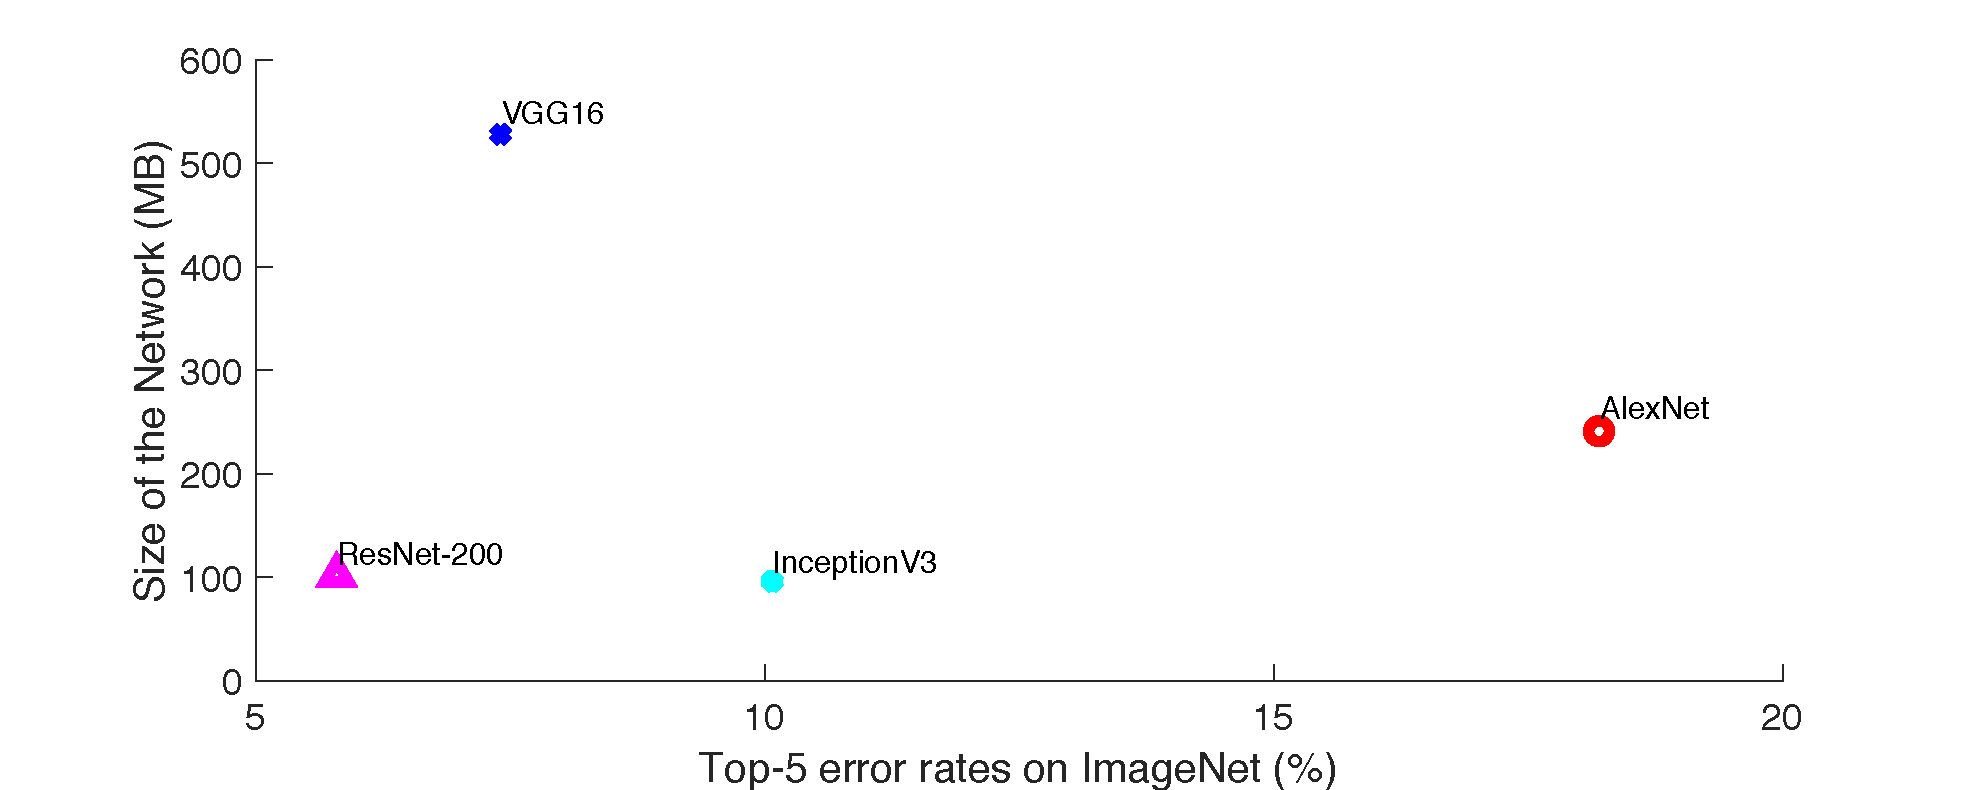
\includegraphics[width=\textwidth]{fig_network_size}
  \caption{Popular networks targeting on \textit{ImageNet ILSVRC 2012} dataset \cite{deng2009imagenet}.}
  \label{fig:network_size}
\end{figure}

While the parallelisms
offered by GPUs can be exploited to accelerate neural network training in a large scale
, deploying a network with
a large number of parameters on a memory-limited power-sensitive device becomes
increasingly difficult.
To constraint the problem space, this project focuses on
neural network inference rather than training.
There are some recent proposed algorithms, such as \textit{Deep Q Learning} \cite{Mnih}
and \textit{Asynchroous Q Learning} \cite{Mnih2016}, that require training of a
neural network on a local embedded system.
This need of executing network training in local embedded systems is still only
essential for a small set of learning algorithms.
The more appealing problem currently is how to execute network inference in
an efficient manner.
To execute network inference, although it is a simpler task than training,
mobile systems struggle to achieve a reasonable power efficiency.
Two major constraints prevent neural network inference from being applicable in real-life.
First, the large size of a neural network makes storing its parameters in embedded systems
very challenging.
For example, the \textit{AlexNet} model is over 200MB and \textit{VGG16} model is over 500MB \cite{Han15, DBLP:journals/corr/SimonyanZ14a}.
These large storage overheads post a challenge to the fundamental limit of memory size and
memory bandwidth of embedded systems.
Second, energy consumption is dominated by memory accesses \cite{Tien}, and accessing
a large number parameters of a neural network can exceed the energy envelope of
many power sensitive devices.
For instance, the battery of a smartphone struggles with running object classification using \textit{AlexNet}
in real-time for more than an hour \cite{Tien}.

To resolve the above problems, the computer architecture community is now actively
researching on novel hardware architectures for neural network inference.
Many novel custom hardware architectures
have been proposed for neural network inference \cite{chen2014dadiannao,chen2014diannao,han2016eie,han2016ese}.
Various FPGA-based accelerators have been recently applied on neural network
inference \cite{zhang2015optimizing, Nurvitadhi:2017:FBG:3020078.3021740}.
In addition, there is an increasing number of ASIC designs for deep neural
network inference \cite{han2016eie, chen2017eyeriss}.
These accelerators normally utilize a large on-chip memory and have custom computing
units to calculate matrix dot-products.
A custom accelerator is definitely beneficial for running neural network inference
efficiently, but accessing and storing the large number of parameters in the memory
is still a limit for these accelerators.

To build a hardware accelerator, the first step is to consider how to condense
the neural network to a reasonable size.
A compressed neural network is more amenable to memory-limited systems and also
reduces the energy cost of data movements.
Neural network compression is recently catching attentions and many research
works have made significant contributions in this field.
I would like to systematically summarize and evaluate state-of-art neural network compression
techniques.
These compression techniques are categorized into three groups:
pruning, regularization and quantization.
Some of these methods, such as pruning and regularization, encourage sparsity
in a neural network; in other words, these methods reduce the number of parameters
in a neural network.
Other methods, such as quantization, takes a different approach for condensing
a neural network: they reduce the number of bits required to represent a single
parameter in a neural network.
In this report, the aim is to combine several state-of-art compression techniques
to build a complete compression pipeline.
To further constraint the problem, one of the targets is to condense networks
with no test accuracy loss.
The proposed compression pipeline has achieved a compression rate of $403$x on
\textit{LeNet5} and a compression rate of $82.2$x on \textit{CifarNet}.
These compression results outperformed many existing compression techniques
by considerable margins \cite{Han15,Guo}.

\chapter{Background}

\section{Convolutional Neural Networks}
Neural networks have been biologically inspired by the actual neural systems in
human brains.
Neurons are basic units in a neural network and each neuron provides an output
based on its connections (weights) to neurons of the previous layer and an additional
offset value (bias).
A number of neurons consists a layer, and a neural network
is a layer-wise architecture.
Two types of layers are the major components in a convolutional neural networks:
fully connected layers and convolutional layers.
A fully connected layer, as its name states, has neurons that are fully connected
to all neurons in the previous layer and neurons in a single layer do not share
any connections.
However, using only fully connected layers lose particular feature information for image
recognition.
Convolutional layers requires neurons to be connected to a local region of the
previous layer for extracting specific features of a given image.
Convolutional layers normally have 3D volumes of neurons \cite{Krizhevsky}.
Convolutions leverage three important ideas: \textit{parameter sharing}, \textit{sparse interactions}
and \textit{equivariant representations} \cite{Goodfellow-et-al-2016}.
The use of small kernels reduces connections since kernels are much smaller than
inputs (\textit{sparse interactions}), and each member of the kernel is used
at every pixel of the input (\textit{parameter sharing}).
\textit{Equivariant representations} help convolutional neural networks to extract
features at each layer and sometimes even abstract features when the layer count is large.
\Cref{fig:alexnet} shows a typical neural network structure for image recognition.
The first few layers are convolutional layers followed by maxpooling layers to
extract features from images.
Maxpooling layers downsample the inputs and thus reduce the inputs' dimensionalities.
As mentioned before, these convolutional layers are all 3D volumes of neurons.
The last convolutional layer then flattens to connect to fully connected layers.
These fully connected layers, although are 2D, but normally have a large number
of neurons, for instance, the shown figure of AlexNet has 2048 neurons on its
first fully connected layer \cite{Krizhevsky}.
% Neural networks are modelled as layers of neurons, in particular, a neural network
% for image recognition normally has a few convolutional layers and a few fully
% connected layers.
A typical neural network architecture is illustrated in \Cref{fig:alexnet},
in this case, this neural network has five convolutional layers and three fully-connected
layers \cite{Krizhevsky}.
\begin{figure}[!h]
  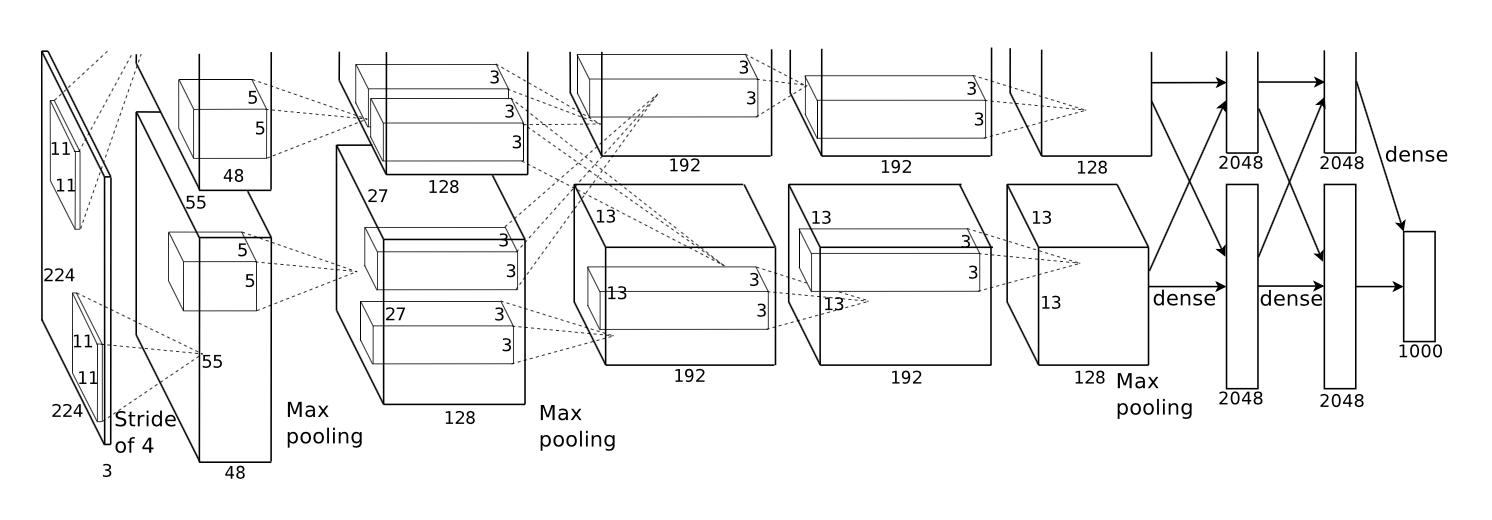
\includegraphics[width=\textwidth]{fig_alexnet.png}
  \caption{AlexNet Network Architecture \cite{Krizhevsky}.}
  \label{fig:alexnet}
\end{figure}

From a mathematical perspective, consider $w_{i}$ to be a vector of weights, $b_{i}$ to be a single biase and $x_{i}$
to be the input vector of a particular neuron $i$, this neuron generates the
following output $y_{i} = w_{i}x_{i} + b_{i}$.
This mathematical model of a single neuron feeding forward is the same as the
model of a linear classifier \cite{Mladenic}.
As illustrated in \Cref{fig:neuron}, the basic setup of neurons can be seen as
a mathematical model of actual neurons in the human brain system.
In a neural network, each output $y_{i}$ of a single neuron has to go through
an activation function, this added non-linearity becomes a key for neural network
to achieve good performance.
Popular activation functions include \textit{sigmoid} ($f(x) = \frac{1}{1+e^{-x}}$),
\textit{tanh} ($f(x) = tanh(x)$) and \textit{relu} ($f(x) = max(0,x)$).

\begin{figure}[!ht]
  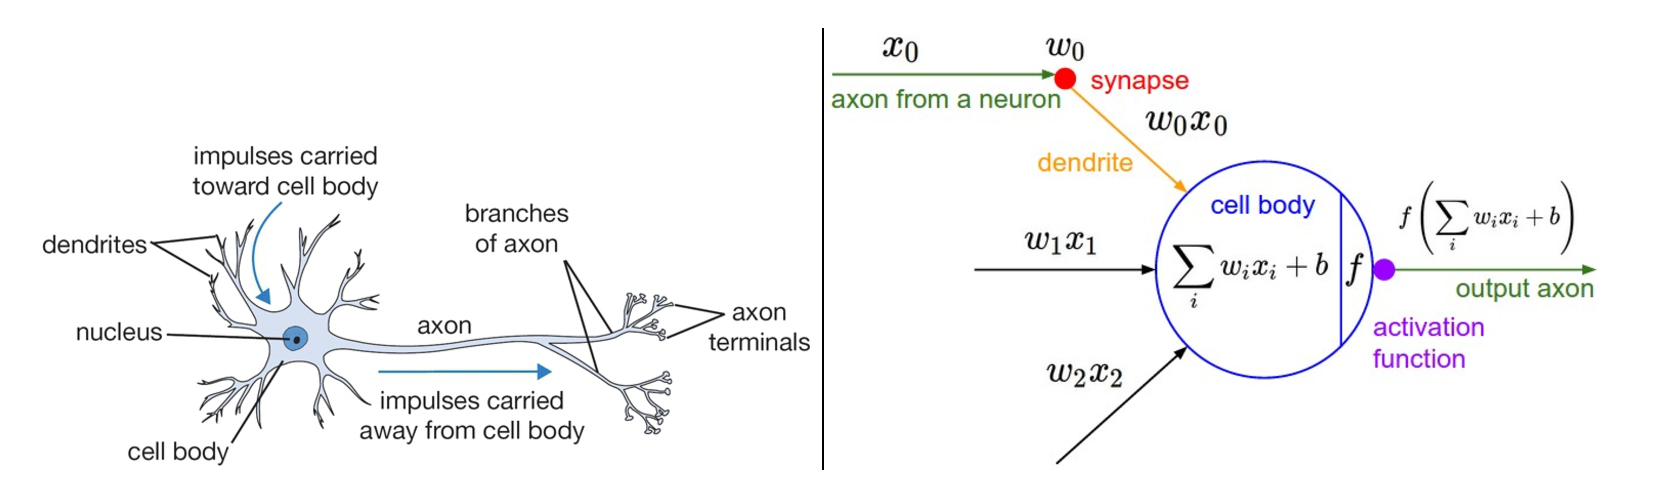
\includegraphics[width=\textwidth]{fig_neuron.png}
  \caption{Fully connected layer followed by an activation function \cite{Krizhevsky}.}
  \label{fig:neuron}
\end{figure}

Inference and training are two important operations that a
convolutional neural network can perform.
Network inference refers to a process of feeding image data to a network model and
the network produces a classification result based on its assigned parameters.
In a typical convolutional neural network, such a process only requires values from the
previous layer to be fed into the following layer, so it is also known as forward propagation.
Network training, on the other hand, performs the same forward propagation process but
has an extra process called backpropagation \cite{hecht1988theory}.
In the training stage, the predicted classification result generated from
forward propagation is compared to
a target for producing an error term (loss function).
Backpropagation works by propagating this error term from the last output layer
to the first input layer.
As shown in \Cref{equ:backprop}, $\mathbf{W_{n}}$ are weights and $\mathbf{B_n}$ are biases for
a given layer $n$, $\alpha$ is a hyperparameter called the leanring rate.
A gradient value is calculated by differentiating the loss value $L(W_n + B_n)$
with respect to each individual parameters, this first directive
determines how parameters should adjust their values for achieving a better classification
result.
The backpropogation process then updates each parameter based on their original
values and gradients, notice the learning rate $\alpha$ determines how aggressive
this update is.
% \textbf{\textit{W_{n}}} + \textbf{\textit{B_{n}}}
\begin{equation}
  \begin{aligned}
    & \mathbf{W_{n}} \leftarrow \mathbf{W_{n}}- \alpha \frac{\partial}{\partial(\mathbf{W_{n}} + \mathbf{B_n})} L(\mathbf{W_n}+ \mathbf{B_n})
  \end{aligned}
  \label{equ:backprop}
\end{equation}

The current research trend suggests convolutional neural networks will use more layers
for achieving a higher accuracy on more complicated problems \cite{Lecun1998gradient,
Krizhevsky, Coates}.

\section{Related Work}
A variety of methods have been proposed in the research community for reducing
the memory requirement of a neural network.
Although redesign the original network to a smaller network is directly beneficial, designing an efficient
network topology normally requires a large design-time.
Because efficient topologies require experimenting a set of complex connections such as
skipping layers (\textit{ResNet200}) and combing multiple parallel layers (\textit{InceptionV3})
\cite{DBLP:journals/corr/HeZRS15,DBLP:journals/corr/SzegedyVISW15}.
Another method of reducing the size of a neural network is network compression.
In general, most of compression techniques focus on the following two
paths.
\begin{enumerate}
  \item Reduce the number of parameters in a neural network.
  \item Reduce the bit-width of number representations.
\end{enumerate}
The first methodology focuses on helping a neural network to use fewer parameters.
The second path is to reduce the bit-width of each individual parameter in a
neural network, this could be done by
simply quantizing the parameters or by exploring alternative encodings or
by adding a level of indirection.
\Cref{fig:tax} provides a taxonomy of compression techniques that follow these
two paths.

\begin{figure}[!ht]
  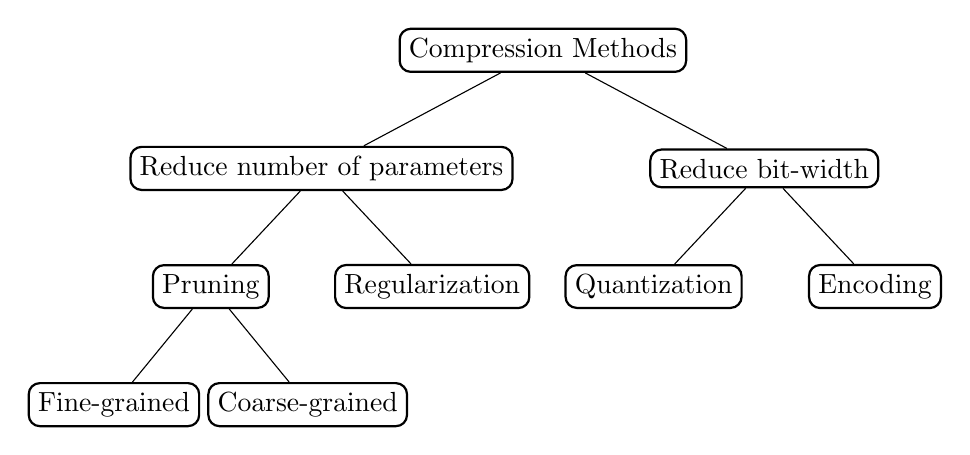
\begin{tikzpicture}[
    level 1/.style={sibling distance=16em},
    level 2/.style={sibling distance=8em},
    level 3/.style={sibling distance=7em},
    every node/.style = {shape=rectangle, rounded corners,
      draw, align=center, thick,
      top color=white}]]
    \node {Compression Methods}
      child { node {Reduce number of parameters}
        child {node {Pruning}
          child {node {Fine-grained}}
          child {node {Coarse-grained}}
        }
        child {node {Regularization}}
      }
      child { node {Reduce bit-width}
        child { node {Quantization}}
        child { node {Encoding} }
  };
  \end{tikzpicture}

  \caption{Taxonomy of compression techniques.}
  \label{fig:tax}
\end{figure}

% \begin{tikzpicture}[
%   level 1/.style={sibling distance=20em},
%   level 2/.style={sibling distance=10em},
%   every node/.style = {shape=rectangle, rounded corners,
%     draw, align=center,
%     top color=white}]]
%   \node {Compression Methods}
%     child { node {Reduce number of parameters}
%       child {node {Pruning}}
%       child {node {Regularization}}
%     }
%     child { node {Reduce bit-width}
%       child { node {Quantization}}
%       child { node {Encoding} }
% };
% \end{tikzpicture}
Network pruning has been widely used for reducing the number of
parameters in convolutional neural networks \cite{Lecun1998gradient, Hassibi, Srinivas2015}.
Pruning methods can be classified based on their granularities (\Cref{fig:tax}) \cite{mao2017exploring}.
Fine-grained pruning refers to pruning methods that delete individual weights.
Starting from \textit{LeCun et al.}, their idea is to use the second derivative
of the network's loss function to balance the predication accuracy and model complexity \cite{Lecun1998gradient}.
\textit{Hassibi et al.} proposed to add the non-diagonal elements of the
Hessian matrix into the pruning metric, this is proven to be helpful in reducing
excess degrees of freedom in the neural network model \cite{Hassibi}.
Recently, \textit{Han et al.} utilised fine-grained pruning and achieved
high compression rates on many popular convolutional neural networks \cite{Han15}.
Their pruning technique is tightly coupled with training, after every pruning process,
a retraining takes place to bring back the lost accuracies.
This class of pruning is also called \textit{Iterative pruning}.
Inspried by \textit{Han et al.'s} work, later on, \textit{Guo et al.} implemented
\textit{Dynamic network surgery} that combines fine-grained pruning with splicing.
In the splicing phase of \textit{Dynamic network surgery}, some weights that was previously pruned
away would have a chance to recover.
\textit{Dynamic network surgery} is able to prune more aggressively and achieved
better results than traditional iterative pruning \cite{Guo}.
Coarse-grained pruning, on the other hand, focus on pruning filters of convolutional
neural networks \cite{DBLP:journals/corr/LiKDSG16}.
Such coarse-grained pruning eases the design of hardware accelerators
due to regularities \cite{DBLP:journals/corr/WenWWCL16, DBLP:journals/corr/LebedevL15}.
Given the requirement of no loss of test accuracy is allowed, fine-grained pruning
normally works better than coarse-grained pruning, because the later suffers from
a structural loss by pruning away complete filters \cite{DBLP:journals/corr/LiKDSG16}.

Apart from pruning, there are other existing techniques that focus on
reducing the number of parameters of a neural network model.
Regularization focuses on encouraging sparsity of the neural network while training
the network.
It has long been known that adding $l_1$ norm and $l_2$ norm encourages
sparsities in a neural network.
However, these regularizers only restrict the magnitudes of weights and thus
induces sparsity in a less controlled manner.
\textit{Srinivas et al.} proposed to use \textit{spike-and-slab} regularizers
for achieving pruning on-the-fly with the training process \cite{Srinivas2015}.
\textit{Kang et al.} proposed a new regularizer called \textit{Shakeout}.
In \textit{Shakeout}, the activation functions are customized at each neuron.
The practical results of using \textit{Shakeout} suggest that this regularizer
induces more sparsity than traditional regularization methods.

Reducing the number of bits required to represent each individual parameter also
directly compresses a given neural network.
\textit{Han et al.} used \textit{Weights sharing} to group parameters with similar values \cite{Han15}.
\textit{Weights sharing} works like an encoding scheme and it normally considers weights in a layer-wise fashion.
For weights in each layer, a clustering algorithm is applied on these
weights to group them with various centroid values \cite{Han15}.
These centroids are encoded using a hash function.
For later inference operation, the centroid values are stored on-chip and
each weight is represented using a hash key that is normally small in terms of
bit-width.
This idea origins from \textit{HashNet} proposed by \textit{Chen et al.} \cite{chen2015compressing},
but is different from the original work since now the hash function
applies only on a trained network rather than changing the entire network architecture.
Quantization is another popular method for reducing the bit-width of individual parameters.
Fixed-point arithmetic has been confirmed to be a more energy efficient arithmetic
for neural network inference \cite{moons2016energy}.
Quantized networks, also known as low precision networks, utilizes low-precision
fixed-point arithmetic to reduce the bit-width of individual parameters in the
neural network \cite{Hubara}.
Reaching an extreme, neural networks with parameters of only 1-bit width are
known as \textit{Binarized neural networks} \cite{Courbariaux}.
\textit{Ternary weight networks}, neural networks with parameters constrained to
$1$, $0$ and $-1$, have been recently proposed and demonstrated an advance in
performance compared to  \textit{Binarized neural networks} \cite{li2016ternary}.
However, \textit{Binarized neural networks} and \textit{Ternary weight networks} normally require re-implementations to recover
its accuracy loss and thus is beyond the scope of this project.
For reducing the size of individual parameters, in this project, I will focus on
various quantization methods and \textit{Weights sharing}.

Although a large number of compressing techniques have been proposed, most of these
techniques are proposed in isolations -- they do not consider how
to combine with each other in an optimal manner.
Recently, \textit{Han et al.} firstly proposed \textit{Deep Compression} that is
a complete compression pipeline utilizing several different compression techniques.
It is possible to build a compression chain that makes use of compression techniques
from orthogonal optimization spaces.
\textit{Deep Compression} offers a large compression rate on many popular networks
combing \textit{Deterministic pruning}, \textit{Fixed-point quantization},
\textit{Weights sharing} and \textit{Huffman encoding}.
This project aims to evaluate further in this compression optimization space.
A larger number of state-of-art compression techniques, including different pruning
schemes and quantization schemes are considered for building a better compression pipeline.
In addition, this project puts a focus on developing novel pruning and
quantization strategies based on some existing compressing techniques.



\section{Experiment Setups, Datasets and Trained Networks}
In this project, I select \textit{TensorFlow} to be the implementation tool \cite{tensorflow}.
This package has python APIs that are easy to use, and \textit{CUDA} backend for
efficient GPU utilizations.
Several local GPU machines and Amazon Cloud machines are used to train the networks.

Two datasets, \textit{MNIST} \cite{lecun1998mnist} and \textit{CIFAR10} \cite{krizhevsky2014cifar},
are considered in this project.
% Due to the time limitation of this project, only two datasets are considered.
Both datasets are smaller than the popular \textit{ImageNet} dataset \cite{deng2009imagenet}.
Sine the optimization space is large and training a large network on a large dataset
is time-consuming, the \textit{ImageNet} dataset is not considered in this project.
\textit{MNIST} dataset is a relatively small dataset for experimenting ideas.
\textit{CIFAR10} dataset serves as a representative for large networks.

The first dataset, \textit{MNIST}, consists of handwritten digits.
\textit{MNIST} has a training set of $60,000$ images and a test set of $10,000$
images.
These images are a subset of the bigger \textit{NIST} dataset \cite{grother1995nist},
and all the digts in this dataset have been normalized in size and centered in
the middle \cite{lecun1998mnist}.
I used the \textit{LeNet5} model \cite{lecun2015lenet} to recognize \textit{MNIST} images.

Another dataset considered in this project is the \textit{Cifar10} dataset.
\textit{Cifar10} is a subset of the \textit{80 million tiny images dataset} \cite{torralba200880}.
The \textit{Cifar10} dataset is divided into five training batches and one test batch,
each batch contains $10,000$ images \cite{krizhevsky2014cifar}.
\textit{CifarNet} is the neural network architecture used to recognize images in the
\textit{Cifar10} dataset \cite{krizhevsky2009learning}.
It is important to note that, all these datasets are carefully designed so that
all classes are mutually exclusive.
\begin{table}[!h]
\centering
\begin{tabular}{|l|l|l|l|l|l|}
\hline
Layer			&cov1	&cov2	&fc1	&fc2 		&total\\ \hline
Params		& 0.5K		&25K	&400K	&5K		&431K\\
\hline
\end{tabular}
\caption{Number of parameters in LeNet5-431K.}
\label{tab:LeNetparam}
\end{table}

\begin{figure}[!h]
  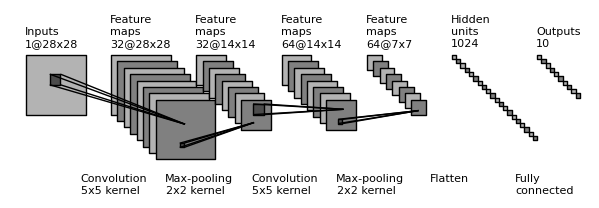
\includegraphics[width=\textwidth]{fig_mnist.png}
  \caption{LeNet5 Network Architecture}
  \label{fig:lenet5_arch}
\end{figure}

Firstly, I am using a trained \textit{LeNet5} model with 431K parameters that
has an error rate of only $0.64\%$ on the \textit{MNIST} dataset.
The original \textit{LeNet5} model proposed by \textit{LeCun et al.} has around 1000K
parameters, however, later research works all use an implementation of \textit{LeNet5}
with 431K parameters \cite{jia2014caffe, Han15, Guo}.
In this project, the 431K implementation of \textit{LeNet5} is chosen to enable a
fair comparisons to be made with published results from related research works.
The detailed information regarding the number of parameters
at each layer of this \textit{LeNet5} network is shown in \Cref{tab:LeNetparam}.
The network's architecture is shown in \Cref{fig:lenet5_arch}.
As shown in the figure, this architecture includes two convolutional layers and three fully connected
layers.

The \textit{Cifar10} dataset is larger compared to \textit{MNIST}.
A \textit{CifarNet} architecture is constructed and trained to an error rate of $18\%$.
As expected, since this larger dataset implies a harder image recognition task,
the trained model uses a larger number of parameters and more layers
to achieve a reasonable accuracy.
A graphical illustration of the \textit{CifarNet} architecture is shown in \Cref{fig:Cifarnetparam},
The \textit{CifarNet} architecture has two convolutional layers and three fully connected
layers.
The input images of the dataset now have three channels.
The number of parameters at each layer of the \textit{CifarNet} is summarized
in \Cref{tab:CifarNetparam}.

\begin{figure}[!h]
  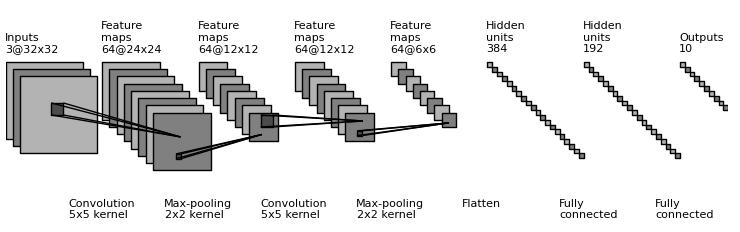
\includegraphics[width=\textwidth]{fig_cifarnet.png}
  \caption{CifarNet Network Architecture}
  \label{fig:Cifarnetparam}
\end{figure}

\begin{table}[!h]
\centering
\begin{tabular}{|l|l|l|l|l|l|l|}
\hline
Layer			&cov1	&cov2	&fc1	&fc2	&fc3 		&total\\ \hline
Params		& 4.8K		&102.4K	&885K	&74K	&2K &1068K\\
\hline
\end{tabular}
\caption{\label{tab:CifarNetparam}Number of parameters in CifarNet.}
\end{table}

\chapter{Pruning}
\label{sec:dprune}
Pruning is an effective method for reducing the redundancies in a network.
I mainly focus on fine-grained pruning methods in this project since they achieve best
compression results \cite{mao2017exploring}.
Fine-grained pruning inspects all parameters in a layer and moves away individual connections that have values
lower than a certain threshold.
Pruning is normally combined with iterative retraining so that lost accuracies caused by pruning can
be recovered directly.
In this chapter, I aim to reproduce existing fine-grained pruning techniques:
\textit{Deterministic pruning} \cite{Han} and \textit{Dynamic Network Surgery} \cite{Guo}.
At the end of this chapter, I compared the performances of various
existing fine-grained pruning strategies on selected neural network models.

\section{Deterministic Pruning}
\subsection{Pruning Both Weights and Biases}
\label{sec:prune_without_biase}
Pruning reduces the total number of parameters and finds the minimal
neural network topology, but an overly pruned network suffers from a significant
accuracy drop and even divergence \cite{Thimm}.
Consider a set of weights for a neural network of $N$ layers,
the weights can be expressed as $\{\mathbf{W_n} : 0 \leq n \leq N \}$, so that $\mathbf{W_n}$ is the
weights for a given layer $n$.
Similarly, biases are expressed as $\{\mathbf{B_n} : 0 \leq n \leq N \}$.
To represent a sparse model, a binary matrix
$\{\mathbf{M_n}: 0 \leq n \leq N\}$ for weighs and a binary
matrix $\{\mathbf{M^b_n}: 0 \leq n \leq N\}$ for biases are used to indicate connections that are kept.
For simple \textit{Deterministic pruning}, \Cref{equ:hfunc} shows how this binary mask
is computed using the weights.
An arbitrary threshold value $t_n$ is used to determine whether a certain weight
variable should be pruned away.
I use $h_n(*)$ to denote the discriminative function that produces a binary mask
matrix based on the weight matrix.
\begin{equation}
  h_n(\mathbf{W_n}^{(i,j)}) =
  \begin{cases}
    0, &\text{if } t_n < |\mathbf{W_n}^{(i,j)}| \\
    1, &\text{if } t_n \geq |\mathbf{W_n}^{(i,j)}|
  \end{cases}
  \label{equ:hfunc}
\end{equation}

The appealing question now is how to determine the threshold value $t_n$.
Instead of picking threshold values in an arbitrary fashion \cite{Han} like \textit{Han et al.} , motivated by the
implementation of \textit{Dynamic network surgery} \cite{Guo}, the
following metric is used for determining the pruning threshold $t_n$:
\begin{equation}
  t_n = u_n + c \sigma_n
  \label{equ:tn}
\end{equation}

$u_n$ is the mean value and
$\sigma_n$ is the standard deviation of the parameters in layer $n$.
In \Cref{equ:tn}, $c$ is a hyperparameter used to define how aggressive this
pruning is.
The threshold determination in \Cref{equ:tn} works better than defining an arbitrary threshold
value since threshold can be determined automatically without manually inspecting the weights
distributions.

In a sparse neural network model, weights of each layer $n$ can be easily
expressed using an element-wise product between $W_n$ and $M_n$.
The loss function, expressed as $L_n(*)$, is a metric that measures the optimisation
target of the neural network training phase.
For a given layer of $n$, the following equations set the optimization
objective:
\begin{equation}
  \begin{aligned}
    & min(L_n(\mathbf{W_n} \odot \mathbf{M_n} + \mathbf{B_n} \odot \mathbf{M^b_n})) \\
    & \mathbf{M_n} = h_n(\mathbf{W_n}) \\
    & \mathbf{M^{b}_n} = h_n(\mathbf{B_n}) \\
  \end{aligned}
  \label{equ:minfunc}
\end{equation}

For simplicity, the above optimization target is only for a given layer $n$,
a complete model optimization target is different from this single layer target.
Nonetheless, \Cref{equ:minfunc} characterizes a sparse model.
The $\odot$ symbol represents \textit{Hadamard product}, which is a binary operation
that takes two matrices and produces another matrix that has elements are the
product of the elements of the original two matrices.
In \textit{Deterministic pruning}, pruned weights cannot recover their values.
However, \textit{Deterministic pruning} occurs iteratively -- a number of weights are pruned
away at each iteration and then retraining occurs to bring back the lost test accuracy caused by pruning.
Although pruned weights cannot recover their values, other
existing weights would have a chance to re-learn the correlations between existing
connections following \Cref{equ:trainfunc} \cite{Guo}.
The weights are updated concurrently by the pruned
model with a learning rate of $\alpha$.
\begin{equation}
  \begin{aligned}
    & \mathbf{W_n} \leftarrow \mathbf{W_n} - \alpha \frac{\partial}{\partial(\mathbf{W_n} \odot \mathbf{M_n} + \mathbf{B_n} \odot \mathbf{M^b_n})} L(\mathbf{W_n} \odot \mathbf{M_n} + \mathbf{B_n} \odot \mathbf{M^b_n})
  \end{aligned}
  \label{equ:trainfunc}
\end{equation}


\Cref{fig:dist_weights} shows how pruning affects the weight distribution.
In these plots, pruned weights with a value of zero are not plotted.
The plots focus on the first fully connected layer of a \textit{LeNet5} model.
The unpruned network has weights that are normally distributed and
center at zero.
The weights spread out to both positive and negative ends, and the values of
weights are normally small.
In contrast, the second plot shows how pruned weights look like: they gather
at two centers -- leaving a blank region around zero.

\begin{figure}[!h]
  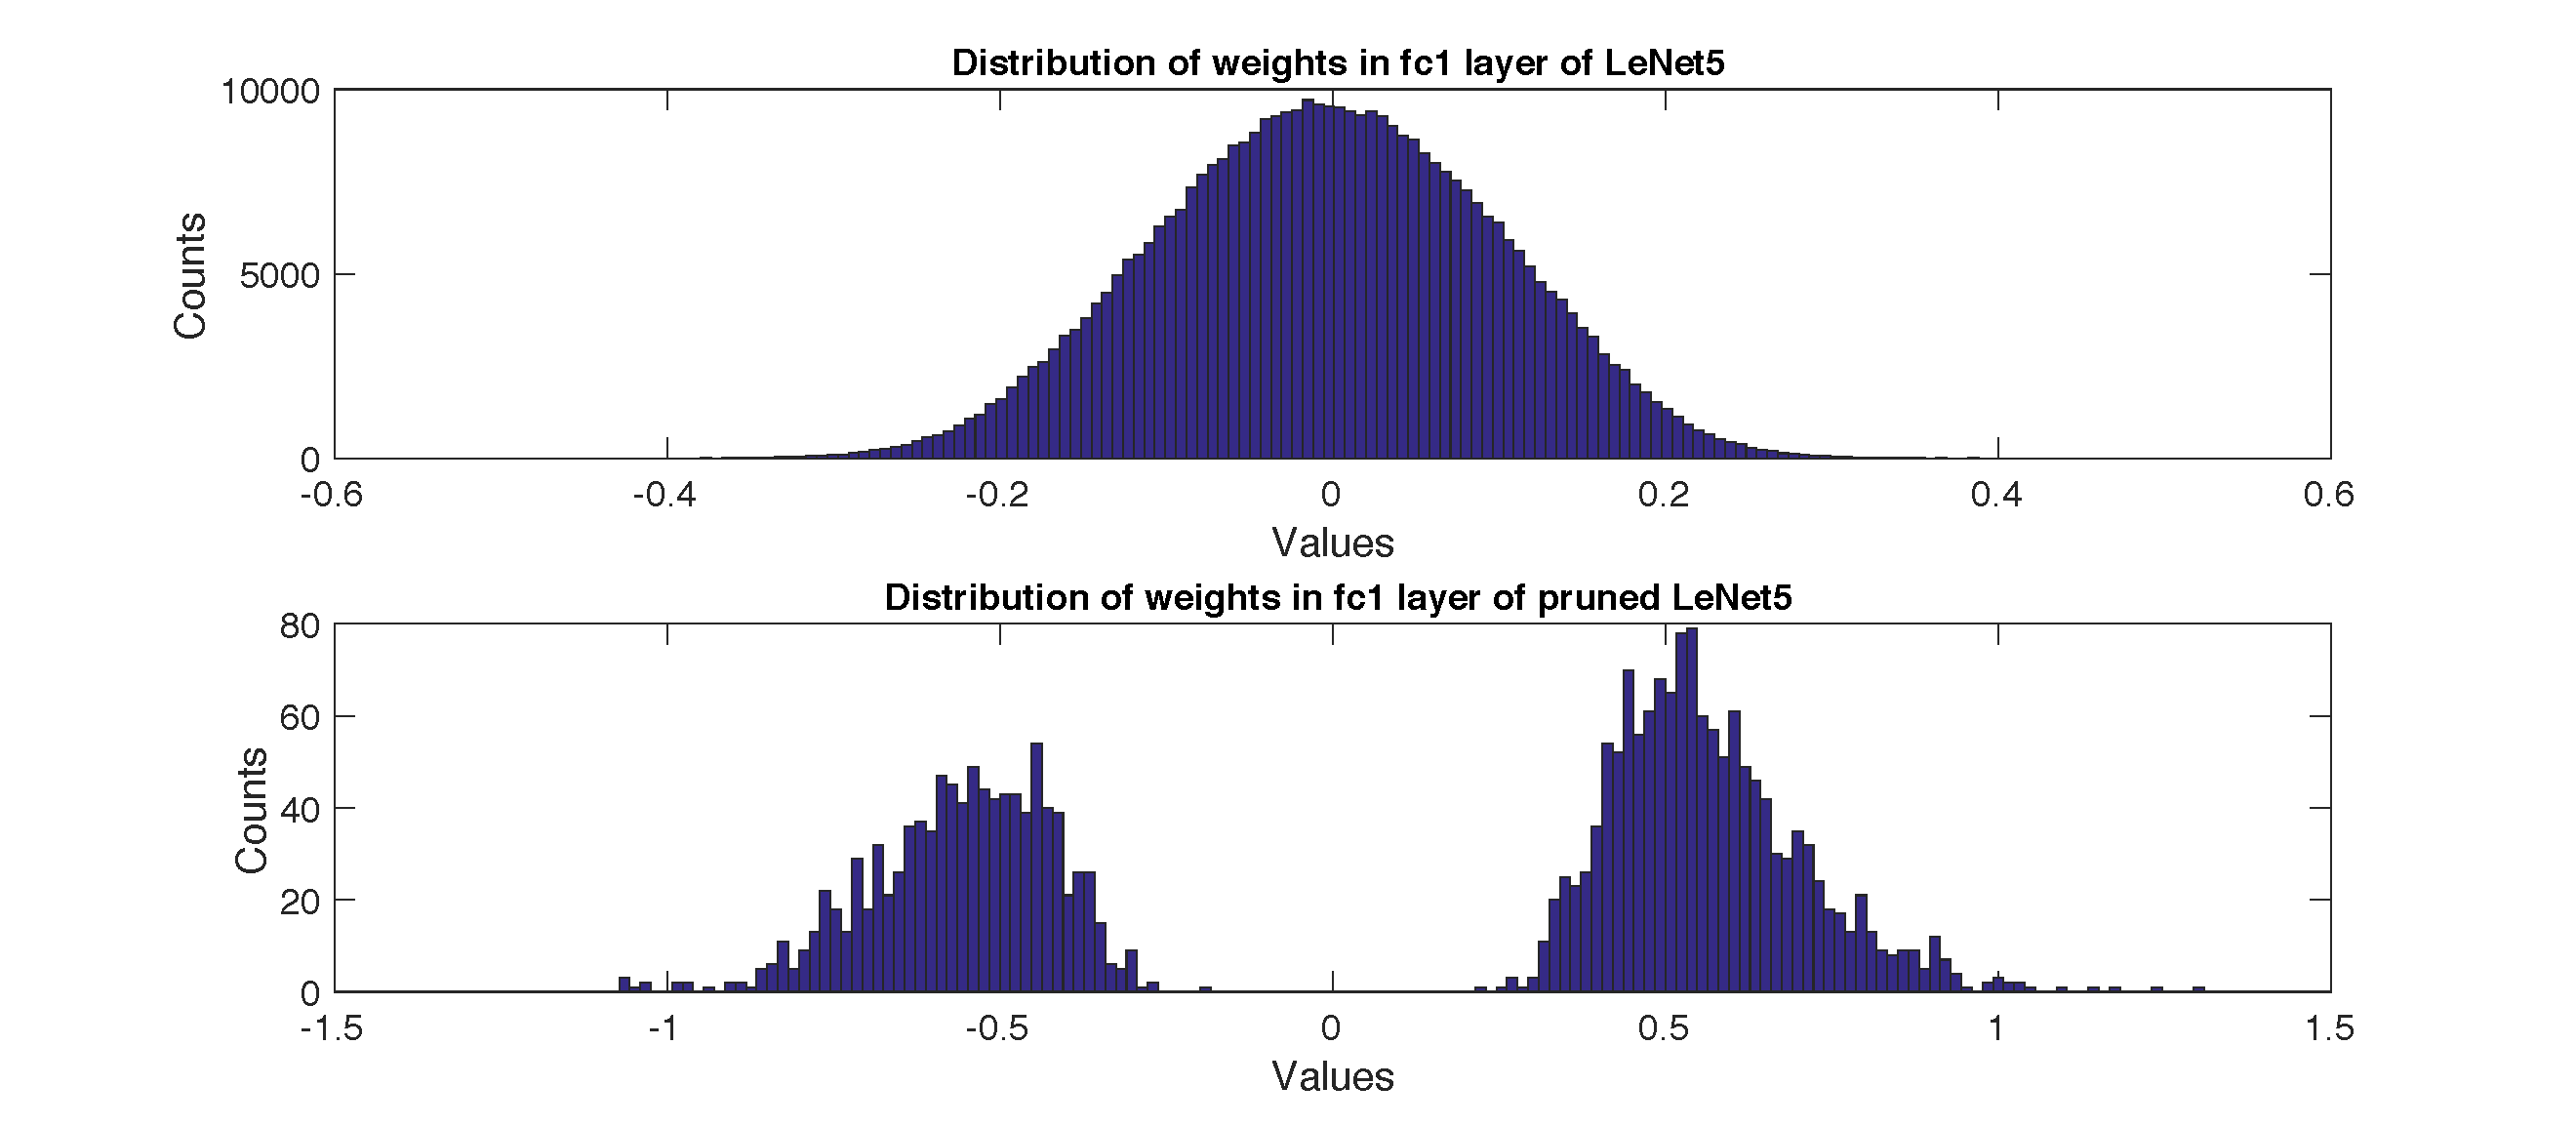
\includegraphics[width=\textwidth]{distr_weights.pdf}
  \caption{Distribution of weights in the first fully-connected layer of pruned and unpruned LeNet5}
  \label{fig:dist_weights}
\end{figure}

\begin{table}[!h]
\centering
\begin{tabular}{|l|l|l|l|l|l|}
\hline
Layer			&cov1	&cov2	&fc1	&fc2 		\\ \hline
Params		& 0.5K		&25K	&400K	&5K	\\
\hline
Prune \%	& 40\%		&80\%	&98\%	&40\%	\\
\hline
\end{tabular}
\caption{Number of parameters of pruned LeNet5-431K using \textit{Determinisitc
pruning}, and the pruning includes weights and biases.}
\label{tab:LeNetPrune}
\end{table}

\Cref{tab:LeNetPrune} shows the detailed pruning information at each layer of
the \textit{LeNet5}.
Pruning reduces the number of parameters of
\textit{LeNet5} architecture without dropping the test accuracy.
The compressed network is only $3.79\%$ of the size of the original network,
which indicates a compression rate of $26.38$x.

\Cref{tab:CifarNetPrune} shows how the pruning strategy performs on a
\textit{CifarNet}.
As shown in \Cref{tab:CifarNetPrune}, each layer of the \textit{CifarNet}
achieves a lower pruning percentage compared to \textit{LeNet5}.
This is a reasonable result, because
recognizing images in \textit{MNIST} is an easier task and the
\textit{LeNet5} network contains more redundancies than \textit{CifarNet}.

\begin{table}[!h]
\centering
\begin{tabular}{|l|l|l|l|l|l|}
\hline
Layer			&cov1	&cov2		&fc1		&fc2		&fc3		\\ \hline
Params		& 4.8K		&102.4K	&885K	&74K		&2K 	\\
\hline
Prune \%	& 30\%		&66\%	&85\%	&66\%	&30\%	 \\
\hline
\end{tabular}
\caption{Number of parameters of pruned \textit{Cifarnet} using \textit{Determinisitc
pruning}, and the pruning includes weights and biases.}
\label{tab:CifarNetPrune}
\end{table}


\subsection{Pruning Weights Only}
The number of biases of a neural network is normally small compared to
the number of weights.
More importantly, biases serve as offset values for each individual neuron,
these offsets stay invariant to different input images and could have significant
impacts on the accuracies of a neural network.
It is therefore reasonable to consider pruning only the
weights but leaving the biases unpruned.

Similar to the previous section, I compute the layer-wise optimization target
of pruning without biases in \Cref{equ:lossmin2}.
\begin{equation}
  min(L(\mathbf{W_n} \odot \mathbf{M_n} + \mathbf{B_n}))
  \label{equ:lossmin2}
\end{equation}

As the equation states, now the binary mask matrix only applies on weights variables,
the biases are kept unchanged.
\Cref{tab:LeNetPrune2} and \Cref{tab:CifarNetPrune2} show the pruning results
of \textit{LeNet5} and \textit{CifarNet} respectively.

\begin{table}[!h]
\centering
\begin{tabular}{|l|l|l|l|l|}
\hline
Layer			&cov1	&cov2	&fc1	&fc2 		\\ \hline
Params		& 0.5K		&25K	&400K	&5K		\\
\hline
Prune(a) \%	& 40\%		&80\%	&98\%	&40\%	\\
\hline
Prune(b) \%	& 51.92\%		&79.84\%	&99.38\%	&49.90\%	 \\
\hline
\end{tabular}
\caption{Number of parameters of pruned LeNet5-431K using \textit{Deterministic
pruning}. Prune(a) is pruning both weights and biases, Prune(b) is pruning weights only.}
\label{tab:LeNetPrune2}
\end{table}

\begin{table}[!h]
\centering
\begin{tabular}{|l|l|l|l|l|l|}
\hline
Layer			&cov1	&cov2		&fc1		&fc2		&fc3		\\ \hline
Params		& 4.8K		&102.4K	&885K	&74K		&2K 	\\
\hline
Prune(a) \%	& 30\%		&66\%	&85\%	&66\%	&30\%	 \\
\hline
Prune(b) \%	& 40\%		&69\%	&85\%	&69\%	&40\% \\
\hline
\end{tabular}
\caption{Number of parameters of pruned CifarNet using \textit{Deterministic
pruning}. Prune(a) is pruning both weights and biases, Prune(b) is pruning weights only.}
\label{tab:CifarNetPrune2}
\end{table}

The results of pruning without biases demonstrate itself to be a more efficient pruning
strategy compared to the previous methodology shown in \Cref{sec:prune_without_biase}.
Numerically, the compression rate of $LeNet5$ when pruned with biases is $26.38$x,
and now it increases to $37.75$x.
Similarly, the compression rate of \textit{CifarNet} has increased from $6.10$x
to $6.19$x.

To conclude, pruning with only weights gives better results and later on in this
project, all pruning methods only apply on the weights of the neural
networks.

\section{Dynamic Network Surgery}
\textit{Dynamic network surgery} is a pruning method proposed by \textit{Guo et
al.} recently \cite{Guo}.
\textit{Guo et al.} proved experimentally that \textit{Dynamic network surgery}
outperforms other existing pruning methods by considerable margins \cite{Guo}.
This method combines pruning with splicing.
Splicing refers to a procedure where some pruned weights are selected to
rejoin the network for the next pruning iteration.
The complete procedure of \textit{Dynamic network surgery} is shown in
\Cref{fig:dynamic_network_surgery}.

\begin{figure}[!h]
  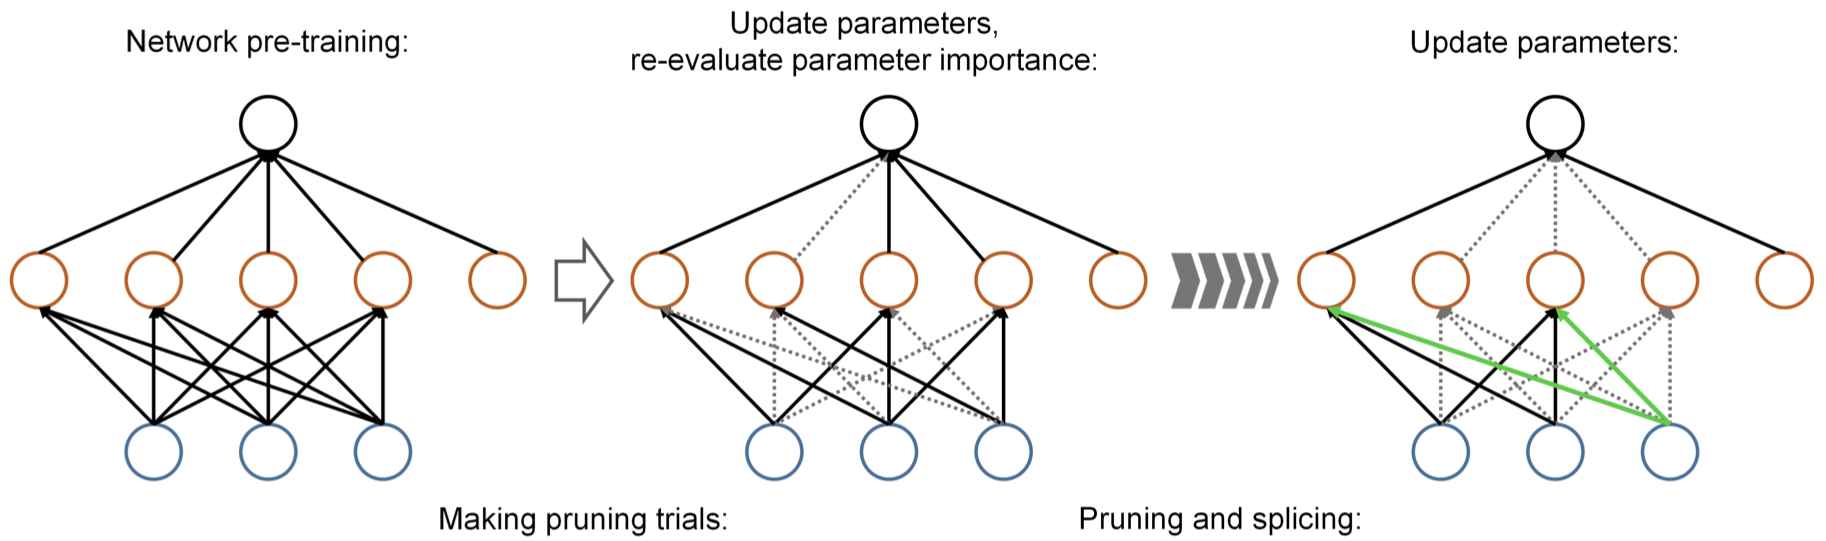
\includegraphics[width=\textwidth]{fig_dns.png}
  \caption{Mechanism of \textit{Dynamic network surgery} \cite{Guo}.}
  \label{fig:dynamic_network_surgery}
\end{figure}

In the previous sections, all pruning strategies are deterministic,
meaning that a network might suffer from an irretrievable damage once some
important weights are lost.
In contrast, \textit{Dynamic network surgery} provides a chance for pruned weights to
recover.
As shown on the rightmost plot in \Cref{fig:dynamic_network_surgery}, the green
connections are weights that have been recovered from splicing.
The splicing process minimizes the risk of causing an irretrievable damage to the
neural network.
Consider the parameters defined previously, the major difference now is on
the discriminative function:
\begin{equation}
  h_n(\mathbf{W_n}^{(i,j)}) =
  \begin{cases}
    0, &\text{if } t_{an} > |\mathbf{W_n}^{(i,j)}| \\
    \mathbf{M_n}, &\text{if } t_{an} \leq |\mathbf{W_n}^{(i,j)}| \leq t_{bn}\\
    1, &\text{if } t_{bn} < |\mathbf{W_n}^{(i,j)}| \\
  \end{cases}
  \label{equ:hfunc_ds}
\end{equation}

The discriminative function now have two threshold values, namely $t_{an}$ and
$t_{bn}$ for a given layer $n$.
Different from the previous discriminative function (\Cref{equ:tn}), for values that stay in
between two thresholds, their corresponding binary masks stay unchanged.
For weights that have absolute values larger than $t_{bn}$, their binary masks
become one which means these weights are recovered, in other words, these weights
are spliced.
Weights with absolute values smaller than $t_{an}$ are turned off.

For determining the threshold values, $t_{an}$ and $t_{bn}$,
\textit{Guo et al.} used the following equations in their code:
\begin{equation}
  \begin{aligned}
  &t_{an} = 0.9 (u_n + c \sigma_n) \\
  &t_{bn} = 1.1 (u_n + c \sigma_n)
  \label{equ:hfunc_ds}
  \end{aligned}
\end{equation}

Similar as before, \Cref{equ:hfunc_ds} made use of the mean and standard deviation
at each layer to help determine the pruning thresholds.
To test the performance of \textit{Dynamic network surgery}, this pruning method is
then applied on the two selected neural networks (\textit{LeNet5} and \textit{CifarNet}).
The pruning results of both \textit{LeNet5} and \textit{CifarNet} are displayed
in \Cref{tab:LeNetPrune3} and \Cref{tab:CifarNetPrune3} respectively.

\begin{table}[!h]
\centering
\begin{tabular}{|l|l|l|l|l|}
\hline
Layer			&cov1	&cov2	&fc1	&fc2 		\\ \hline
Params		& 0.5K		&25K	&400K	&5K		\\
\hline
Prune(a) \%	& 40\%		&80\%	&98\%	&40\%	\\
\hline
Prune(b) \%	& 51.92\%		&79.84\%	&99.38\%	&49.90\%	 \\
\hline
Prune(c) \%	& 36.54\%		&87.90\%	&99.66\%	&18.42\%	 \\
\hline
\end{tabular}
\caption{Number of parameters of pruned LeNet5-431K.
Prune(a) is \textit{Deterministic pruning} with both weights and biases,
Prune(b) is \textit{Deterministic pruning} with weights only and
Prune(c) is \textit{Dynamic network surgery}.}
\label{tab:LeNetPrune3}
\end{table}

\begin{table}[!h]
\centering
\begin{tabular}{|l|l|l|l|l|l|}
\hline
Layer			&cov1	&cov2		&fc1		&fc2		&fc3		\\ \hline
Params		& 4.8K		&102.4K	&885K	&74K		&2K 	\\
\hline
Prune(a) \%	& 30\%		&66\%	&85\%	&66\%	&30\%	 \\
\hline
Prune(b) \%	& 40\%		&69\%	&85\%	&69\%	&40\% \\
\hline
Prune(c) \%	& 53\%		&87\%	&95\%	&82\%	&26\% \\
\hline
\end{tabular}
\caption{Number of parameters of pruned CifarNet.
Prune(a) is \textit{Deterministic pruning} with both weights and biases,
Prune(b) is \textit{Deterministic pruning} with weights only and
Prune(c) is \textit{Dynamic network surgery}.}
\label{tab:CifarNetPrune3}
\end{table}

The use of \textit{Dynamic network surgery} significantly improves the results of
pruning.
The compression rate of \textit{LeNet5} is now $49.05$x, and the compression
rate of \textit{CifarNet} is $17.66$x.
In the previous section, \textit{Determnisitc pruning} only achieved
a compression rate of $37.75$x on \textit{LeNet5}, and $6.19$x on \textit{CifarNet}.
The significant increases in compression rates imply that \textit{Dynamic Network
Surgery} is a better pruning method.
Pruning happens in a non-deterministic fashion in \textit{Dynamic Network
Surgery}: if a pruned weight finds its importance at later stages of the
iterative pruning, it will have a chance to recover.
\textit{Guo et al.} proposed inspecting the values of weights as a representative
of their importance.
As shown in \Cref{equ:hfunc_ds}, if a pruned weight has a relatively large value
after retraining, it will be turned on again.

\section{Comparison to Existing Works}
\label{sec:pruning_ext_comp}
In this section, I would like to compare the implemented pruning methods to
their original implementations.

\begin{table}[!h]
  \centering
  \begin{tabular}{lllllllll}
    \hline
    Model   &Layer     &Params    &\%(\textit{Han}\cite{Han15})   &\%(\textit{Guo}\cite{Guo}) &\%(a)  &\%(b)    &\%(c)  &\%(d)\\
    \hline
    LeNet5  &cov1     &0.5K       &66\%               &14.2\%           &60\%   &48.1\%   &63.5\%   &10\%\\
            &cov2     &25K        &12\%               &3.1\%            &20\%   &20.2\%   &12.1\%   &6\%\\
            &fc1      &400K       &8\%                &0.7\%            &2\%    &0.6\%    &0.4\%    &5.05\%\\
            &fc2      &5K         &19\%               &4.3\%            &60\%   &50.1\%   &82.6\%   &5.84\%\\
            &total    &431K       &8\%                &0.9\%            &3.8\%  &2.4\%    &2.0\%    &0.89\%\\
    \hline

            &CR       &-          &12.5x               &108x          &26x     &42x       &49x      &111x\\
            &ER       &-          &0.8\%               &0.91\%      &0.64\%  &0.64\%    &0.64\%     &0.91\%\\
    \hline
  \end{tabular}
  \caption{\textit{LeNet5} pruning summary, CR is the compression
  rate, ER is the error rate.
  (\textit{Han}) is \textit{Deterministic pruning} used by \textit{Han et al.}.
  (\textit{Guo}) is the original \textit{Dynamic network surgery} implemented by \textit{Guo et al.}.
  (a), (b), (c), (d) are my implementations of various methods.
  (a) is \textit{Deterministic pruning} with weights and biases, (b) is
  \textit{Deterministic pruning} with weights only, (c) is \textit{Dynamic network surgery}, (d) is
  also \textit{Dynamic network surgery} but with the same error rate as (\textit{Guo}).}
  \label{fig:prune_org_summary}
\end{table}
\Cref{fig:prune_org_summary} shows how the original implementations of various
pruning methods compared to my implementations.
(a) is \textit{Deterministic pruning} with weights and biases, (b) is \textit{Deterministic
pruning} with weights only.
(c) is my implementation of the \textit{Dynamic network surgery} method.
(\textit{Han}) is the \textit{Deterministic pruning} strategy used by \textit{Han et al.}
in their \textit{Deep Compression} framework \cite{Han15}.
(\textit{Guo}) is the original implementation of \textit{Dynamic network surgery}
\cite{Guo}.
The first few rows show the percentages of parameters left at each layer
of a \textit{LeNet5} model.
The row named \textit{total} displays the total percentages of parameters that are left in the entire
neural network.
The row \textit{CR} shows the compression rates achieved using various techniques and
\textit{ER} illustrates the error rates of the pruned networks.
The compression rates achieved in my implementations are generally better than \textit{Han et al.'s}
both in terms of compression rate and test accuracies.
Comparing to the original implementation of \textit{Dynamic network surgery} ((\textit{Guo})),
(c) shows a smaller compression rate but also lower error rate.
Since the targeting network and dataset are the same, this drop in compression
rate can be seen as a trade-off between compression rate and error rate.
When I choose to tolerate an error rate of $0.91\%$,
as shown in (d), the compression rate reaches $111$x, which is very close to the original implementation proposed by
\textit{Guo et al.} ($108$x).

\begin{table}[!h]
  \begin{tabular}{llllll}
    \hline
    Model   &Layer     &Params    &(a)  &(b)    &(c)  \\
    \hline
    CifarNet  &cov1     &4.8K     &70\%   &60\%   &47\% \\
            &cov2     &102.4K     &34\%   &31\%   &13\% \\
            &fc1      &885K       &15\%   &15\%   &5\% \\
            &fc2      &74K        &34\%   &31\%   &18\% \\
            &fc3      &2K         &70\%   &60\%   &74\% \\
            &total    &1068K      &18.5\%  &17.9\%  &7.0\% \\
    \hline

            &CR       &-          &5.41x   &5.58x  &14.3x \\
            &ER       &-          &18\%   &18\%  &18\% \\
    \hline
  \end{tabular}
  \centering
  \caption{\textit{CifarNet} pruning summary, CR is the compression
  rate, ER is the error rate. (a) is \textit{Deterministic pruning} with weights and biases, (b) is
  \textit{Deterministic pruning} with weights only, (c) is \textit{Dynamic network surgery}.}
  \label{fig:cifar_prune_org_summary}
\end{table}
\Cref{fig:cifar_prune_org_summary} shows the pruning results on \textit{CifarNet},
all the pruning methods are implemented by myself.
(a) is \textit{Deterministic pruning} with weights and biases, (b) is \textit{Deterministic
pruning} with only weights.
(c) is my implementation of the \textit{Dynamic network surgery} method.
\textit{Han et al.} and \textit{Guo et al.} do not provide results for \textit{CifarNet}.
Nonetheless, this comparison demonstrates that \textit{Dynamic network surgery}
is superior to other pruning strategies.

In this section, by comparing various pruning strategies, two important observations can be
summarized.
First, biases of a neural network should not be pruned since they are only offset
values of each neuron.
Second, \textit{Dynamic network surgery} is proven to have the best performance.
Intuitively, the splicing technique allows recovering of pruned weights, which helps
to search more exhaustively for a minimal network topology.

\chapter{Optimized Pruning Strategies}
In this chapter, I will mainly describe two novel pruning strategies.
The first proposed pruning technique is called \textit{Gradient profiling},
this method benefits pruning with limited retraining resources.
The second method is \textit{Regularization aided pruning}.
By putting extra regularization terms into the cost function of a neural network,
later in this
chapter, I demonstrate that regularizers encourage sparsity of a neural network and thus
induce better pruning results.

\section{Gradient Profiling}
All pruning methods in the previous chapter only focus on pruning parameters based
on absolute values.
These implementations, however, have two problems.
First, weights with small absolute values
are pruned, but it is possible for a weight with small absolute value to stay at an important location
so pruning it might have a large impact on accuracy.
Second, large retraining time is allowed.
Consider an epoch to be a complete traverse of the training dataset.
\textit{LeNet5} is allowed to a maximum retraining of $200$ epochs, and
\textit{CifarNet} is allowed to have $300$ epochs.
The number of epochs allowed for retraining is identical to the number of epochs
spent in training the unpruned baseline models.
In this section, I would like to propose a new method called \textit{Gradient profiling}
for finding weights that are small but important for test accuracies using
limited retraining resources.

\subsection{Method Description}
Pruning with \textit{Gradient profiling} is nearly identical to \textit{Dynamic
network surgery},
apart from that it inspects the gradient changes for one epoch.
The reason for inspecting all gradients of one epoch is to find enough
observations
on the entire training dataset.
The description of the method is illustrated in \Cref{fig:gp_mech}.

% \begin{figure}[!h]
%   \centering
%   \begin{tikzpicture}[thick]
%     \node[draw,box] (a) {\begin{tabular}{c} Phase 1: \\Train the pruned \\ model for one epoch \end{tabular}};
%     \node[draw,box,right=1cm of a] (b) {\begin{tabular}{c} Phase 2: \\ Profile the gradients\end{tabular}};
%     \node[draw,box,right=1cm of b] (c) {\begin{tabular}{c} Phase 3: \\Recover pruned weights \\with large gradients \end{tabular}};
%
%     % \node[draw,box,left=1cm of c] (d) {\begin{tabular}{c}Recover pruned weights \\with large gradients\end{tabular}};
%     \draw[ultra thick,->] (a) -- (b);
%     \draw[ultra thick,->] (b) -- (c);
%     % \draw[ultra thick,->] (c) -- (d);
%   \end{tikzpicture}
%   \caption{\textit{Gradient Profiling}.}
%   \label{fig:gp_mech}
% \end{figure}
\begin{figure}[!h]
  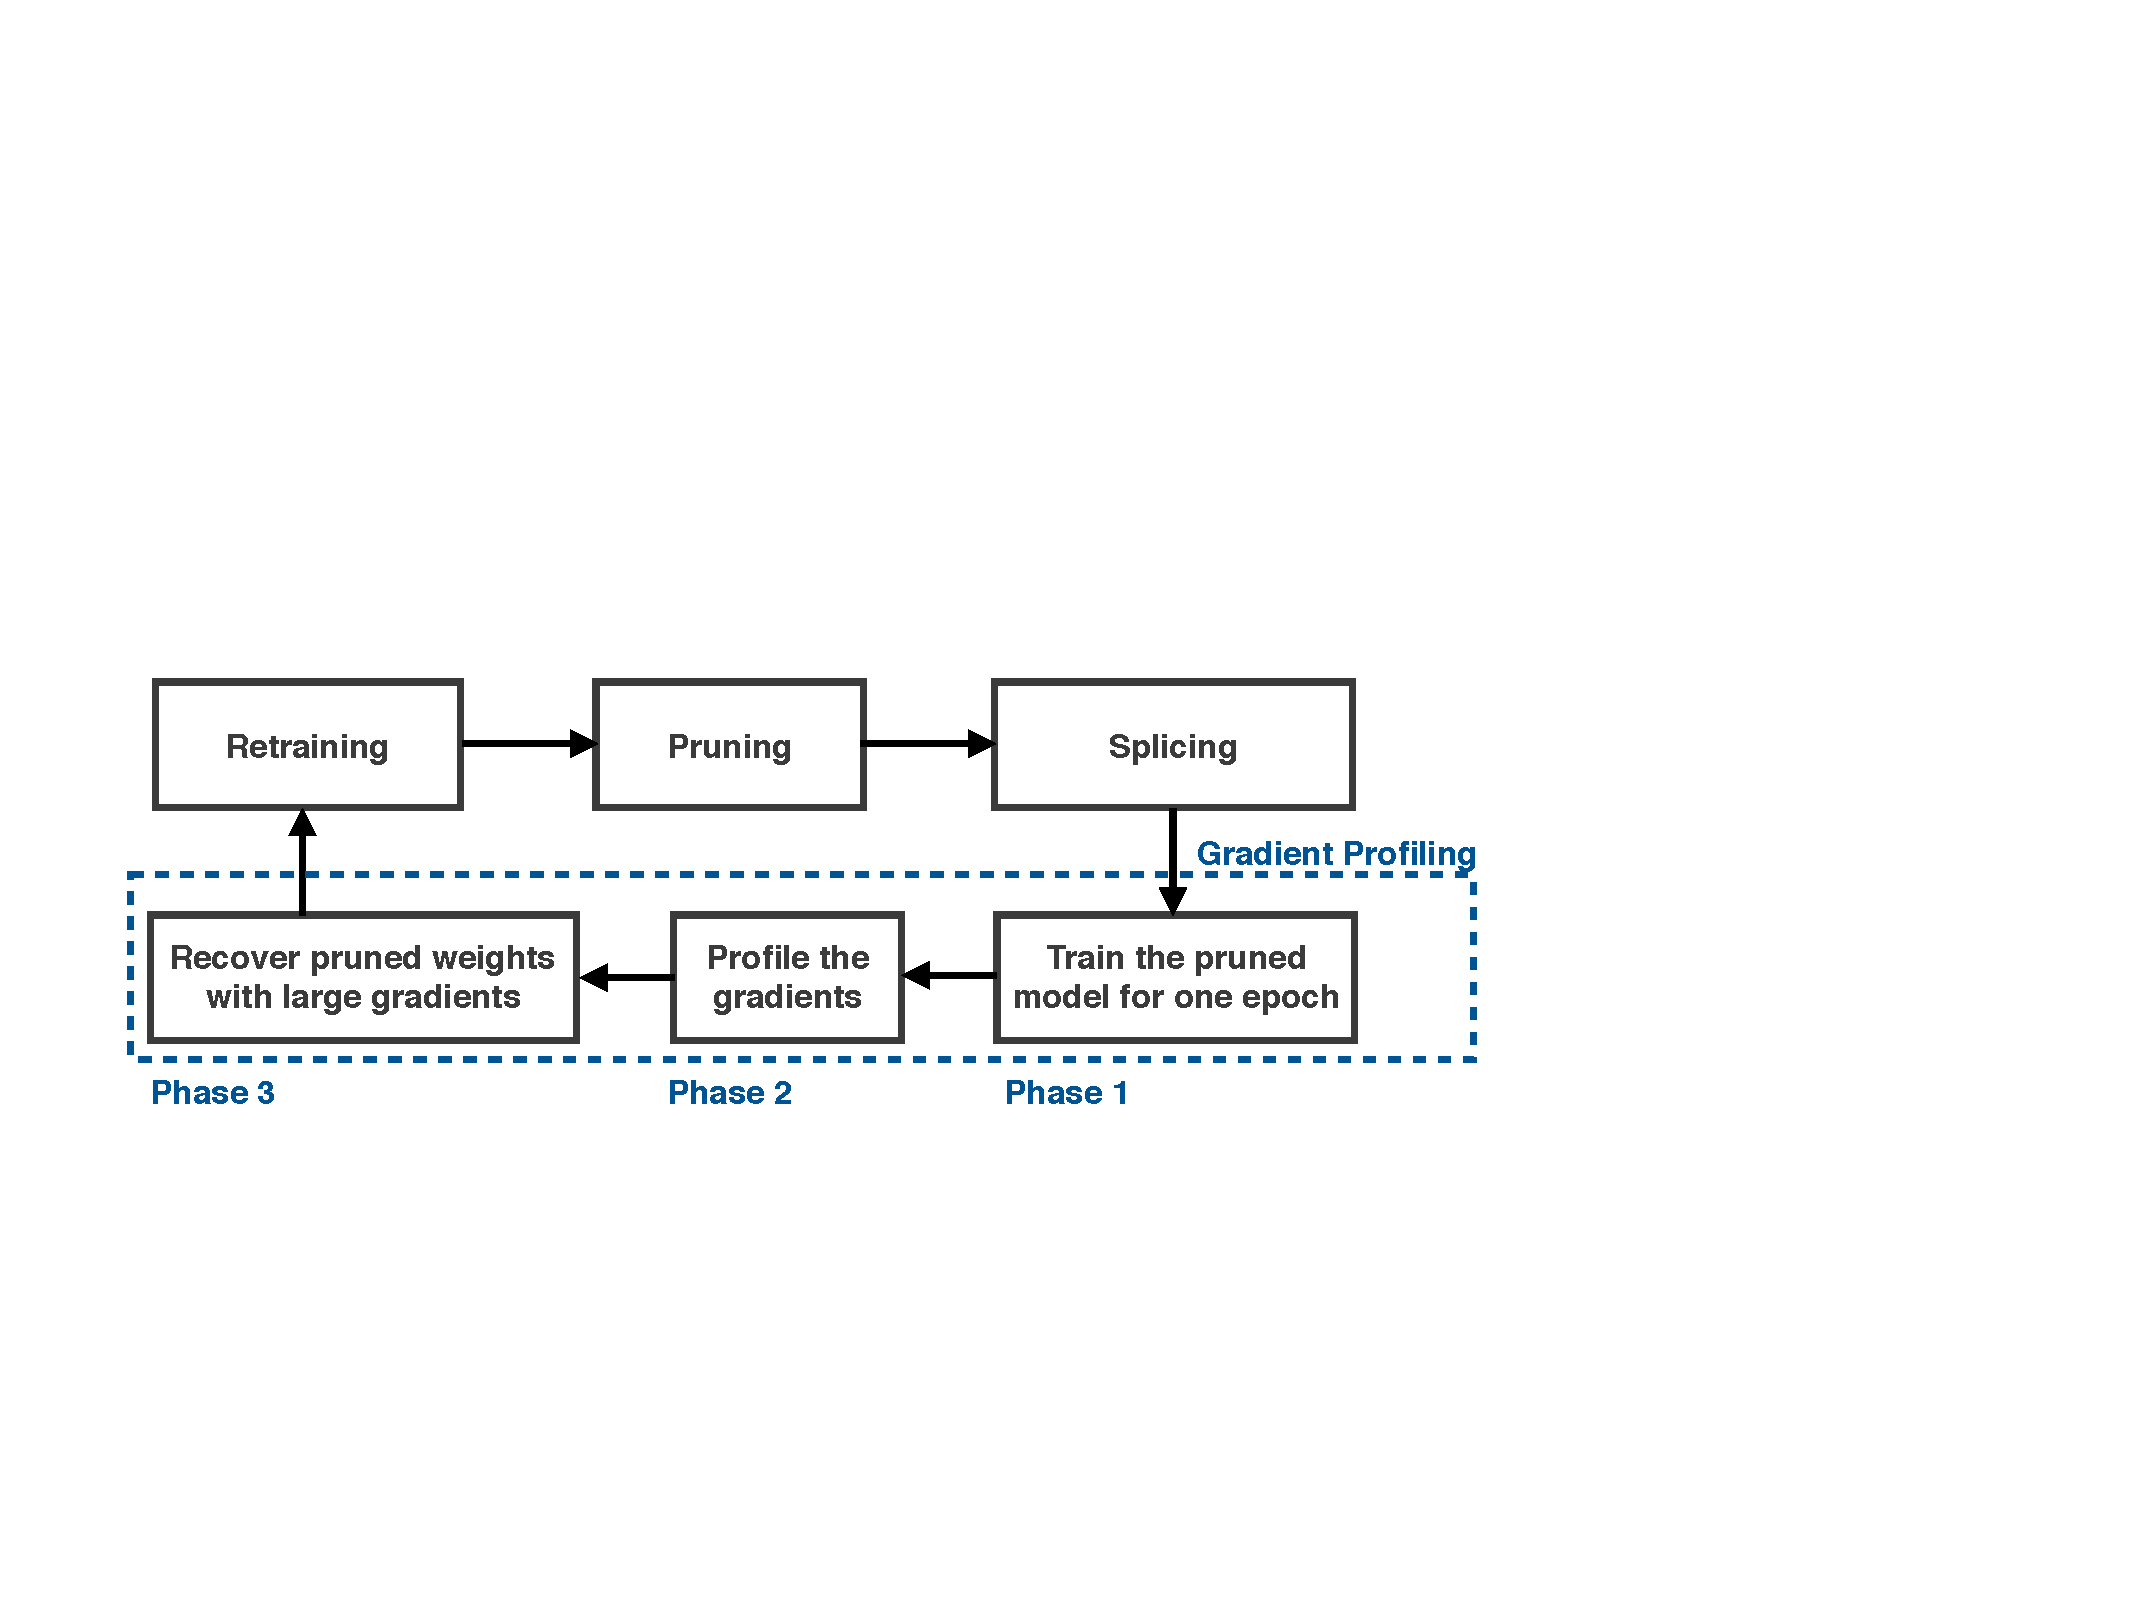
\includegraphics[width=\textwidth]{fig_gp_mech.pdf}
  \caption{Pruning with \textit{Gradient profiling}. The top row is identical to
  \textit{Dynamic network surgery}, the second row is the three phases of
  \textit{Gradient profiling}}
  \label{fig:gp_mech}
\end{figure}
The \textit{Gradient profiling} part is broken down into three phases, in the first phase, a pruned neural
network is trained only for one epoch.
The second phase collects the gradients from that one epoch training.
The third phase is to recover pruned weights based on profiled gradients data.
The amount of pruned weights that are recovered is controlled by a arbitrarily defined
hyperparamter.
In this section, the amount of recovered weights is equal to $10\%$ of the
total weights remained.
The hypothesis is that the gradients of a network serve as indications for
weights importance.
If an important weight is pruned away, the neural
network would keep passing this weight a large gradient.
Later in the gradient profiling mechanism, pruned weights with large gradients
are recognized as important weights and recovered.

From a mathematical point of view, let $\{\mathbf{G_n}: 0 \leq n \leq N\}$ to represent the
profiled gradients from phase 2 in \Cref{fig:gp_mech}.
A discriminative function $h_{gn}(*)$ is used to determine a new mask $\{\mathbf{GM_{n}}: 0 \leq n \leq N\}$
for each layer.
\begin{equation}
  \mathbf{GM_n} = h_{gn}(\mathbf{G_n}^{(i,j)}) =
  \begin{cases}
    0, &\text{if } t_{gn} < |\mathbf{G_n}^{(i,j)}| \\
    1, &\text{if } t_{gn} \geq |\mathbf{G_n}^{(i,j)}|
  \end{cases}
  \label{equ:gmfunc}
\end{equation}

$t_{gn}$ is a threshold value determined arbitrarily, as mentioned before,
the number of weights recovered from this \textit{Gradient profiling} process
is equal to a tenth of the unpruned weights.
As the number of unpruned weights keep decreasing during the iterative pruning
process, the amount of weights recovered from \textit{Gradient profiling} would
keep decreasing as well.
The loss function therefore becomes:
\begin{equation}
  \begin{aligned}
    & min(L_n(\mathbf{W_n} \odot (\mathbf{M_n} + \mathbf{GM_n}) + \mathbf{B_n}))
  \end{aligned}
  \label{equ:minfuncgp}
\end{equation}

This optimization target now embraces \textit{Gradient profiling}.
Notice the optimization target has a term -- $\mathbf{W_n} \odot (\mathbf{M_n} + \mathbf{GM_n})$.
The elements in $(\mathbf{M_n} + \mathbf{GM_n})$ can only be $1$ or $0$, because only pruned weights can be reactivated to one in $GM_n$
and pruned weights are zeros in $\mathbf{M_n}$.
The training strategy follows the same change:
\begin{equation}
  \begin{split}
    \mathbf{W_{n}} \leftarrow & \mathbf{W_{n}} - \alpha \frac{\partial}{\partial(\mathbf{W_n} \odot (\mathbf{M_n} + \mathbf{GM_n}) + \mathbf{B_n})}  \\
    & L(\mathbf{W_n} \odot (\mathbf{M_n} + \mathbf{GM_n}) + \mathbf{B_n})
  \end{split}
  \label{equ:trainfuncgp}
\end{equation}

Follow the same setup as before, $\alpha$ is the learning rate and \Cref{equ:trainfuncgp}
shows how weights are updated when both masks are applied.



\subsection{Gradient Profiling and Retraining}
To fully understand the effect of \textit{Gradient profiling}, I would like to
compare it to \textit{Dynamic network surgery} on various levels of retraining.
It is common to combine pruning methods with retraining, however, some researchers
argue that retraining takes a significant amount of time and thus should be
avoided \cite{molchanov2016pruning}.
So, in this section, I consider the following three retraining strategies:
\begin{enumerate}
  \item No retrain after pruning.
  \item Retrain for 10 epochs after pruning.
  \item Retrain for 300 epochs after pruning.
\end{enumerate}

\Cref{fig:gpvsds_noretrain} is the results when both
\textit{Gradient profiling} and \textit{Dynamic network surgery} are
applied on \textit{LeNet5} without any retraining.
The horizontal axis displays the amount of weights that are left compared to the original
network as a ratio.
For instance, $0.4$ means $40\%$ of the parameters are kept and the other $60\%$
are pruned away.
The vertical axis shows test accuracies when the network is compressed to
various sizes.
The dashed line represents \textit{Gradient profiling pruning} and the solid
line is \textit{Dynamic network surgery}.
As expected, because of the fact that some important weights are recovered by
\textit{Gradient profiling}, it shows a greater test accuracy than \textit{Dynamic network surgery}
when the size of the neural network is compressed below $0.4$ of its original size.
When the size of the neural network is relatively large (size above $0.5$),
the loss of test accuracies are not apparent and therefore both methods show
similar performances.

\begin{figure}[!h]
  \centering
  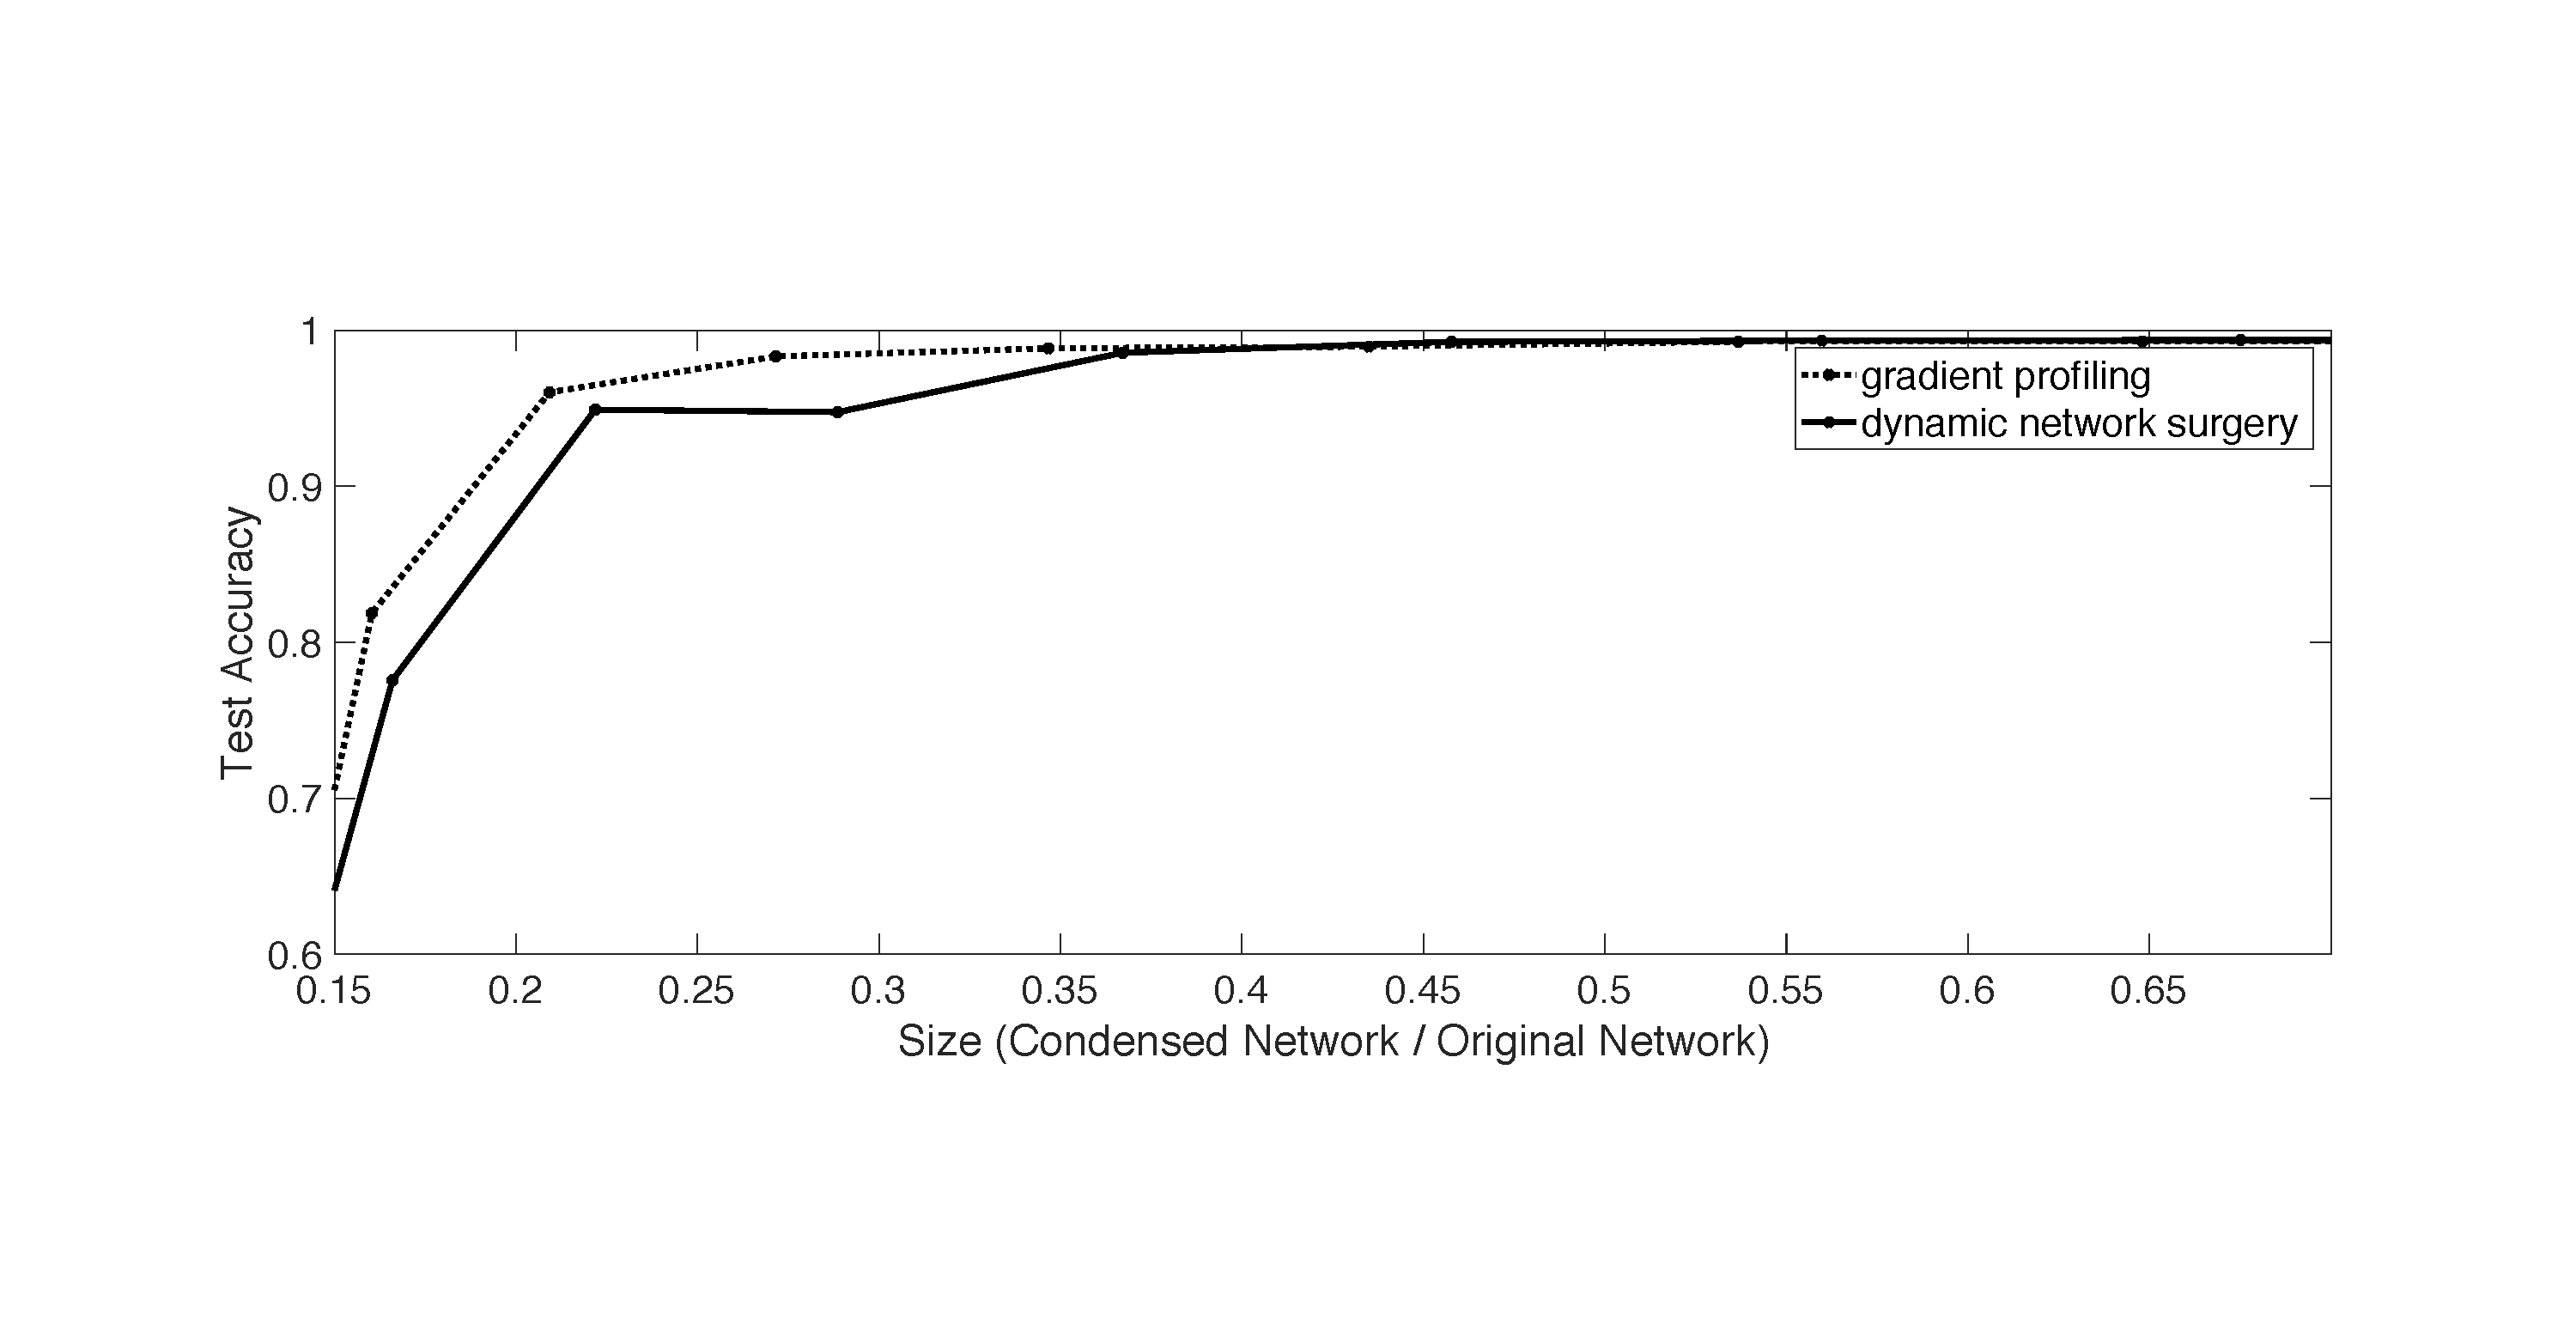
\includegraphics[width=\textwidth]{gradient_profile_noretrain.pdf}
  \caption{\textit{Gradient profiling} and \textit{Dynamic network surgery}
  without retraining. The figure shows how various compressions affect test
  accuracies.}
  \label{fig:gpvsds_noretrain}
\end{figure}

As mentioned previously, retraining recovers the test accuracies by forcing
the remaining parameters to learn to adapt with each other.
However, the amount of time spent on retraining is a major drawback of this method.
It is interesting to observe how pruning strategies are combined with \textit{limited retraining}.
I define \textit{limnited retraining} as a concept that only a very small number
of retraining epochs are allowed after pruning.
In this case, I pick to retrain only 10 epochs after pruning.
Two different pruning methods, \textit{Gradient profiling} and
\textit{Dyamic network surgery}, are considered and compared on the \textit{LeNet5} model.
\Cref{fig:gpvsds_10retrain} shows the results when 10 epochs of retraining
is applied.
As expected, the test accuracy of \textit{Gradient profiling} drops at a slower
rate compared to \textit{Dynamic network surgery}.
It is clear that between the size of $0.2$ and $0$, the test accuracies of
\textit{Gradient profiling} is significantly higher.

\begin{figure}[!h]
  \centering
  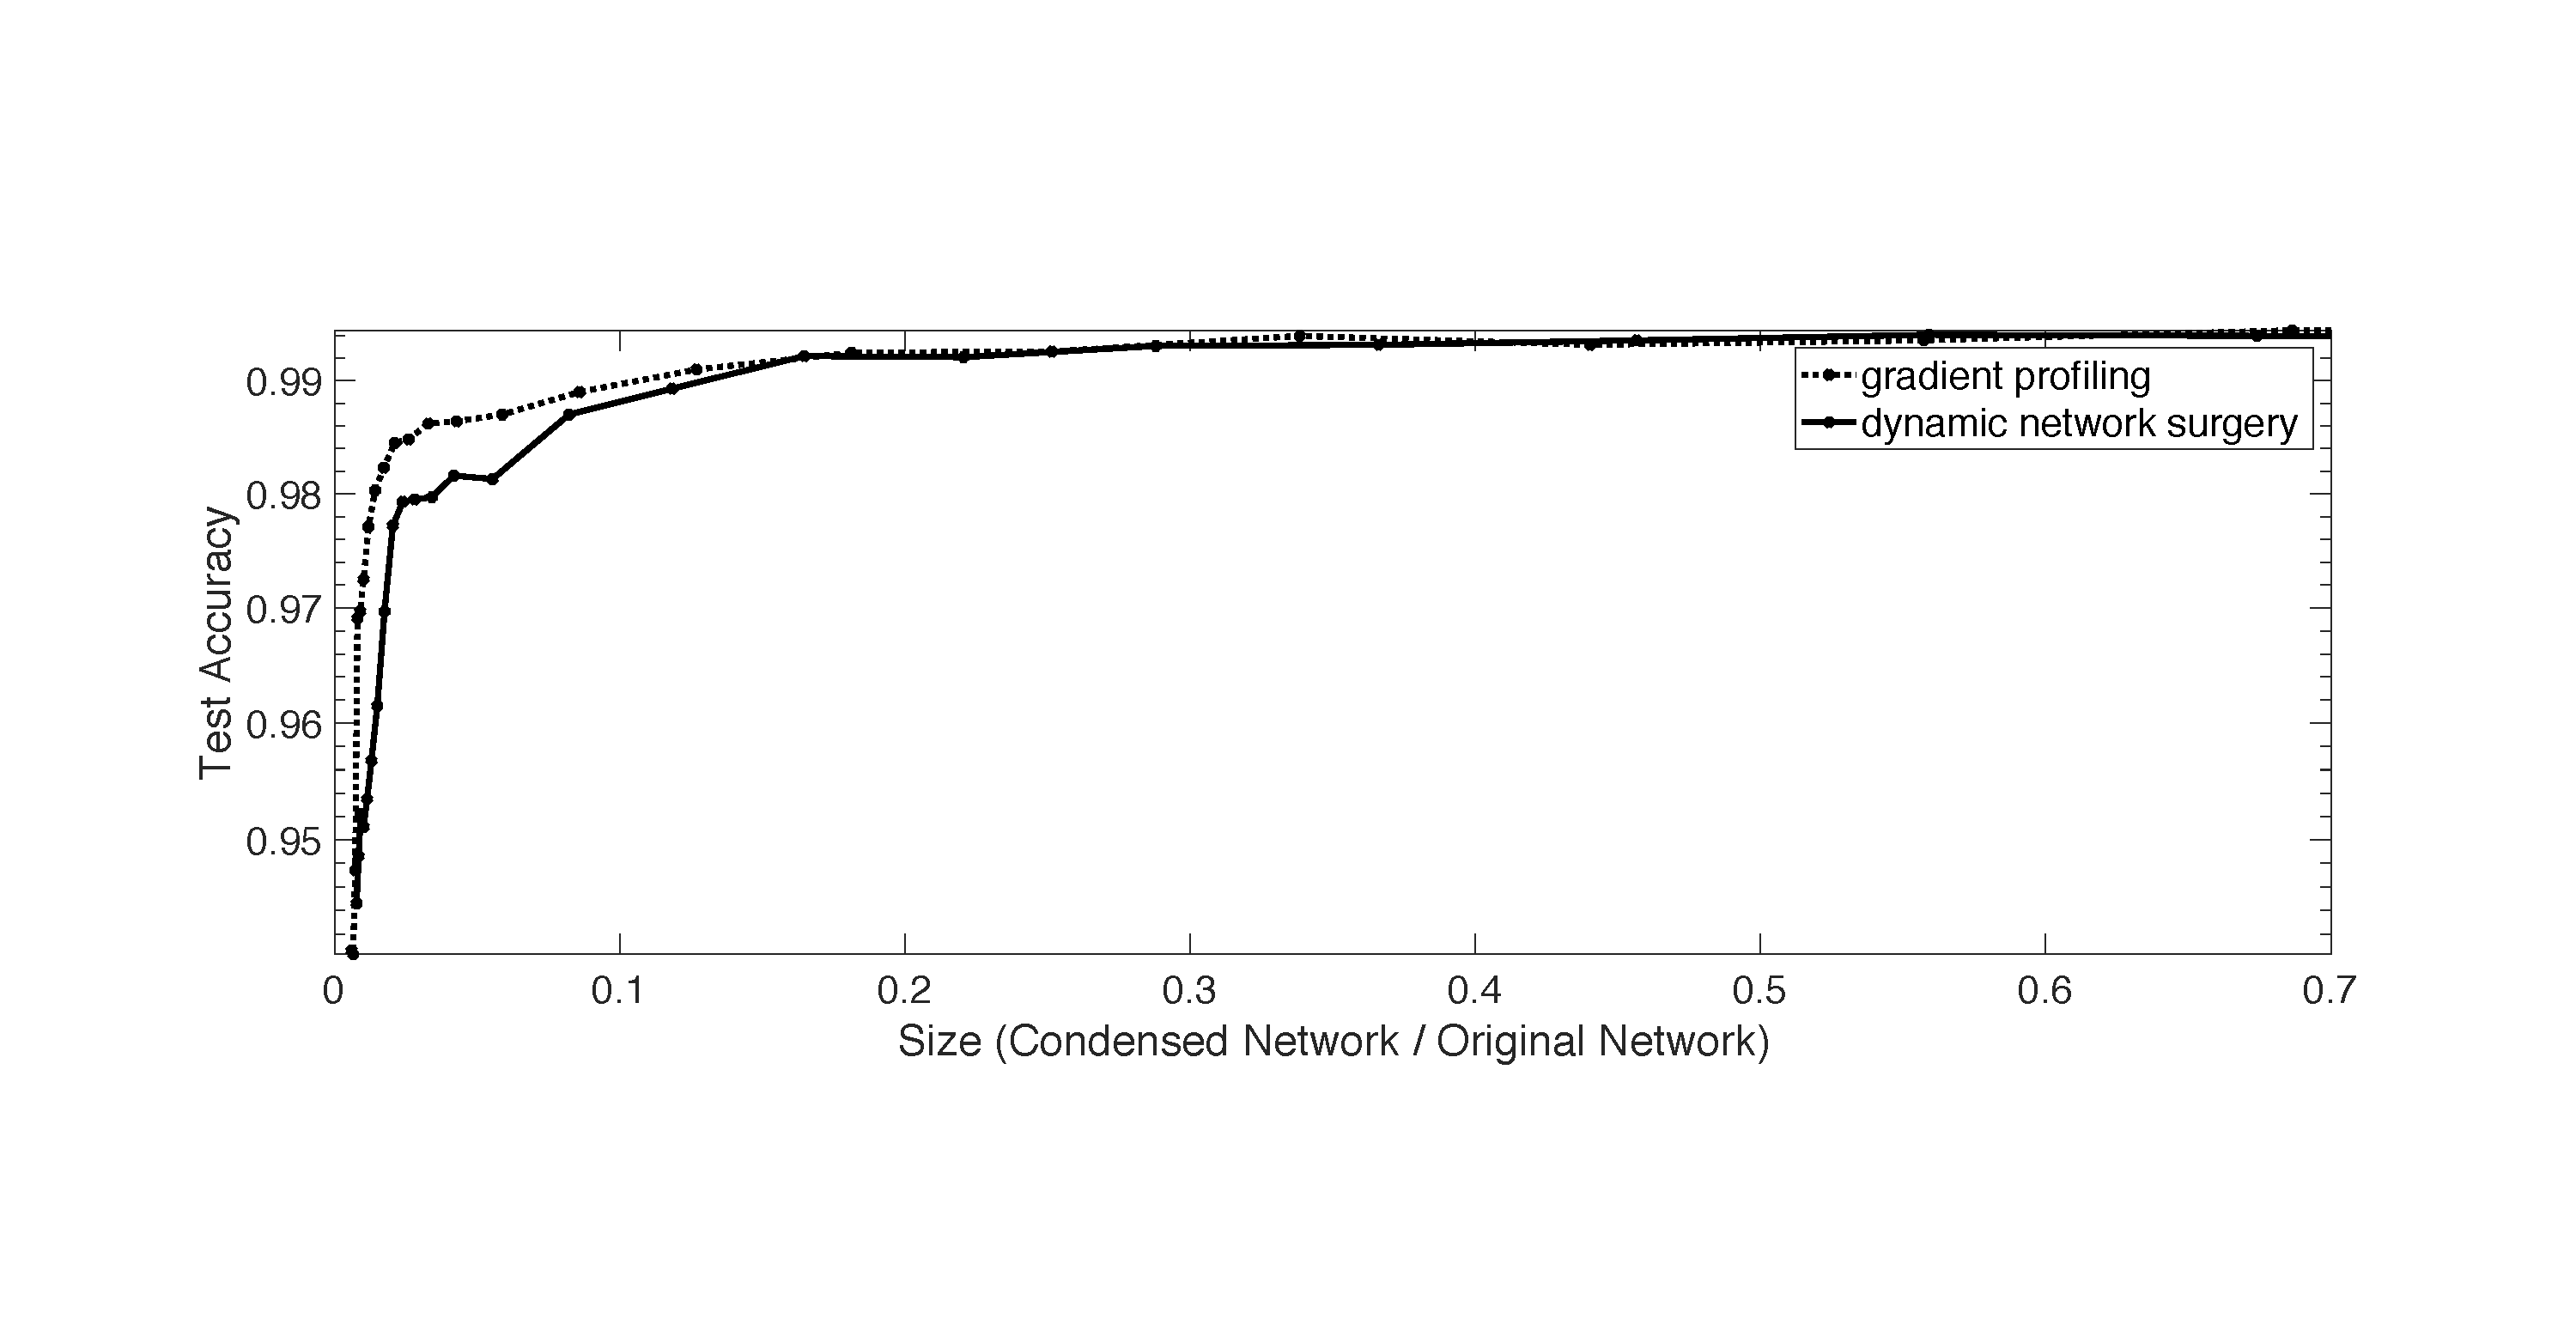
\includegraphics[width=\textwidth]{gradient_profile_10epoch.pdf}
  \caption{\textit{Gradient profiling} and \textit{Dynamic network surgery}
  with 10 epochs retraining. The figure shows how various compressed sizes affect test
  accuracies.}
  \label{fig:gpvsds_10retrain}
\end{figure}

Finally, I combine pruning with retraining of 300 epochs, and tested them
on \textit{LeNet5}.
\Cref{tab:LeNetPrunegp} shows the pruning results when using \textit{Gradient profiling}.
The compression rate is $48$x, which is slightly lower than the compression rate
of \textit{Dynamic network surgery} ($49$x).
This proves that, if retrained to convergence, \textit{Gradient profiling} is not
superior to \textit{Dynamic network surgery}.
The large amount of retraining time give weights the ability to learn to adapt with
each other.
Especially for \textit{Dynamic network surgery}, incorrect pruning has a chance
to be recovered, which gives parameters a larger chance to learn to co-adapt with
each other.
The large weights now have enough time to learn , and
previously important small weights might lose their importance because large valued
weights have already had enough time to adjust their values.
\begin{table}[!h]
\centering
\begin{tabular}{|l|l|l|l|l|}
\hline
Layer			&cov1	&cov2	&fc1	&fc2 		\\ \hline
Params		& 0.5K		&25K	&400K	&5K		\\
\hline
Prune(a) \%	&  44.20\%		&91.08\%	&99.31\%	&28.87\%	 \\
\hline
Prune(b) \%	& 36.54\%		&87.90\%	&99.66\%	&18.42\%	 \\
\hline
\end{tabular}
\caption{Number of parameters of pruned LeNet5-431K.
Prune(a) is \textit{Gradient profiling}, Prune(b) is \textit{Dynamic Network Surgery}.}
\label{tab:LeNetPrunegp}
\end{table}

To summarize, \textit{Gradient profiling} can be a very efficient pruning strategy
when retraining resource is limited.
Its enhancement on compression rate becomes limited if long retraining time is allowed.
In this project, since the topic is to construct a compression pipeline that achieves
the best compression rate, I used \textit{Dynamic network surgery} rather than
\textit{Gradient profiling} in later sections.
However, the importance and effectiveness of \textit{Gradient profiling} under
limited retraining resources still worth further evaluations.

\section{Regularization Aided Pruning}
Regularization methods are popular for preventing the neural networks from
overfitting.
Some regularization methods, such as $l_1$ norm, $l_2$ norm and \textit{Shakeout},
achieve regularization by encouraging sparsities in the model.
The use of regularizers leads to a sparse model, and this might benefit the pruning
process.
\textit{Han et al.} previously showed how to combine regularization with
\textit{Deterministic pruning} \cite{Han}, but the use of regularizers is absent
in \textit{Dynamic Network Surgery} \cite{Guo}.
In this section, I would like to investigate how regularization could
be combined with \textit{Dynamic Network Surgery}.
\subsection{$l_1$ and $l_2$ Norms}
$l_1$ and $l_2$ norms, also known as least absolute errors (LAE) and least squares
respectively, are popular regularization terms that could be appended to a
neural network's cost function \cite{nie2010efficient}.
Mathematically, the $l_p$ norm of a given vector $v$ is:
\begin{equation}
    ||v||_p = (\sum_{i=1}^{n}|v_i|^p)^{\frac{1}{p}}
\end{equation}
$l_1$ and $l_2$ norms have been proven to be robust to outliers in
data and also encourages sparsity via training \cite{nie2010efficient}.
The intuitive explanation is to view these additional norms as penalties to
large weights, so they prevent particular weights from dominating network.
For the combined $l_1$ and $l_2$ norms, I add the following term into the cost
function of a neural network:
\begin{equation}
\lambda_{1}|w| + \lambda_{2}|w|^{2}
\label{equ:norms}
\end{equation}

\begin{figure}[!h]
\centering
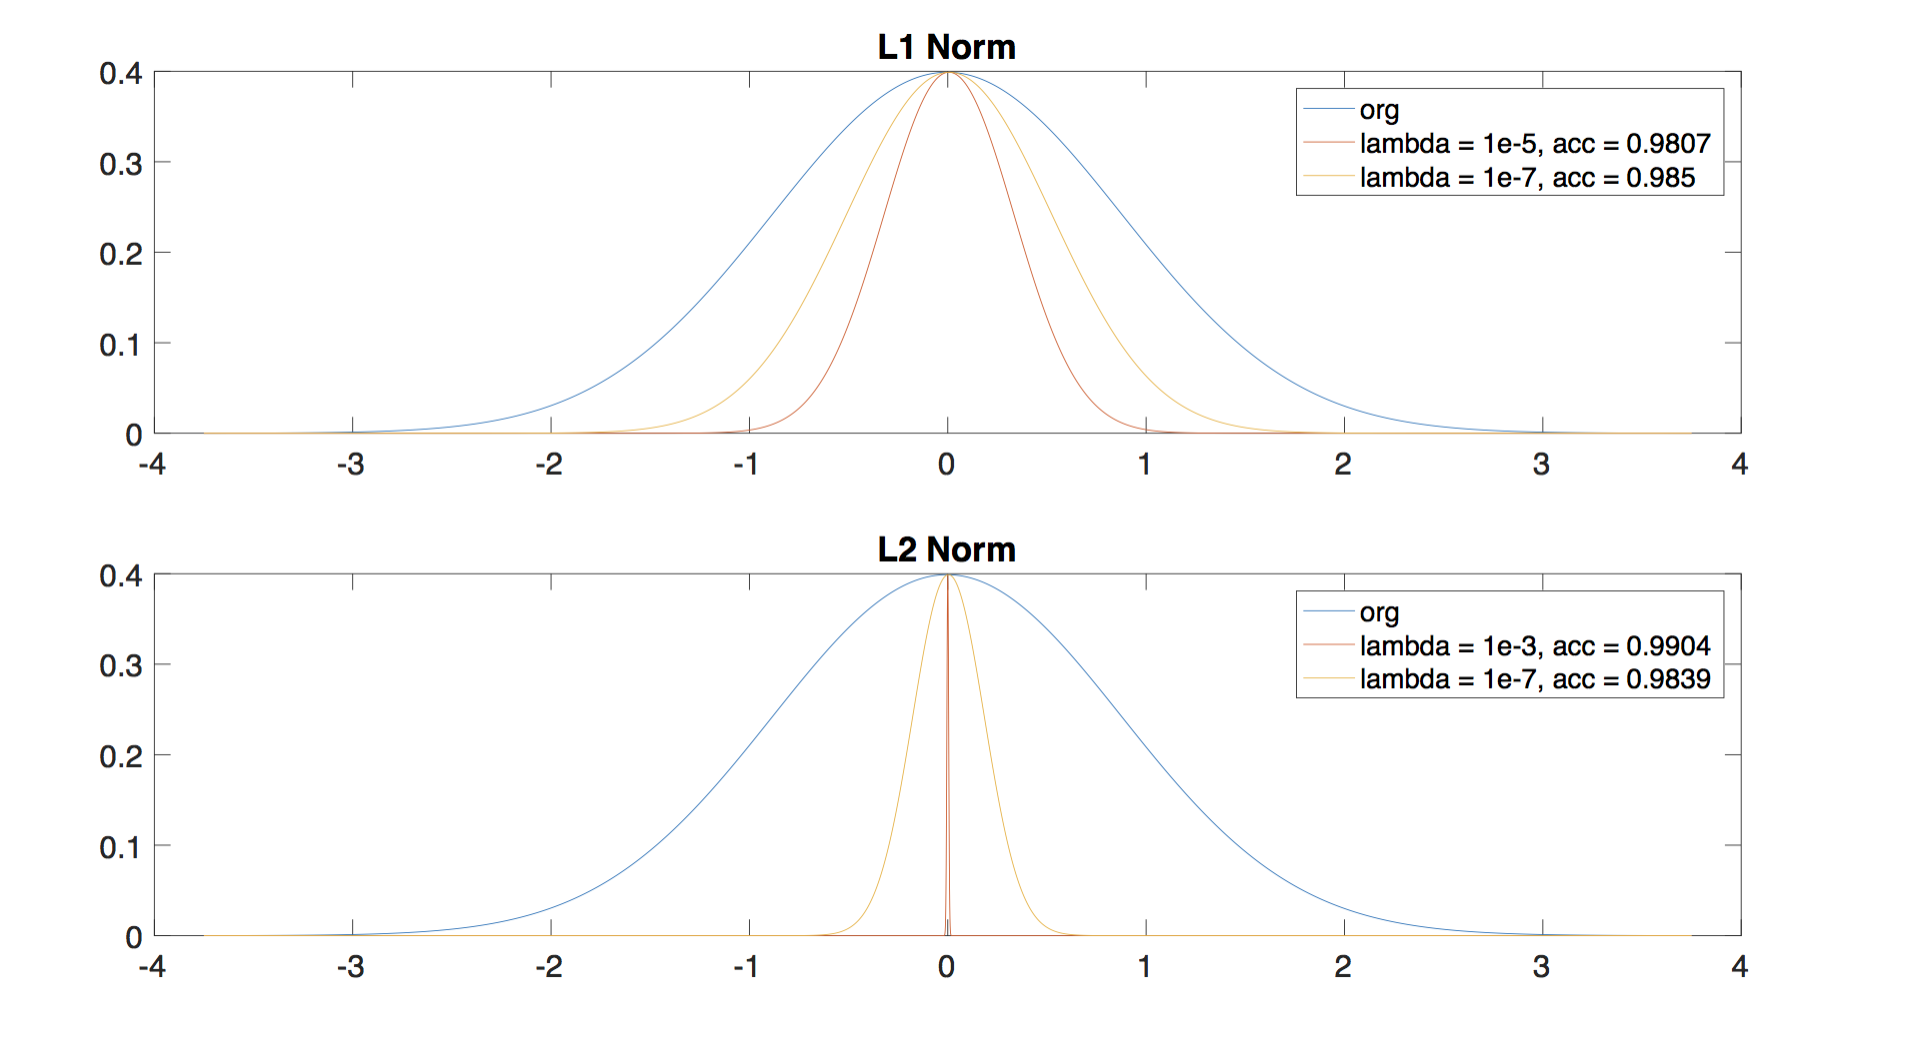
\includegraphics[width=\textwidth]{l1l2norm.png}
\caption{\label{fig:l1l2norm}Effects of $l1$ and $l2$ norms with different hyperparameters.}
\end{figure}

$\lambda{1}$ and $\lambda{2}$ are two hyperparamters that
are normally chosen arbitrarily.
To view the effect of various norms on the weights distribution of a
given neural network, \Cref{fig:l1l2norm} shows how the weights distribution
of a \textit{LeNet5} model varies when applied with different norms.
With larger $\lambda{1}$ and $\lambda{2}$ values, the weights distributions
are more concentrated to zero.

Notice in \Cref{fig:l1l2norm}, $l1$ and $l2$ norms are shown separately,
meaning that $\lambda_{2}$ and $\lambda_{1}$ in \Cref{equ:norms} are set to
zeros respectively when chosen to demonstrate the effect of $l1$ norm
and $l2$ norm respectively.
For the first plot in \Cref{fig:l1l2norm}, $l_2$ norm is set to zero and it is
obvious that when $\lambda_1$ reaches $1e^{-5}$, the weights distribution are
more concentrated at zero (red) compard to the original weights distribution (blue).
For the original distribution, both $\lambda_1$ and $\lambda_2$ are zeros.
A similar pattern is observed for the second plot in \Cref{fig:l1l2norm}: with a
larger $\lambda_2$ value, the weights distribution is more concentrated at zero.

For the hyperparameters of the regularizer, I pick $\lambda_1 = 1e^{-4}$ and $\lambda_2 = 1e^{-7}$ for \textit{LeNet5}.
The model is then pruned and retrained to an error rate of $0.64\%$.
The detailed layer-wise pruning information is shown in \Cref{tab:LeNetprunel1l2}
and compared to the best performance pruning method from the previous chapter (\textit{Dynamic network surgery}).

\begin{table}[!h]
\centering
\begin{tabular}{|l|l|l|l|l|}
\hline
Layer			&cov1	    &cov2	&fc1	&fc2 	\\	 \hline
Params		& 0.5K		&25K	&400K	&5K \\ \hline
Prune(a) \%	& 22.11\%		&92.47\%	&99.70\%	&32.91\%	\\
\hline
Prune(b) \%	& 36.54\%		&87.90\%	&99.66\%	&18.42\%	 \\
\hline
\end{tabular}
\caption{Number of parameters of pruned LeNet5-431K.
Prune(a) is \textit{Regularization aided pruning} with $l1$ and $l2$ norms,
$\lambda_1 = 1e^{-4}$ and $\lambda_2 = 1e^{-7}$.
Prune(b) is \textit{Dynamic network surgery}.}
\label{tab:LeNetprunel1l2}
\end{table}

For \textit{CifarNet}, $\lambda_{1} = 1e^{-5}$ and $\lambda_{2} = 1e^{-5}$
are selected after exploring a range of values.
The layer-wise pruning results of \textit{CifarNet} are shown
in \Cref{tab:CifarNetPrunel1l2}.
This trained \textit{CifarNet} remains a test accuracy of $0.82$, which is the
same as the original network.
\begin{table}[!h]
\centering
\begin{tabular}{|l|l|l|l|l|l|}
\hline
Layer			&cov1	&cov2		&fc1		&fc2		&fc3		\\ \hline
Params		& 4.8K		&102.4K	&885K	&74K		&2K 	\\
\hline
Prune(a) \%	& 45\%		&88\%	&96\%	&76\%	&39.6\% \\
\hline
Prune(b) \%	& 53\%		&87\%	&95\%	&82\%	&26\% \\
\hline
\end{tabular}
\caption{Number of parameters of pruned CifarNet.
Prune(a) is \textit{Regularization aided pruning} with $l1$ and $l2$ norms,
$\lambda_1 = 1e^{-5}$ and $\lambda_2 = 1e^{-5}$.
Prune(b) is \textit{Dynamic Network Surgery}.}
\label{tab:CifarNetPrunel1l2}
\end{table}

From the results in both \Cref{tab:LeNetprunel1l2}, \Cref{tab:CifarNetPrunel1l2},
\textit{Regularization aided pruning} demonstrates its performance by showing
greater compression rates on both networks.
For the \textit{LeNet5} model, the compression rate now reaches $63$x and
\textit{CifarNet} achieves a compression rate of $15.4$x.
It can be concluded that the use of regularizers encourage sparsity in the
network and thus provide better pruning results.

\section{Summary of Pruning Methods}
\label{sec:pruning_sum}
In this section, I would like to summarize all pruning methods implemented in
this project.
Some pruning methods haven been compared to their original implementations in
\Cref{sec:pruning_ext_comp}, this section only focuses on comparing my implementations
of various pruning strategies on selected datasets.



\begin{table}[!h]
  \centering
  \begin{tabular}{llllllll}
    \hline
    Model   &Layer     &Params    &(a)    &(b)      &(c)    &(d)      &(e)\\
    \hline
    \textit{LeNet5}  &cov1     &0.5K       &60\%   &48.1\%   &63.5\% &65.8\%   &78.9\%\\
            &cov2     &25K        &20\%   &20.2\%   &12.1\% &8.9\%    &7.5\%\\
            &fc1      &400K       &2\%    &0.6\%    &0.4\%  &0.7\%    &0.3\%\\
            &fc2      &5K         &60\%   &50.1\%   &82.6\% &72.2\%   &67.1\%\\
            &total    &431K       &3.8\%  &2.4\%    &2.0\%  &2.0\%    &1.6\%\\
    \hline

            &CR       &-          &26x     &42x       &49x  &48x      &63x\\
            &ER       &-          &0.64\%  &0.64\%    &0.64\% &0.64\% &0.64\%\\
    \hline
  \end{tabular}
  \caption{LeNet5 Pruning Summary, CR is the compression
  rate, ER is the error rate. (a) is \textit{Deterministic pruning} with weights and biases, (b) is
  \textit{Deterministic pruning} with weights only, (c) is \textit{Dynamic network surgery},
  (d) is \textit{Gradient profiling} and (e) is \textit{Regularization aided pruning}.}
  \label{fig:prune_new_summary}
\end{table}

\begin{table}[!h]
  \centering
  \begin{tabular}{lllllll}
    \hline
    Model   &Layer     &Params    &(a)  &(b)      &(c) &(d)  \\
    \hline
    CifarNet  &cov1     &4.8K     &70\%   &60\%   &47\% &55\%\\
            &cov2     &102.4K     &33\%   &31\%   &13\% &12\%\\
            &fc1      &885K       &15\%   &15\%   &5\% &4\%\\
            &fc2      &74K        &33\%   &31\%   &18\% &24\%\\
            &fc3      &2K         &70\%   &60\%   &74\% &60\%\\
            &total    &1068K      &18.5\%  &17.9\%  &7.0\% &6.5\%\\
    \hline

            &CR       &-          &5.41x   &5.58x  &14.3x   &15.4x\\
            &ER       &-          &18\%   &18\%  &18\%   &18\%\\
    \hline
  \end{tabular}
  \caption{\textit{CifarNet} Pruning Summary, CR is the compression
  rate, ER is the error rate. (a) is \textit{Deterministic pruning} with weights and biases, (b) is
  \textit{Deterministic pruning} with weights only, (c) is \textit{Dynamic network surgery}
  and (d) is \textit{Regularization aided pruning}.}
  \label{fig:cifar_prune_new_summary}
\end{table}
Similar to the previous setup, \Cref{fig:prune_new_summary} shows the pruning
results.
The percentiles showing for each layer represents the amount of
parameters left in that layer.
To prune \textit{LeNet5}, it is important to achieve a small percentage on
the first fully-connected layer (fc1), since it contains a large number of
parameters.
Method (a) is \textit{Deterministic pruning} with weights and biases, (b) is
\textit{Deterministic pruning} with weights only, (c) is \textit{Dynamic network surgery},
(d) is \textit{Gradient profiling} and (e) is
\textit{Regularization aided pruning}.
The proposed pruning strategy, \textit{Regularization aided pruning}, achieves
the best compression rate: it shows a $1.3$x increase in compression rate compared
to \textit{Dynamic network surgery} on the \textit{LeNet5} model.

Similarly, the pruning summary of \textit{CifarNet} demonstrated that
\textit{Regularization aided pruning} achieves the best compression result.
The compression rate now reaches $15.4$x without any loss of test accuracies.
The following important observations can be summarized from comparing a range
of pruning methods:
\begin{enumerate}
  \item Pruning with only weights is more efficient.
  \item Non-deterministic pruning achieves better compression rates since pruned weights now have chance to recover.
  \item Gradients can serve as indications for identifying important weights.
  \item The use of regularizers helps pruning by encouraging sparsity in the network,
  and thus \textit{Regularization aided pruning} shows the best pruning results.
\end{enumerate}

\chapter{Quantization}
The objective of this chapter is to discover an efficient number representation
system.
An efficient number representation system reduces the number of bits
required to represent individual parameters, and thus offers a compression
on the top of pruning.
In this section, I aim to investigate various existing quantization methodologies to further
compress the chosen neural networks.
Traditionally, a neural network is trained on GPUs in 32-bit floating-point
representation, however, this representation becomes problematic on low power devices.
First, using 32 bits to store a single parameter is proven to be redundant
\cite{mellempudi2017mixed}.
Second, floating-point arithmetic operations are generally more power-consuming than
fixed-point operations.
Methods such as \textit{Weights sharing} are discussed in this section
\cite{Han15}.
Low-precision arithmetics, including \textit{Fixed-point arithmetic} and \textit{Dynamic fixed-point
arithmetic}, are also compared and evaluated.

\section{Weights Sharing}
\textit{Weights sharing} compresses the bit-width of parameters using a codebook and stores only
the indexes.
Similar to \textit{HashNet} \cite{chen2015compressing}, \textit{Weights sharing} used in \textit{Deep Compression}
\cite{Han15} can reduce the number of bits required
to represent a parameter by employing a hash function and store weights as hash keys (indexes).
Designing the hash function firstly requires grouping of weights.
In this case, following the implementation of \textit{Han et al.} \cite{Han15},
I performed \textit{K-means} clustering \cite{kanungo2002efficient}
to group weights into $n$ clusters, and therefore $n$ centroid values are produced.

The inference and retraining of grouped weights are illustrated in
\Cref{fig:weights_share}.
Consider a small four-by-four weight matrix, and weights are grouped into $4$ groups.
Only the cluster indexes and codebook (effective weights) need to be stored for network inference.
For this particular example, to represent $4$ clusters, each weight can
be represented using only a 2-bit cluster index.
The use of index and codebook directly compressed the size of a neural network, and \textit{Han et al.}
have summarized an equation for the compression rate \cite{Han15}.
Given $k$ clusters, $\log_{2}(k)$ bits are required for encoding the index.
Consider a neural network with $N$ parameters, and each parameter is $b$ bits
wide, the following equation summarizes the compression rate $CR$:
\begin{equation}
CR = \frac{Nb}{N\log_2(k) + kb}
\label{equ:weightsshare_cr}
\end{equation}


\begin{figure}[!h]
\centering
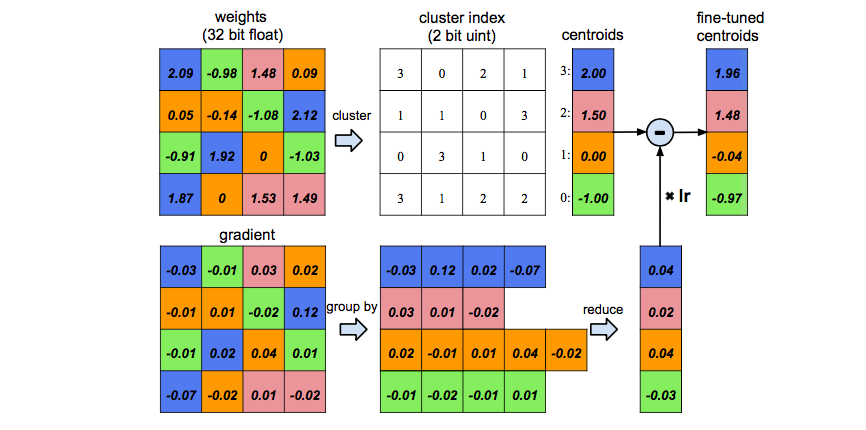
\includegraphics[width=\textwidth]{fig_weights_share.png}
\caption{\label{fig:weights_share}Weights sharing: training (bottom) and inference (top) \cite{Han15}.}
\end{figure}

This \textit{Weights sharing} technique is applied on both \textit{LeNet5} and
\textit{CifarNet}.
\Cref{tab:ws_sum} shows the quantization results of \textit{Weights sharing} on
the targeting neural networks.
\textit{Weights sharing} is also combined with retraining to bring back the
lost test accuracies.
\Cref{tab:ws_sum} uses two rows for each neural network, one row represents the test accuracies
before retraining and one row shows the accuracies after retraining.
First, as expected, test accuracies are significantly larger when the number of clusters
is large.
Second, retraining is demonstrated to be an efficient method of brining back the
lost accuracies.
\textit{Weights sharing} worked very well on \textit{LeNet5}, with 8 clusters at each
layer, \textit{LeNet5} achieves no accuracy loss after retraining.
It is important to note that, for 8 clusters, only 3 bits are required to
represent the cluster index of each parameter.

\begin{table}[!h]
  \centering
  \begin{tabular}{lllllll}
    \hline
    \hline
    Number of clusters      &64         &32       &16       &8        &4        &2  \\
    \hline
    Number of bits          &6         &5       &4       &3        &2        &1  \\
    \hline
    \hline
    \multicolumn{5}{l}{\textbf{\textit{LeNet5}}, 32-bit floating point accuracy: 99.36\%}\\
    \hline
    Before Retrain          &99.36\%    &99.36\%  &99.36\%  &99.29\%  &98.90\%  &94.67\%\\
    After Retrain           &99.36\%    &99.36\%  &99.36\%  &99.36\%  &99.15\%  &98.66\%\\
    \hline
    \hline
    \multicolumn{5}{l}{\textbf{\textit{CifarNet}}, 32-bit floating point accuracy: 82.00\%}\\
    \hline
    Before Retrain          &79.94\%    &79.81\%  &72.78\%  &69.00\%  &25.25\%  &9.94\%\\
    After Retrain           &82.21\%    &82.01\%  &82.02\%  &79.05\%  &65.70\%  &17.2\%\\
    \hline
    \hline
  \end{tabular}
  \caption{\textit{Weights sharing} summary for \textit{LeNet5} and \textit{CifarNet}.}
  \label{tab:ws_sum}
\end{table}

\textit{CifarNet} is a larger network compared to \textit{LeNet5}.
As a result of its larger size, the network requires a larger number of clusters
at each layer.
According to \Cref{tab:ws_sum}, at a cluster count of 16,
the network achieves no accuracy loss.
This means, each weight parameter can be represented using 4 bits, and
the neural network is able to achieve the same accuracy as the uncompressed
one.
% \begin{figure}[!h]
%   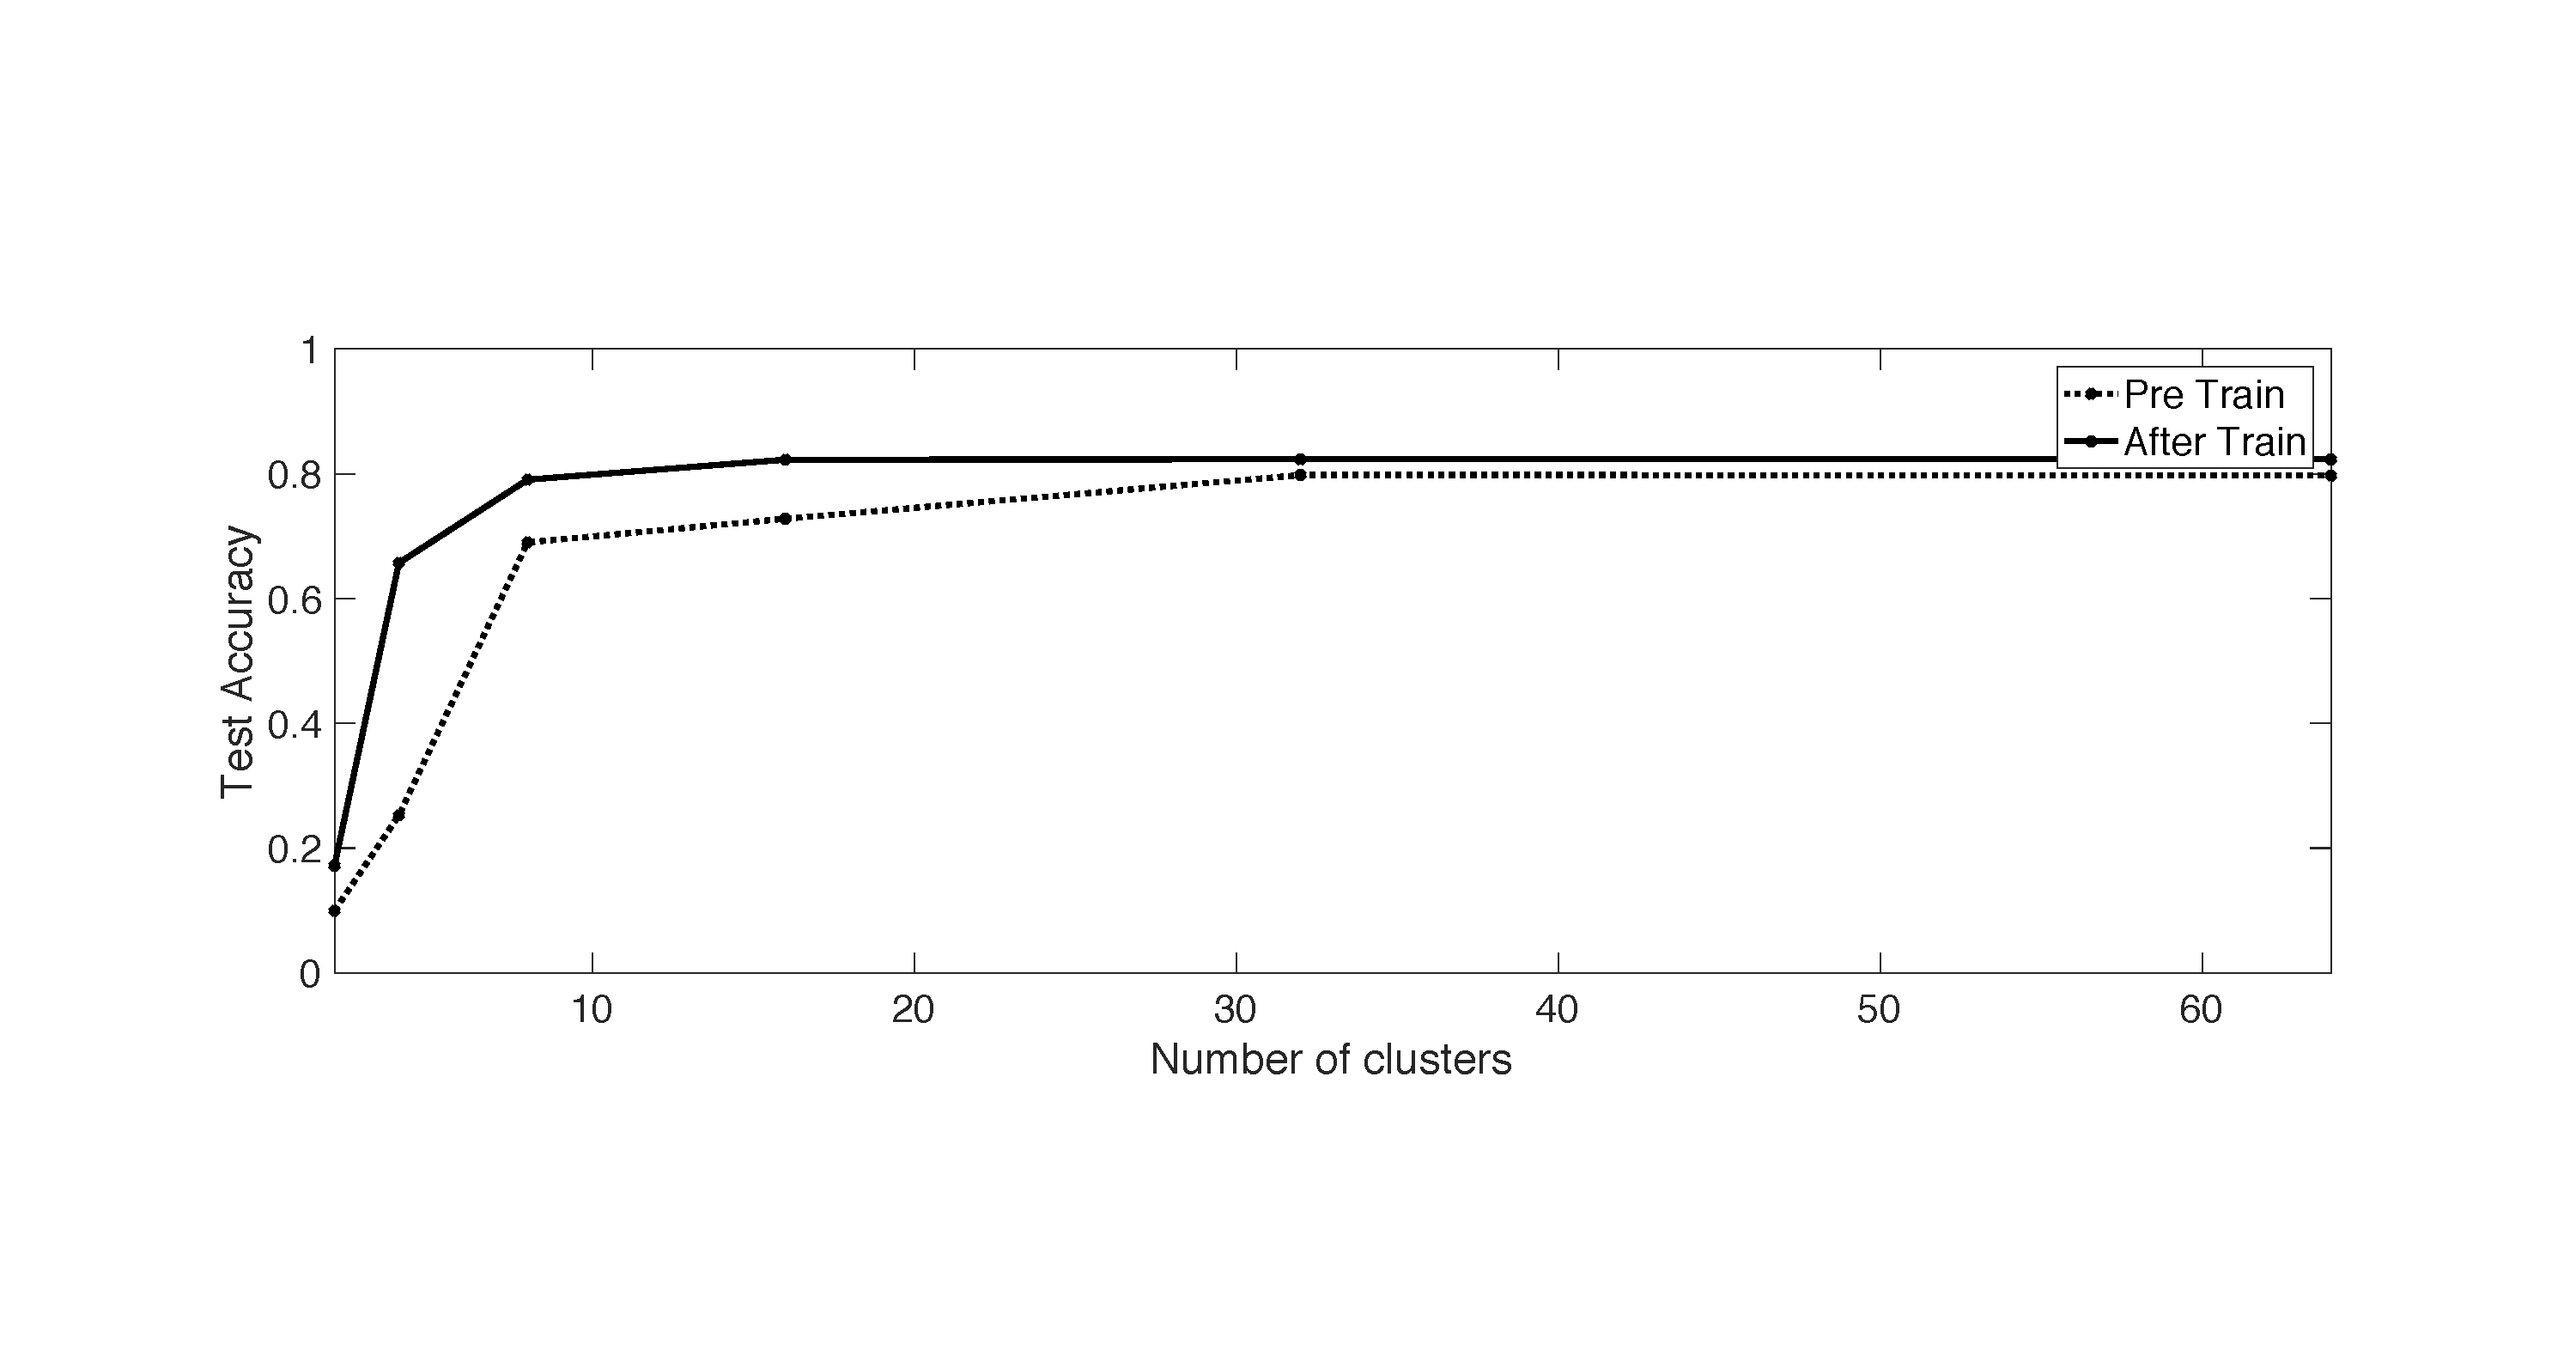
\includegraphics[width=\textwidth]{Cifar10_han.pdf}
%   \caption{Test accuracies for clustered weights in CifarNet.}
%   \label{fig:CifarNetHan}
% \end{figure}

Although \textit{Weights sharing} demonstrated good compression rates on both networks,
the arithmetic operations are still in floating-point.
Since floating-point arithmetic operations are power consuming, turning
into small fixed-point numbers can reduce both energy consumption and circuitry
area.
In \textit{Han et al.'s} imeplementation, they used \textit{Weights sharing}
on top of \textit{Fixed-point quantization}.
In later sections, the focus stays on exploring fixed-point based quantization
methods.

\section{Fixed-point Quantization}
One simple quantization strategy when using fixed-point arithmetic is to truncate
the least significant bits (LSBs) but leave the most significant bits (MSBs)
unchanged.
This method is straightforward and easy to implement.
\begin{figure}[!h]
\centering
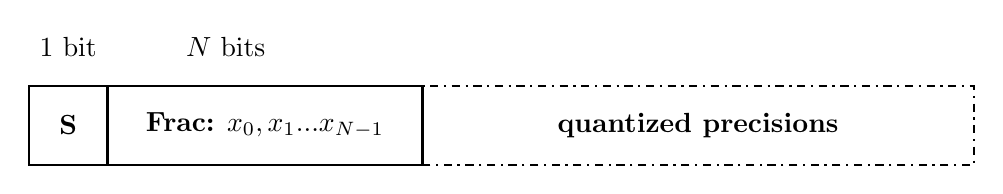
\begin{tikzpicture}
  \draw[style=thick] (0,0) rectangle (1,1) node(sign)[pos=.5] {\textbf{S}};
  \draw[style=thick] (1,0) rectangle (5,1) node(frac)[pos=.5] {\textbf{Frac:} $x_0, x_1 ... x_{N-1}$};
  \draw[thick,dash dot] (5,0) rectangle (12,1) node(ignored)[pos=.5] {\textbf{quantized precisions}};
  \node[] at (.5,1.5) {$1$ bit};
  \node[] at (2.5,1.5) {$N$ bits};
\end{tikzpicture}
\caption{Number representation system for fixed-point quantization with 1-bit
sign and N-bit fraction.}
\label{fig:number_rep_4bit}
\end{figure}

\Cref{fig:number_rep_4bit} shows the number representations of a quantized number.
The number representation system has $1$ bit for sign and
$N$ bits for fractions.
The number of fractional bits can be therefore changed to track numbers to various
levels of precisions.
\Cref{equ:d2fp} shows how the number representation of \Cref{fig:number_rep_4bit}
can be converted to decimal representation.
In this case, $S$ stands for the sign bit, $N$ is the total number
of fractional bits.
$x_i$ represents the fractional bit values.
The representation used in this section is a traditional signed fixed-point
representation with $N$-bit fractions \cite{ercegovac2004digital}.

\begin{equation}
    D = (-1)^S (\sum^{N-1}_{i=0}2^{-i}x_i)
    % \caption{Decimal to fixed-point conversion}
    \label{equ:d2fp}
\end{equation}

\Cref{tab:fp_sum} shows how fixed-point quantization performs on \textit{LeNet5}
and \textit{CifarNet} when the bit-width changes.
It is important to note that, the bit-width in this case refers to total bit-width.
Total bit-width is $N+1$, including $N$-bit fractions and $1$-bit sign.

\begin{table}[!h]
  \centering
  \begin{tabular}{llllll}
    \hline
    \hline
    Bit width               &32-bit     &16-bit     &8-bit    &4-bit    &2-bit  \\
    \hline
    \multicolumn{5}{l}{\textbf{\textit{LeNet5}}, 32-bit floating point accuracy: 99.36\%}\\
    \hline
    \hline
    Before Retrain          &98.98\%    &97.08\%    &75.63\%    &12.74\%  &9.78\%\\
    After Retrain           &99.36\%    &99.36\%    &99.26\%    &98.88\%  &9.78\%\\
    \hline
    \hline
    \multicolumn{5}{l}{\textbf{\textit{CifarNet}}, 32-bit floating point accuracy: 82.00\%}\\
    \hline
    Before Retrain          &32.84\%        &21.58\%    &12.16\%  &10.22\%  &9.97\%\\
    After Retrain           &82.00\%        &79.21\%    &68.76\%  &65.76\%  &9.95\%\\
    \hline
    \hline
  \end{tabular}
  \caption{Fixed-point quantization summary for \textit{LeNet5} and \textit{CifarNet}.}
  \label{tab:fp_sum}
\end{table}

The results in \Cref{tab:fp_sum} suggests that 16 bits for \textit{LeNet5}
achieves best quantization results without any accuracy loss.
32-bit is redundant since the test accuracy remains the same as 16-bit when
retraining is applied.
Similar to the previous setup, retraining occurs after quantization to bring
back test accuracies.
Retraining takes a very important role in fixed-point quantization.
For instance, when $LeNet5$ is quantized to 4-bit (3-bit fraction and 1-bit sign),
its test accuracy before retraining is only $12.74\%$, but increases to $98.88\%$ after retraining.
As illustrated in \Cref{tab:fp_sum}, \textit{CifarNet} only recovers to an accuracy
of $79.21\%$ when the precision is 16-bit and $82.00\%$ when the precision is
32-bit.
Since \textit{CifarNet} is a larger neural network compared to \textit{LeNet5},
it requires more bits to retain its test accuracy.
To conclude, for \textit{fixed-point quantization}, \textit{LeNet5} is able to
use $8$ bits to represent the original neural network and 32 bits are needed for
\textit{CifarNet} to retain its test accuracies.

% \begin{figure}[!h]
% \centering
%   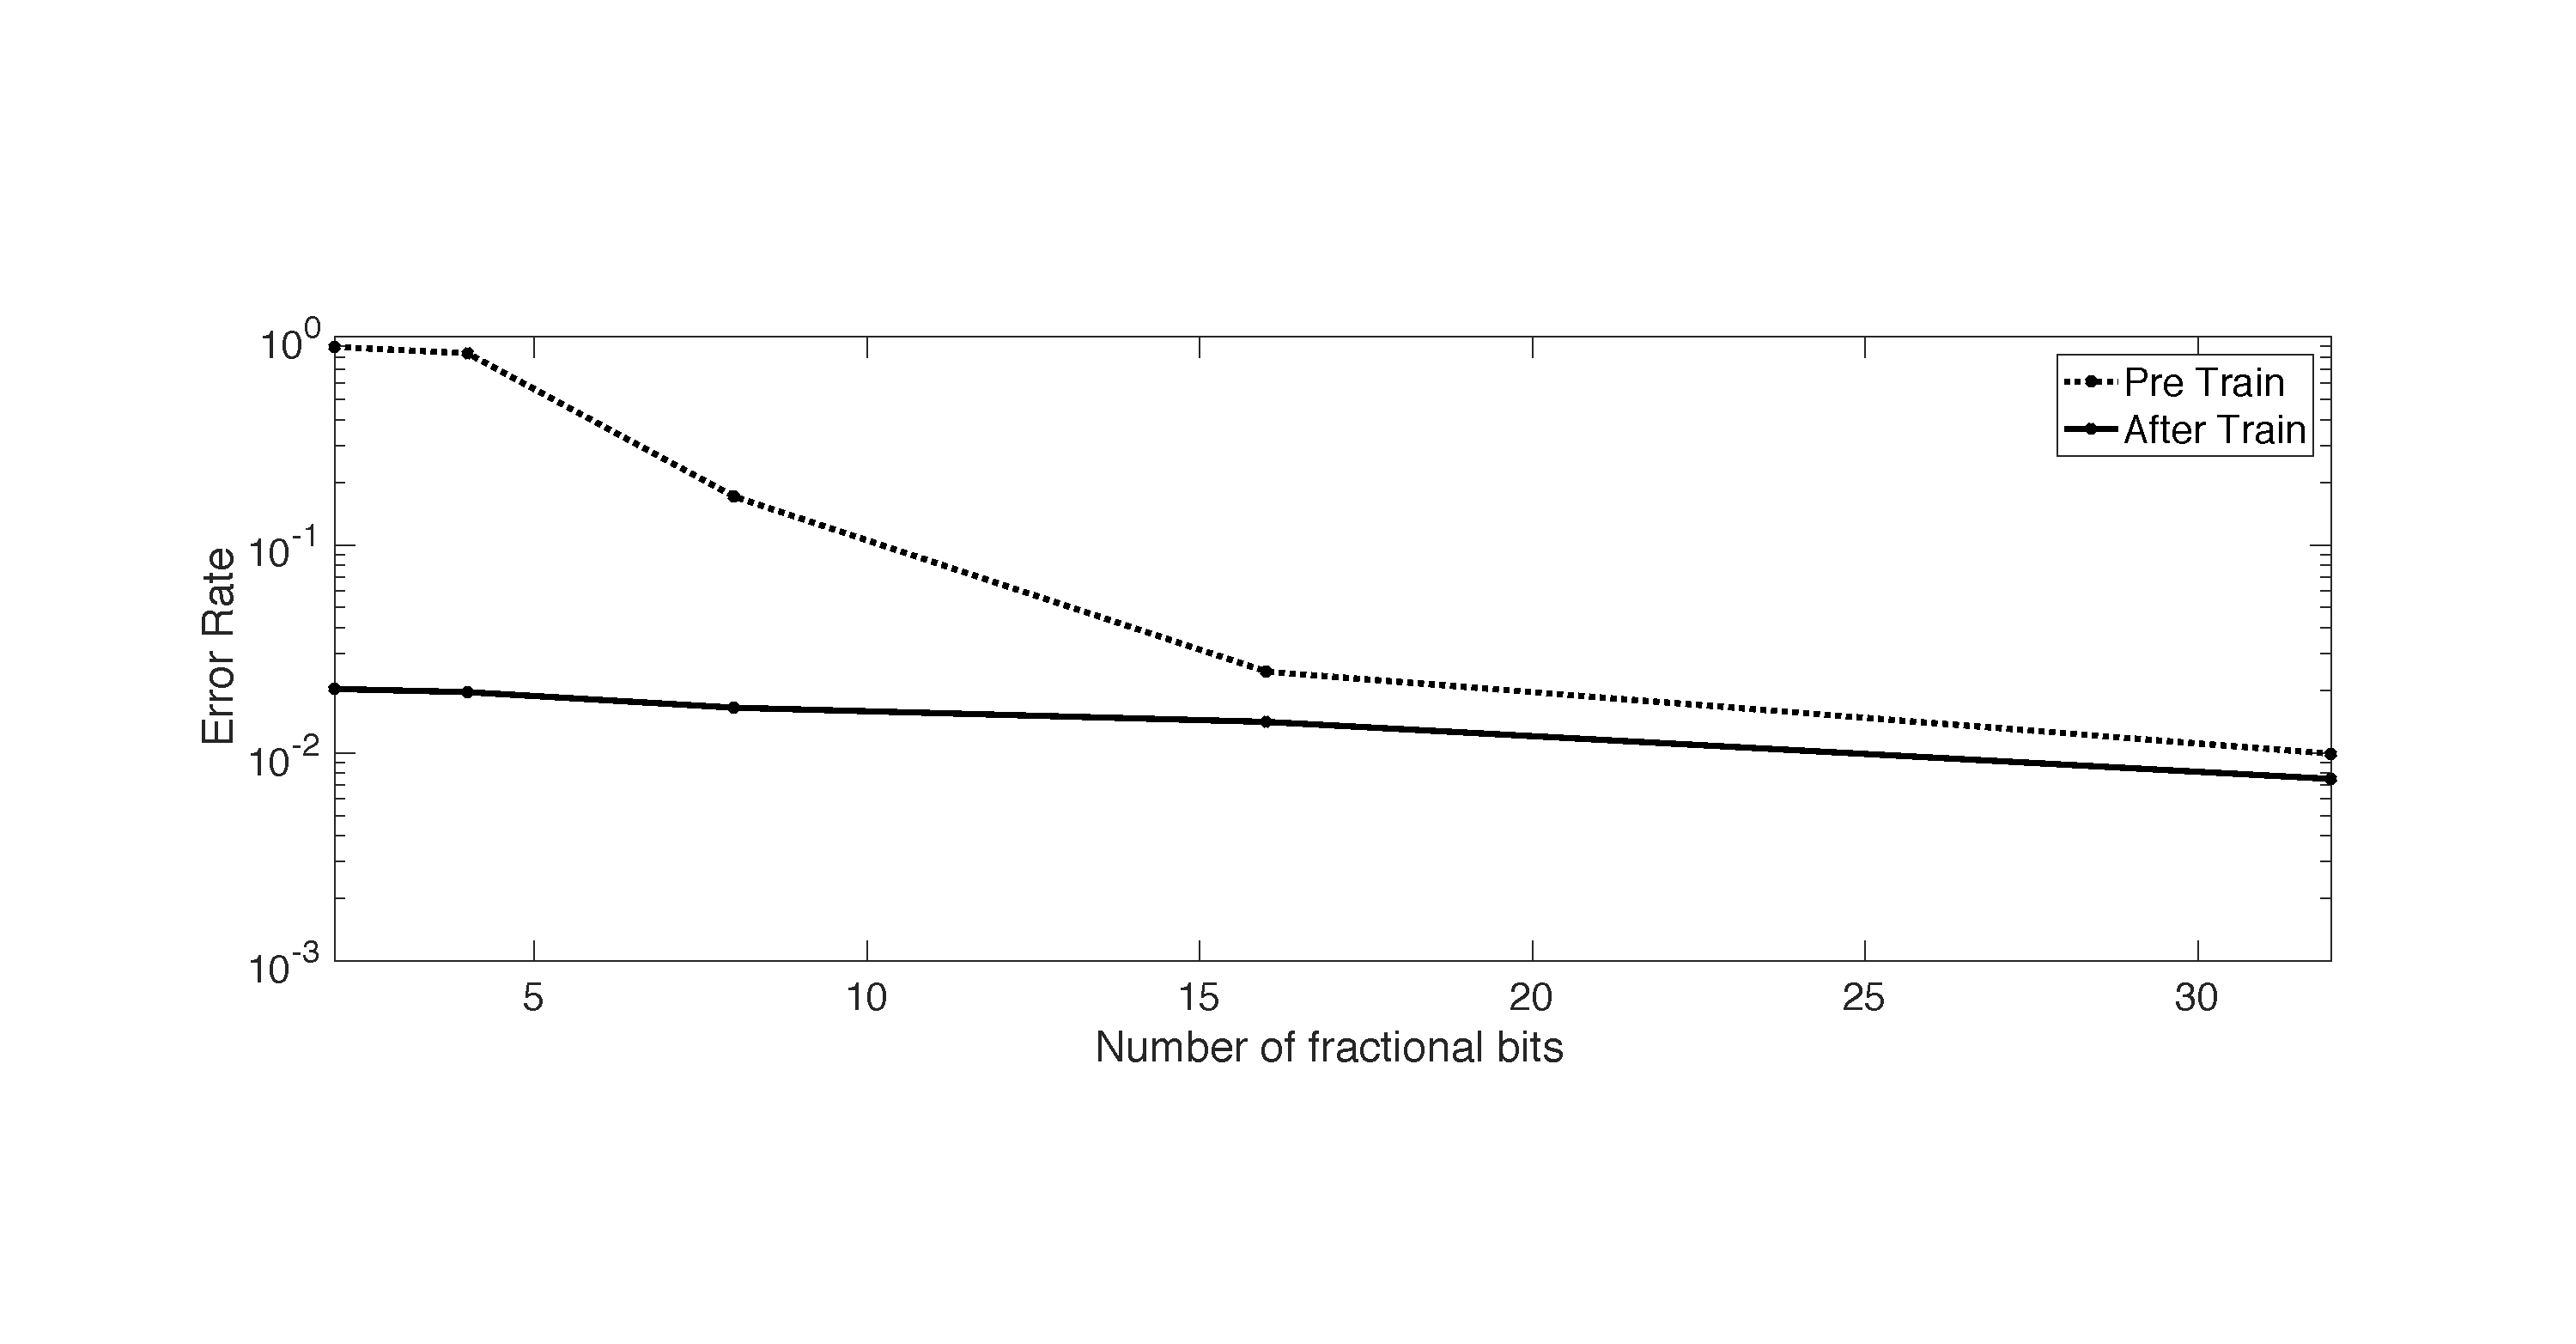
\includegraphics[width=\textwidth]{LeNet5_fp.pdf}%
%   \caption{Error rates for LetNet5 using fixed-point quantization.}
%   \label{fig:LeNetfp}
% \end{figure}
% \begin{figure}[!h]
% \centering
%   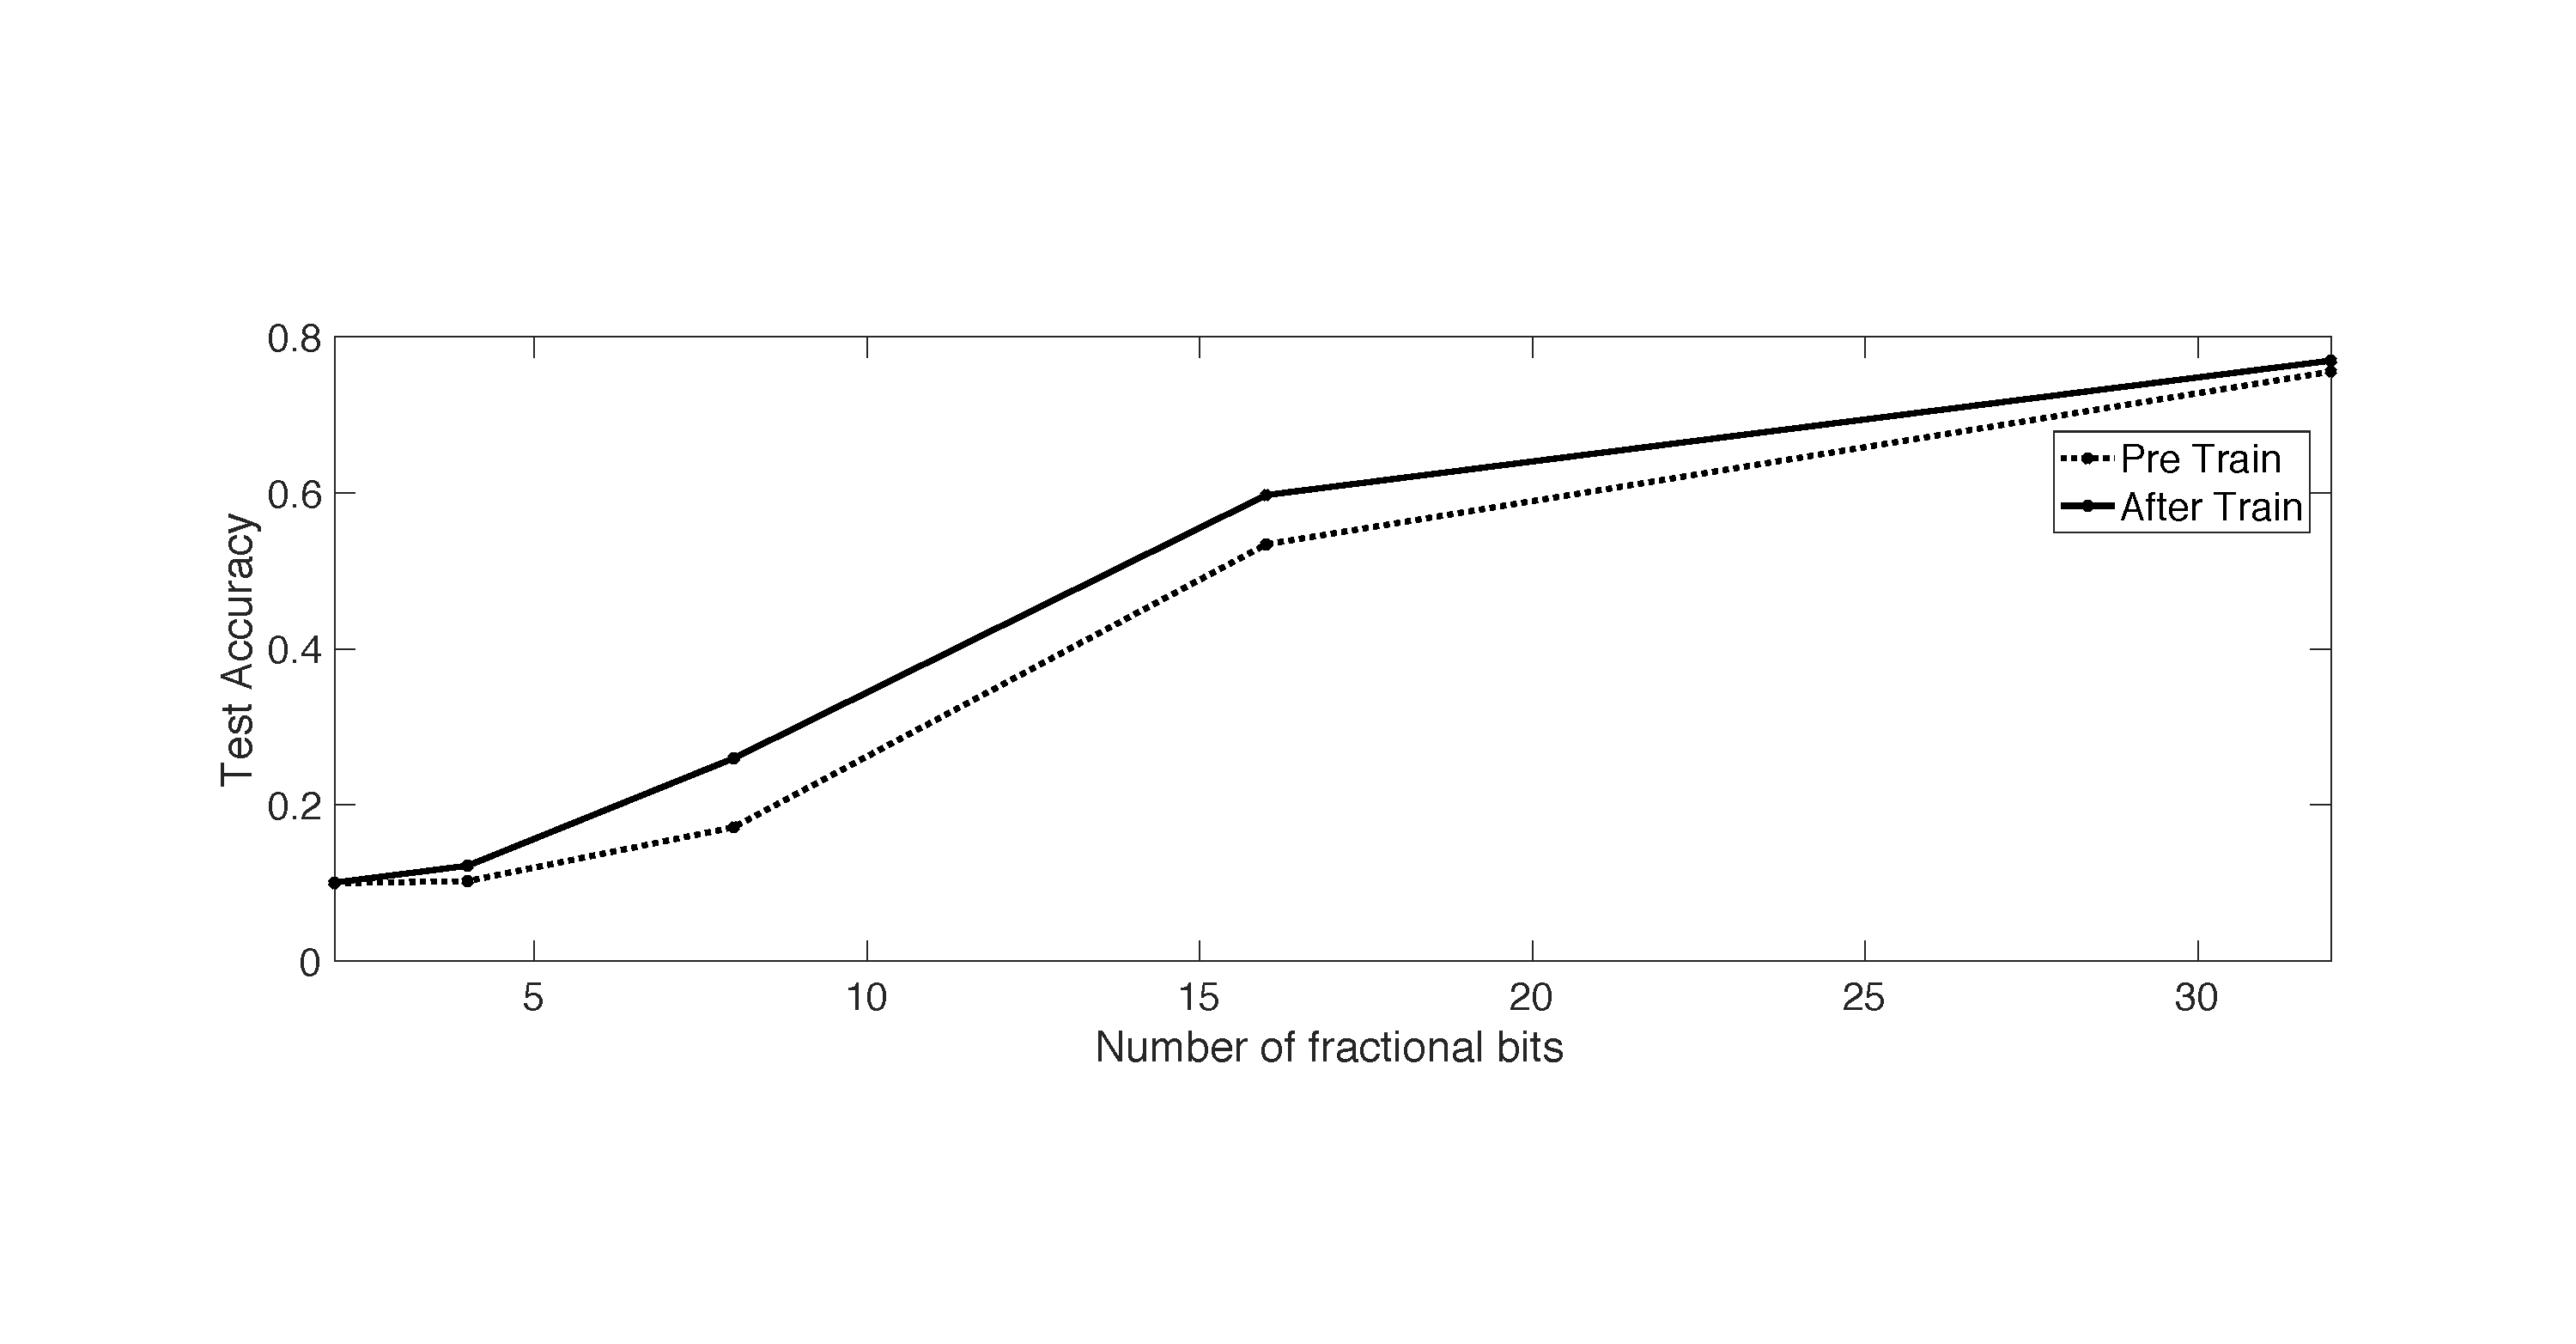
\includegraphics[width=\textwidth]{CifarNet_fp.pdf}%
%   \caption{Test accuracies for CifarNet using fixed-point quantization.}
%   \label{fig:LeNetfp}
% \end{figure}
\section{Dynamic Fixed-point Quantization}
\label{sec:dfq}
\textit{Dynamic fixed-point} arithmetic is a variant of fixed-point arithmetic,
where a number of parameters are grouped with a fixed scaling factor \cite{williamson1991dynamically}.
Previously, \textit{Courbariaux et al.} has implemented both \textit{LeNet5} and
\textit{CifarNet} using \textit{Dynamic fixed-point} arithmetic \cite{courbariaux2014training}.
They proposed an algorithm (\Cref{alg:scaling_factor}) for computing the scaling factors.
The scaling factors define the dynamic range for a selected group of weights.

To use \textit{Dynamic fixed-point} in a neural network, \Cref{alg:scaling_factor}
is applied  on each layer of parameters to help weights with various dynamic ranges.
\Cref{alg:scaling_factor} works by setting an arbitrarily defined overflow rate,
in this project, the overflow rate is set to be $10^{-3}$.
It then inspect the weights matrix and converges to a scaling factor after a
few iterations.
It is possible for weights in convolutional layers to have a completely different
dynamic range from weights in fully connected layers.
The number representation system is the same as \textit{fixed-point} arithmetic
shown in \Cref{fig:number_rep_4bit}.
The major difference now is each group of weights has a fixed dynamic range.
In \Cref{equ:d2ddfp}, it shows how a \textit{Dynamic fixed-point} number can be
converted to a decimal value.
$DR$ represents the fixed dynamic range, consider the scaling factor ($s_t$)
computed in \Cref{equ:d2ddfp}, the following relation holds: $s_t = 2^{DR}$.
These dynamic ranges, or can be viewed as scaling factors, are stored globally
for each layer and thus saves the bit-width for the number representation system.

\begin{equation}
    D = (-1)^S 2^{DR}(\sum^{M-1}_{i=0}2^{-i}xm_i)
    % \caption{Decimal to fixed-point conversion}
    \label{equ:d2ddfp}
\end{equation}

\begin{algorithm}
\caption{Scaling Factor Update} \label{alg:scaling_factor}
\begin{algorithmic}[1]
\STATE \textbf{Initialize}: matrix \textit{M}, scaling factor $s_t$ and maximum overflow rate $r_{max}$
\WHILE{$s_{t}$ doe not converge}
\IF {the overflow rate of $M > r_{max}$}
  \STATE $s_{t+1} \gets 2s_t$
\ELSIF {the overflow rate of $2M \leq r_{max}$}
  \STATE $s_{t+1} \gets s_t/2$
\ELSE
  \STATE $s_{t+1} \gets s_t$
\ENDIF
\ENDWHILE
\end{algorithmic}
\end{algorithm}

\textit{Dynamic Fixed-point} quantization has been applied on both $LeNet5$
and $CifarNet$, the results are shown in \Cref{tab:dfp_sum}.
For each bit-width count, it includes the sign bit but excludes the dynamic range.
If a bit-width of $4$ is given, this means it has $1$ bit for sign, $3$ bits for
fractions and a dynamic range that is globally defined for a given layer.
Bit-width refers to the number of total bits required to represent a number using
\textit{Dynmaic fixed-point} arithmetic, and the dynamic range is stored as a layer-wise global
value.
As expected, \textit{LeNet5} reaches the original test accuracy at a bit-width of
$4$, and \textit{CifarNet} achieves no accuracy loss after retrain at a bit-width
of $8$.
These results agree with the experimental results achieved by \textit{Courbariaux et al.}
\cite{courbariaux2014training} and \textit{Gysel et al.} \cite{Gysel}.
However, the test accuracy of retrained \textit{LeNet5} never reaches its
original test accuracy ($99.36\%$).
This indicates that \textit{Dynamic fixed-point} hurts test accuracy in a way
that even retraining cannot bring back the lost test accuracies.
In both \textit{Courbariaux et al.} and \textit{Gysel et al.}'s work, they used
a $LeNet5$ with an original test accuracy of $99.17\%$ \cite{courbariaux2014training,Gysel},
so they did not observe this effect.
Because of the high original test accuracy, my implementation of \textit{LeNet5}
is more sensitive to test accuracy deterioration.

\begin{table}[!h]
  \centering
  \begin{tabular}{llllll}
    \hline
    \hline
    Bit width               &32-bit     &16-bit     &8-bit    &4-bit    &2-bit  \\
    \hline
    \multicolumn{5}{l}{\textbf{\textit{LeNet5}}, 32-bit floating point accuracy: 99.36\%}\\
    \hline
    \hline
    Before Retrain          &88.40\%    &88.32\%    &86.92\%    &79.10\%  &71.26\%\\
    After Retrain           &99.29\%    &99.30\%    &99.31\%    &99.31\%  &99.00\%\\
    \hline
    \hline
    \multicolumn{5}{l}{\textbf{\textit{CifarNet}}, 32-bit floating point accuracy: 82.00\%}\\
    \hline
    Before Retrain          &58.99\%        &26.25\%    &10.48\%  &9.98\%  &9.98\%\\
    After Retrain           &82.00\%        &82.12\%    &82.03\%  &72.18\%  &30.53\%\\
    \hline
    \hline
  \end{tabular}
  \caption{\textit{Dynamic fixed-point quantization} summary for \textit{LeNet5} and \textit{CifarNet}.}
  \label{tab:dfp_sum}
\end{table}

By observing the dynamic range of fixed-point quantization, I can practically
find the reason for this loss of accuracy caused by using \textit{Dynamic fixed-point}.
Consider the scaling factor determined using \Cref{alg:scaling_factor}, this
scaling factor restricts the range of values that this arithmetic could represent.
For instance, a scaling factor of $0.5$ is determined for the first fully
connected layer by inspecting the pre-quantized \textit{LeNet5} model.
However, for a $LeNet5$ model that is quantized using fixed-point arithmetic and
achieved no accuracy loss, its maximum value in that layer reaches $0.406$ but
minimum value reaches $-0.55$.
In this case, if \textit{Dynamic fixed-point} is applied with a scaling factor of $0.5$, values that are lower
than $-0.5$ will never be reached.
The hypothesis is that the loss of dynamic range can potentially affect retraining
since now the quantized weights is restricted to certain numerical ranges.
This hypothesis is not theoretically proven, but is hinted by comparing both
the test accuracies and numerical ranges of \textit{Fixed-point} arithmetic
and \textit{Dynamic fixed-point} arithmetic.
A theoretical proof of this hypothesis is beyond the scope of this project, but
could be evaluated in future works.

For the experimental results shown in \Cref{tab:dfp_sum}, \textit{LeNet5} is
able to represent the parameters using $4$ bits and achieve a test accuracy of
$99.31\%$.
Although it suffers from a slight test accuracy drop, it offers a much better
quantization result.
For \textit{CifarNet}, it is able to quantize to a bit-width of $8$ with no loss
of test accuracies.

\chapter{Optimized Quantization Strategies}
In the previous chapter, a number of existing quantization methods have been
implemented and evaluated.
In this chapter, I would like to propose some new quantization methods for
compressing neural networks.
First, a \textit{Customized floating-point} arithmetic is proposed and it overcomes
certain limitations of \textit{Dynamic fixed-point} arithmetic and also showed
better performance compared to \textit{Dynamic fixed-point}.
Second, to quantize a pruned model, I applied some bi-centralized arithmetics
to fully explore the weights distribution by re-centralizing the precision
centres of arithmetics.

\section{Customized Floating-point Quantization}
In this section, I propose a new number representation system that stands in
the middle between \textit{Dynamic fixed-point} arithmetic and
\textit{Floating-point} arithmetic.

In \textit{Dynamic fixed-point}, each number is represented as:
$(-1)^S2^{-\textit{DR}}\sum^{M-1}_{i=0}2^ix_i$.
$M$ denotes the mantissa width, $S$ is the sign bit, $\textit{DR}$ is the dynamic range
and $x$ are the mantissa bits \cite{courbariaux2014training, Gysel}.
At various layers of the neural network, \textit{Dynamic fixed-point} assigns
fixed-point numbers with different layer-wise dynamic ranges ($\textit{DR}$).
This $\textit{DR}$ value stays unchanged for the grouped weights in one layer.
In contrast, \textit{Floating-point arithmetic} has a changing exponent for each
individual weight, and therefore the decimal point is floating.
A normal floating-point number can be expressed as $(-1)^S2^{\textit{exp}-\textit{offset}}\sum^{M-1}_{i=0}2^ix_i$.
In this case, an \textit{offset} value is included to help the arithmetic to cover a large
range of values \cite{ercegovac2004digital}.
\begin{figure}[!h]
\centering
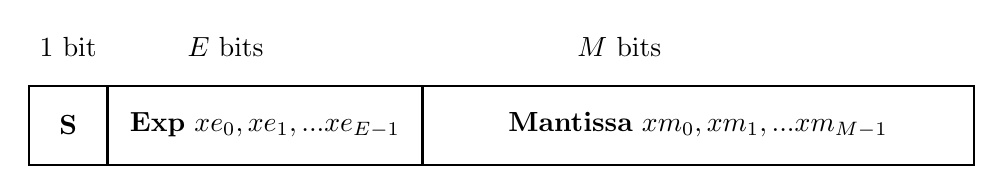
\begin{tikzpicture}
  \draw[style=thick] (0,0) rectangle (1,1) node(sign)[pos=.5] {\textbf{S}};
  \draw[style=thick] (1,0) rectangle (5,1) node(frac)[pos=.5] {\textbf{Exp} $xe_0, xe_1, ... xe_{E-1}$};
  \draw[thick] (5,0) rectangle (12,1) node(ignored)[pos=.5] {\textbf{Mantissa} $xm_0, xm_1, ... xm_{M-1}$};
  \node[] at (.5,1.5) {$1$ bit};
  \node[] at (2.5,1.5) {$E$ bits};
  \node[] at (7.5,1.5) {$M$ bits};
\end{tikzpicture}
\caption{Number representation system for customized floating-point quantization with
e-bit exponent and m-bit mantissa.}
\label{number_rep_dfp}
\end{figure}

Different from both arithmetics, \textit{Customized floating-point} arithmetic only
needs to track values smaller than $1$, so the \textit{offset} value in normal floating-point
is eliminated.
Consider the number representation system in \Cref{number_rep_dfp}, the following
equation summarizes its conversion to a decimal value:

\begin{equation} \label{equ:d2dfp2}
    D = (-1)^S 2^{-\sum^{E-1}_{i=0}2^{-i}xe_i}(\sum^{M-1}_{i=0}2^{-i}xm_i)
    % \caption{Decimal to fixed-point conversion}
\end{equation}

In \Cref{equ:d2dfp2}, $D$ represents expected decimal value, $S$ is the sign
bit, $M$ is the mantissa width and $E$ is the exponent width.
$xm_i$ are the mantissa bits and $xe_i$ are the exponent bits.

As shown in \Cref{equ:d2dfp2}, each individual weight now takes its own
dynamic range, so this is different from \textit{Dynamic fixed-point} where
only a fixed dynamic range is allowed for a group of parameters.
More importantly, the dynamic range now is restricted to be lower than $1$,
this makes sure the arithmetic tracks to lowest possible precisions given
a limited bit-width.

\Cref{tab:cfp_sum} shows the quantization results.
Using only 6 bits, \textit{Customized floating-point} is able to generate a retrained
\textit{LeNet5} that has no accuracy loss.
For \textit{CifarNet}, a bit-width of $8$ is required for it to recover
to the original accuracy.
In \Cref{tab:cfp_sum}, the bit-width includes both a sign bit and a 2-bit exponent.
The exponent is chosen to be $2$ bits for both \textit{LeNet5} and \textit{CifarNet}.
For instance, given a bit width of $6$ bits, it consumes $1$ bit for sign, $2$
bits for exponent and only $3$ bits are left for mantissa.

\begin{table}[!h]
  \centering
  \begin{tabular}{llllll}
    \hline
    \hline
    Bit width               &32-bit     &16-bit     &8-bit     &6-bit      &4-bit    \\
    \hline
    \multicolumn{5}{l}{\textbf{\textit{LeNet5}}, 32-bit floating point accuracy: 99.36\%}\\
    \hline
    \hline
    Before Retrain          &99.36\%    &99.36\%    &99.31\%  &98.4\%      &9.79\%\\
    After Retrain           &99.36\%    &99.36\%    &99.36\%  &99.36\%     &11.35\%\\
    \hline
    \hline
    \multicolumn{5}{l}{\textbf{\textit{CifarNet}}, 32-bit floating point accuracy: 82.00\%}\\
    \hline
    Before Retrain          &34.54\%    &25.20\%  &19.15\%  &15.17\%       &10.35\%\\
    After Retrain           &82.02\%    &82.00\%  &82.10\%  &79.82\%       &70.73\%\\
    \hline
    \hline
  \end{tabular}
  \caption{\textit{Customized floating-point} quantization summary for \textit{LeNet5} and \textit{CifarNet}, with 2-bit exponent and various mantissa widths.}
  \label{tab:cfp_sum}
\end{table}

The results in \Cref{tab:cfp_sum} demonstrate a good compression rate, however,
using \textit{Customized floating-point} arithmetic, the width of exponent has
to be determined beforehand, in this case, the arithmetic utilizes a $2$-bit
exponent.
For the results in \Cref{tab:cfp_sum}, only the mantissa bit-width is
changing.
For an increasing mantissa width, the test accuracy increases as expected.
The test accuracy of quantized models stopped increasing after reaching the original test accuracy.
At a bit-width of $6$, the arithmetic is able to achieve no accuracy loss
on a retrained \textit{LeNet5} model.
Quantized \textit{CifarNet} achieves no test accuracy loss at a bit-width of
$8$ after retraining.
It can be concluded that a larger mantissa width is beneficial for both pre-retrain
and post-retrain test accuracies.
\begin{table}[!h]
  \centering
  \begin{tabular}{llllll}
    \hline
    \hline
    Exponent bit width               &4-bit     &3-bit     &2-bit     &1-bit      &0-bit    \\
    \hline
    \multicolumn{5}{l}{\textbf{\textit{LeNet5}}, 32-bit floating point accuracy: 99.36\%}\\
    \hline
    \hline
    Before Retrain          &98.41\%    &98.41\%    &98.40\%  &97.91\%      &9.79\%\\
    After Retrain           &99.36\%    &99.36\%    &99.36\%  &99.36\%     &11.35\%\\
    \hline
    \hline
  \end{tabular}
  \caption{\textit{Customized floating-point} quantization summary for
  \textit{LeNet5}, with 1-bit sign, 3-bit mantissa and various exponent widths.}
  \label{tab:cfp_exp_sum}
\end{table}

It is also interesting to see the effect of changing the exponent width.
\Cref{tab:cfp_exp_sum} shows how varying the exponent width can affect test
accuracies.
The exponent bit-width has a locally optimal value of $1$ bit when the
mantissa width is set to $3$.
Taking the sign bit into account, the arithmetic would utilize $5$ bits for
recovering to the original accuracy.
Using \textit{Customized floating-point}, the quantizatized $LeNet5$ is able to
achieve the original test acccuracy using only $5$ bits.
In addition, unlike the \textit{Dynamic fixed-point} method used in \Cref{sec:dfq},
this method is able to span all numerical ranges and thus the test accuracy is
able to recover fully.

\section{Re-centralized Quantization}
All previous quantization methods focused on an unpruned $LeNet5$ model, in this
section, I would like to propose a new quantization method specifically designed
for quantizing pruned neural networks.
I first show the motivation of this proposed method by comparing to the weights
distribution of a pruned model and an unpruned model.
I then describe the mechanism of the proposed qunatization method
and show the quantization results.

\subsubsection{Motivation}


\begin{figure}[!h]
\begin{tikzpicture}
  \draw (-5,0.05) node[above] {\textbf{Color coded arithmetic precisions}};
  \node[anchor=south west,inner sep=0] at (-8.5,-6) {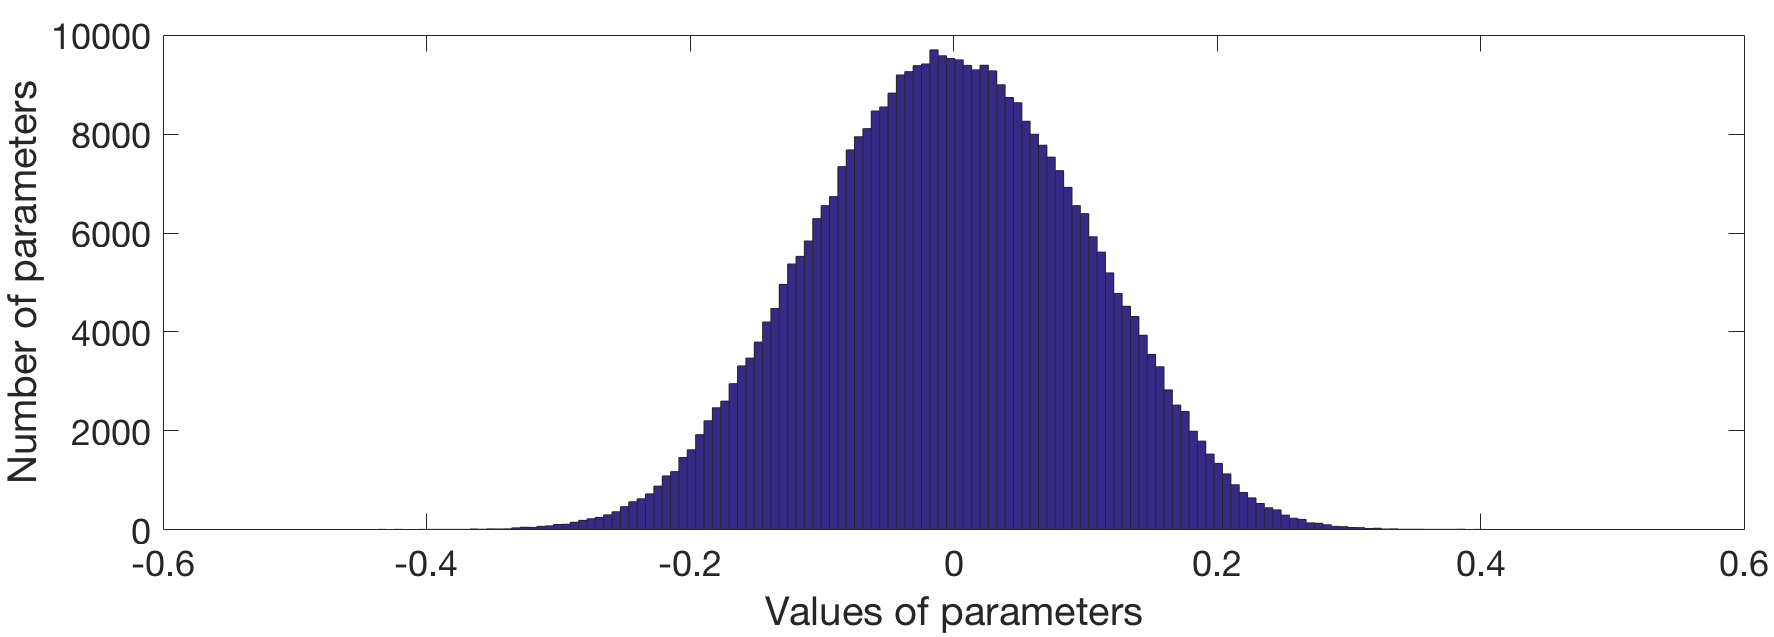
\includegraphics[width=\textwidth]{fig_unpruned.png}};
  \draw[latex-latex] (-5,0) -- (5,0) ; %edit here for the axis
  \foreach \x in {-0.6,-0.4,-0.2,0,0.2,0.4,0.6} % edit here for the numbers
  \draw[shift={(\x*10,0)},color=black] (-32pt,0pt) -- (-32pt,-3pt) node[below]
  {$\x$};
  % \draw[*-o] (0.92,0) -- (2.08,0);
  \draw[line width=8.8pt,color=red!10,shift={(-32pt,0)}] (-8,0) -- (8,0);
  \draw[line width=8.8pt,color=red!30,shift={(-32pt,0)}] (-5,0) -- (5,0);
  \draw[line width=8.8pt,color=red!40,shift={(-32pt,0)}] (-2.5,0) -- (2.5,0);
  \draw[line width=8.8pt,color=red!50,shift={(-32pt,0)}] (-1.25,0) -- (1.25,0);
  \draw[line width=8.8pt,color=red!60,shift={(-32pt,0)}] (-0.625,0) -- (0.625,0);
  \draw[line width=8.8pt,color=red!70,shift={(-32pt,0)}] (-0.313,0) -- (0.313,0);
  \draw[line width=8.8pt,color=red!80,shift={(-32pt,0)}] (-0.156,0) -- (0.156,0);
  \draw[line width=8.8pt,color=red!90,shift={(-32pt,0)}] (-0.078,0) -- (0.078,0);
  \draw[line width=8.8pt,color=red!100,shift={(-32pt,0)}] (-0.039,0) -- (0.039,0);
\end{tikzpicture}
\caption{Parameter distribution of the first fully connected layer in \textit{
LeNet5}, and the color coded arithmetic precisions using \textit{Customized floating-point quantization}
with $1$-bit sign, $1$-bit exponent and $3$-bit fraction.
A deeper red color corresponds to a greater arithmetic precision, the quantization is non-linear since
the representations is focused on a particular range.}
\label{fig:weight_dist_cfc}
\end{figure}
Previously, all quantization methods focused on unpruned networks and proved
good compression rates.
The high precision region of these applied arithmetics focuses on the center of
the weights distribution.

Given an example in \Cref{fig:weight_dist_cfc}, the chosen arithmetic has the
ability to represent numbers more precisely in the region where most weights
exist.
The color coded bar is deepest at values near zero, and the histogram
shows its peak at zero as well.
This partially explains why quantizations with dynamic ranges (
\textit{Customized floating-point} and \textit{Dynamic fixed-point}
) work well, because now greater precisions can be explored near zero.
However, for pruned models, the advantage of using dynamic ranges disappears.

\begin{figure}[!h]
\begin{tikzpicture}
\draw (-5,0.05) node[above] {\textbf{Color coded arithmetic precisions}};
% \draw (-5,0.2) node[] {High intensity};
% \draw[line width=4.8pt,color=red!100] (-5,0.15) -- (-4.1,0.15);
\node[anchor=south west,inner sep=0] at (-8.05,-6) {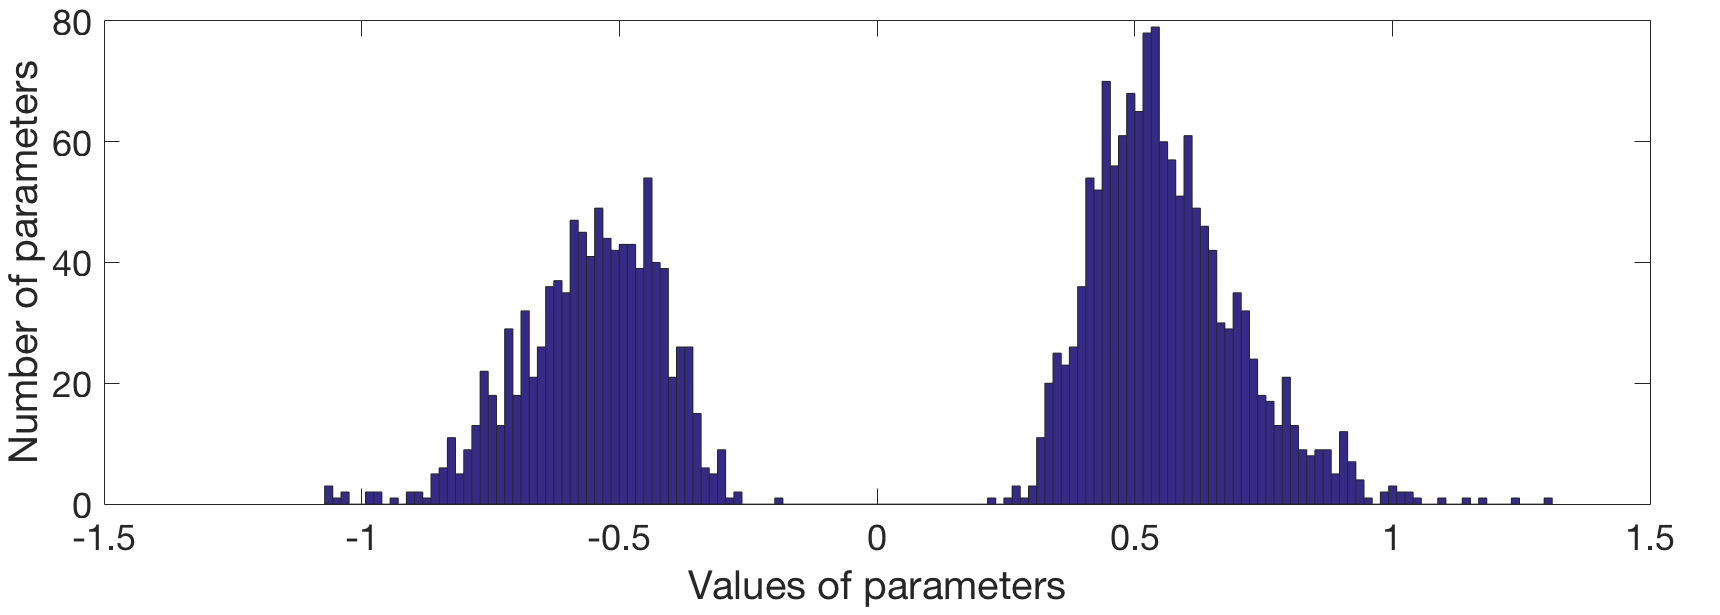
\includegraphics[width=\textwidth]{fig_pruned.png}};
% \draw[latex-latex] (-8,0) -- (8,0) ; %edit here for the axis
% \foreach \x in  {-3,-2,-1,0,1,2,3} % edit here for the vertical lines
% \draw[shift={(\x,0)},color=black] (0pt,3pt) -- (0pt,-3pt);
\foreach \x in {-1,-0.5,0,0.5,1} % edit here for the numbers
\draw[shift={(\x*4.1,0)},color=black] (-30pt,0pt) -- (-30pt,-3pt) node[below]
{$\x$};
% \draw[*-o] (0.92,0) -- (2.08,0);
\draw[line width=8.8pt,color=black!90,shift={(-30pt,0)}] (-0.039,0) -- (0.039,0);
\draw[line width=8.8pt,color=black!90,shift={(-30pt,0)}] (-0.039,0) -- (0.039,0);
\draw[line width=8.8pt,color=red!5,shift={(-30pt,0)}] (-8,0) -- (8,0);
\draw[line width=8.8pt,color=red!30,shift={(-30pt,0)}] (-5,0) -- (5,0);
\draw[line width=8.8pt,color=red!40,shift={(-30pt,0)}] (2-2.5,0) -- (2+2.5,0);
\draw[line width=8.8pt,color=red!40,shift={(-30pt,0)}] (-2-2.5,0) -- (-2+2.5,0);
\draw[line width=8.8pt,color=red!50,shift={(-30pt,0)}] (2-1.25,0) -- (2+1.25,0);
\draw[line width=8.8pt,color=red!50,shift={(-30pt,0)}] (-2-1.25,0) -- (-2+1.25,0);
\draw[line width=8.8pt,color=red!60,shift={(-30pt,0)}] (2-0.625,0) -- (2+0.625,0);
\draw[line width=8.8pt,color=red!60,shift={(-30pt,0)}] (-2-0.625,0) -- (-2+0.625,0);
\draw[line width=8.8pt,color=red!70,shift={(-30pt,0)}] (-2-0.313,0) -- (-2+0.313,0);
\draw[line width=8.8pt,color=red!70,shift={(-30pt,0)}] (2-0.313,0) -- (2+0.313,0);
\draw[line width=8.8pt,color=red!80,shift={(-30pt,0)}] (-2-0.156,0) -- (-2+0.156,0);
\draw[line width=8.8pt,color=red!80,shift={(-30pt,0)}] (2-0.156,0) -- (2+0.156,0);
\draw[line width=8.8pt,color=red!90,shift={(-30pt,0)}] (2-0.078,0) -- (2+0.078,0);
\draw[line width=8.8pt,color=red!90,shift={(-30pt,0)}] (-2-0.078,0) -- (-2+0.078,0);
\draw[line width=8.8pt,color=red!120,shift={(-30pt,0)}] (2-0.39,0) -- (2+0.039,0);
\draw[line width=8.8pt,color=red!120,shift={(-30pt,0)}] (-2-0.39,0) -- (-2+0.039,0);
\end{tikzpicture}
\caption{Parameter distribution of the first fully connected layer in \textit{
LeNet5}, and the color coded arithmetic precisions using \textit{Centralized customized floating-point quantization}
with $1$-bit sign, $1$-bit centre, $1$-bit exponent and $3$-bit fraction.
A deeper red color corresponds to a greater arithmetic precision, the quantization is non-linear since
the representations is focused on particular ranges.}
\label{fig:prune_dist}
\end{figure}

As shown in \Cref{fig:prune_dist}, the weights distribution has a binomial shape,
if the same arithmetic used before applies on this weights distribution,
the middle empty region will have the richest number representations.
The waste in number representation suggests that a suitable arithmetic for
pruned models should have the
ability to represent numbers that are away from zeros in high precisions.
The color coded arithmetic precision bar suggests the preferred precision
intensities.
The arithmetic should have high precision on two center points that are away
from zero, and have low precision representation for weights that are near zero
because these weights have been pruned away already.

\subsubsection{Method Description}
The methods introduced in this section is called \textit{Re-centralization}.
The shape of weights distribution of a pruned model is binomial, however, its
central values of two peaks can be different for every layer.
In this method, the weights parameters are inspected before quantization occurs and
two central values are determined layer-wise.
Two central values correspond to the two peaks of the binomial distribution
and are stored globally for parameters in the same layer.
For each layer, two central values are recorded and I use $1$ bit ($C$ bit) to
help a single parameter to determine which central value it is associated with.
This re-centralization technique is applied on both \textit{Dynamic fixed-point}
and \textit{Customized floating-point}.

\begin{figure}[!h]
\centering
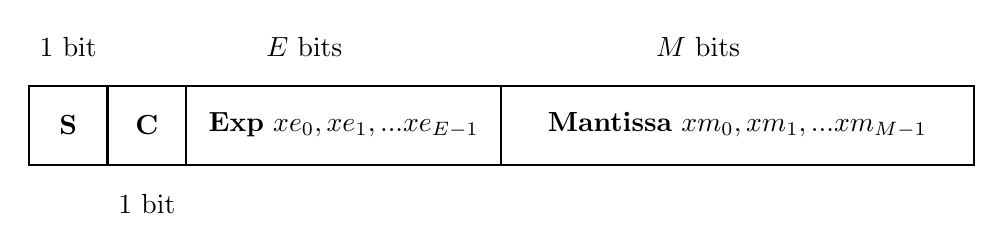
\begin{tikzpicture}
  \draw[style=thick] (0,0) rectangle (1,1) node(sign)[pos=.5] {\textbf{S}};
  \draw[style=thick] (1,0) rectangle (2,1) node(sign)[pos=.5] {\textbf{C}};
  \draw[style=thick] (2,0) rectangle (6,1) node(frac)[pos=.5] {\textbf{Exp} $xe_0, xe_1, ... xe_{E-1}$};
  \draw[thick] (6,0) rectangle (12,1) node(ignored)[pos=.5] {\textbf{Mantissa} $xm_0, xm_1, ... xm_{M-1}$};
  \node[] at (.5,1.5) {$1$ bit};
  \node[] at (1.5,-.5) {$1$ bit};
  \node[] at (3.5,1.5) {$E$ bits};
  \node[] at (8.5,1.5) {$M$ bits};
\end{tikzpicture}
\caption{Number representation system for \textit{Re-centralized customized floating-point quantization} with
1-bit sign, 1-bit central, E-bit exponent and M-bit mantissa.}
\label{fig:number_rep_ccfp}
\end{figure}

\begin{figure}[!h]
\centering
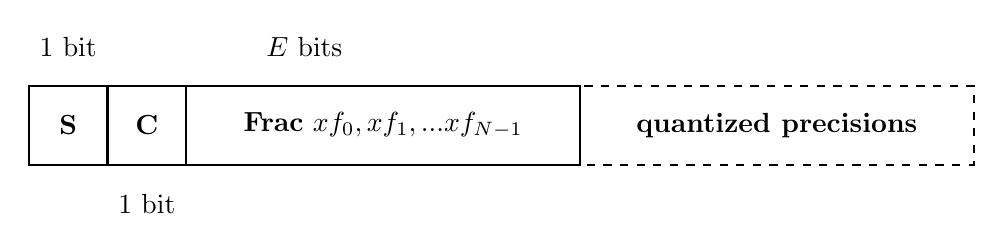
\begin{tikzpicture}
  \draw[style=thick] (0,0) rectangle (1,1) node(sign)[pos=.5] {\textbf{S}};
  \draw[style=thick] (1,0) rectangle (2,1) node(sign)[pos=.5] {\textbf{C}};
  \draw[style=thick] (2,0) rectangle (7,1) node(frac)[pos=.5] {\textbf{Frac} $xf_0, xf_1, ... xf_{N-1}$};
  \draw[thick,dashed] (7,0) rectangle (12,1) node(ignored)[pos=.5] {\textbf{quantized precisions}};
  \node[] at (.5,1.5) {$1$ bit};
  \node[] at (1.5,-.5) {$1$ bit};
  \node[] at (3.5,1.5) {$E$ bits};
\end{tikzpicture}
\caption{Number representation system for \textit{Re-centralized dynmaic fixed-point quantization} with
1-bit sign, 1-bit central and $N$-bit fraction.}
\label{fig:number_rep_cdfp}
\end{figure}

A \textit{Re-centralized customized floating-point} number representation system
is displayed in \Cref{fig:number_rep_ccfp},
the extra bit $C$ is also shown to determine which central value this parameter
belongs to.
Similarly, a \textit{Re-centralized dynmaic fixed-point} arithmetic is shown in
\Cref{fig:number_rep_cdfp}.
To convert from this \textit{Re-centralized customized floating-point} arithmetic to a normal decimal value, consider two
layer-wise central values to be $C_{pos}$ and $C_{neg}$.
The bit stored to identify the central value is $C$, we have:
\begin{equation}
    D = (-1)^S 2^{-\sum^{E-1}_{i=0}2^{-i}xe_i}(\sum^{M-1}_{i=0}2^{-i}xm_i) + (C C_{pos} + (1-C)C_{neg})
    % \caption{Decimal to fixed-point conversion}
    \label{equ:d2dfp}
\end{equation}

Similarly, \textit{Re-centralized customized floating-point} arithmetic can be converted
to the decimal representation using the equation below:
\begin{equation}
    D = (-1)^S 2^{-DR}(\sum^{N-1}_{i=0}2^{-i}xf_i) + (C C_{pos} + (1-C)C_{neg})
    % \caption{Decimal to fixed-point conversion}
    \label{equ:d2dfp}
\end{equation}

The re-centralization method achieves better compression results by quantizing in
a non-linear manner, which is similar to \textit{Weights sharing}.
As illustrated in \textit{Deep Compression} \cite{Han15}, \textit{Weights
sharing} clusters weights in a given layer and thus achieves nonlinear quantization.
\begin{figure}[!h]
  \centering
  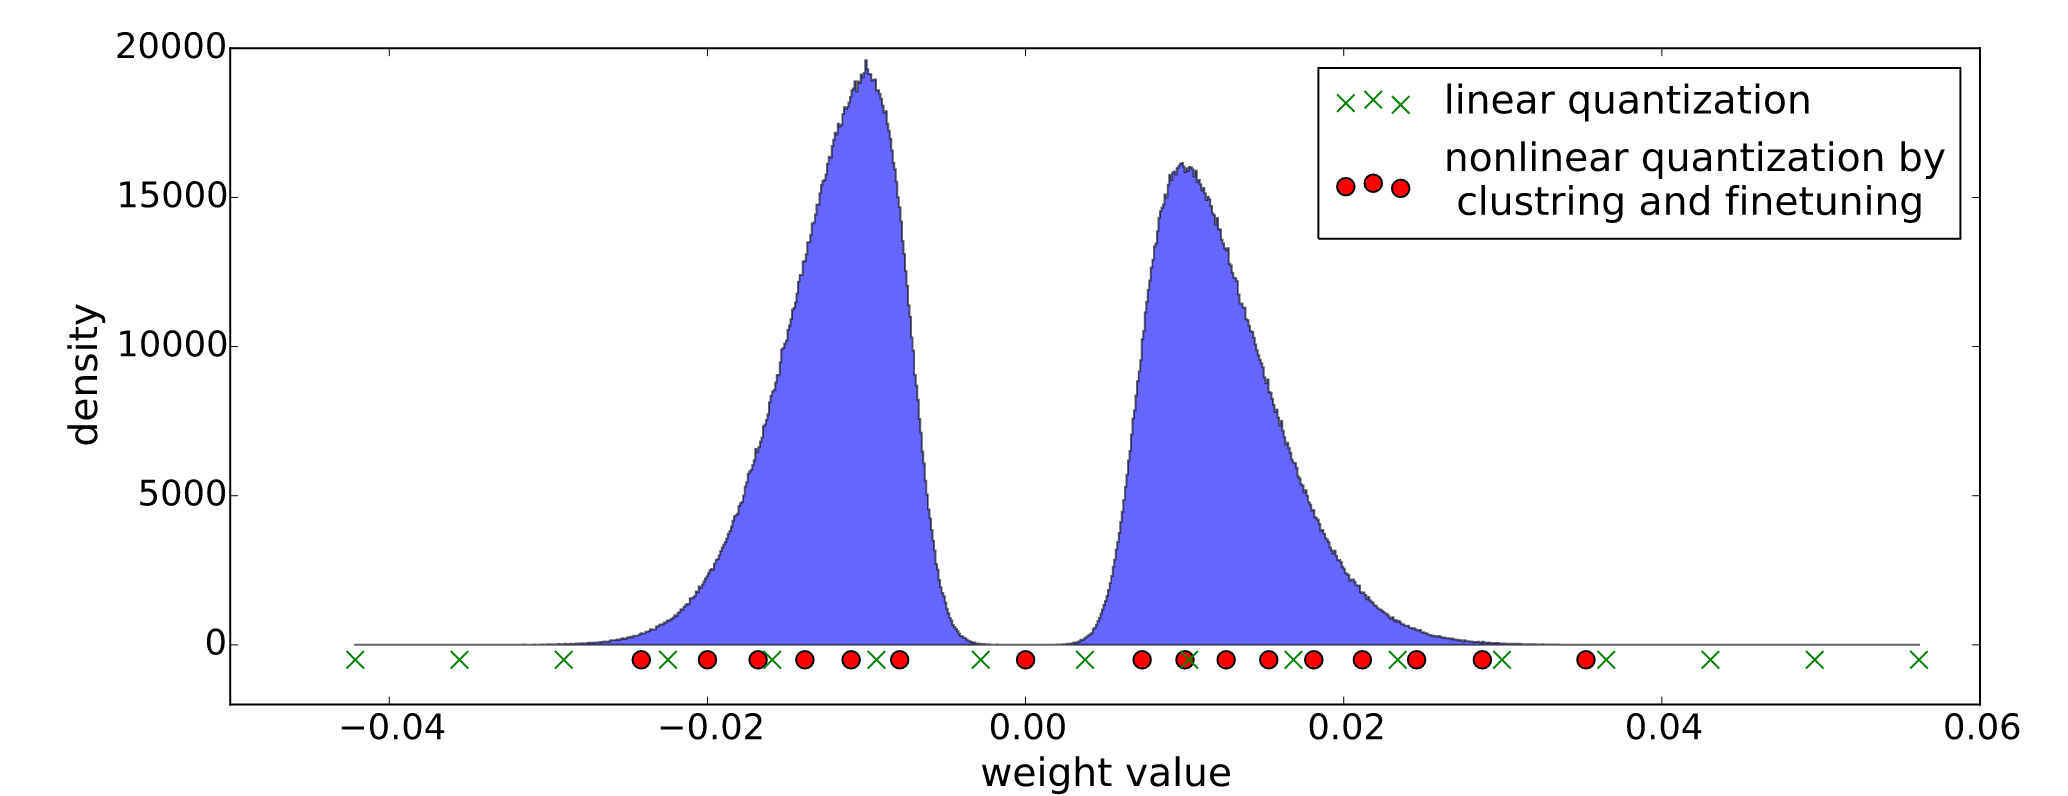
\includegraphics[width=\textwidth]{fig_weightsshare.png}%
  \caption{Distribution of weights (blue) and distribution of codebook
  before (green) and after \textit{Weights sharing}(red).}
  \label{fig:ws}
\end{figure}

\Cref{fig:ws} shows how \textit{Weights sharing} changes quantization to a
non-linear form, the quantized intensities are similar to \Cref{fig:prune_dist}.
In later sections, a complete comparision between the two compression pipelines
will demonstrate that re-centralization works as well as \textit{Weights sharing}.
Besides, re-centralization avoids clustering of weights and searching for weights
based on their indexes.
As mentioend previously, searching weights based on indexes might cause extra
data movements and thus reduces energy efficiency.

\subsubsection{Results}
To demonstrate the performance gain from re-centralization,
pruned models of both \textit{LeNet5} and \textit{CifarNet} are considered.
I show a comparison between
\textit{Customized floating-point quantization}, \textit{Centralized dynamic
fixed-point} and
\textit{Centralized customized floating-point} to observe the effects of
re-centralizations.
The results of quantization on a pruned \textit{LeNet5} are shown in
\Cref{tab:pruned_quan1}, and \Cref{tab:pruned_quan2} shows the quantization
results on pruned \textit{CifarNet}.

\begin{table}[!h]
  \centering
  \begin{tabular}{lllllll}
    \hline
    \hline
    Bit width               &32-bit     &16-bit       &8-bit       &6-bit     &4-bit\\
    \hline
    \hline
    \multicolumn{5}{l}{\textbf{\textit{LeNet5}}, \textit{Customized floating-point}}\\
    \hline
    Before Retrain          &99.36\%    &99.36\%      &99.31\%     &98.40\%   &73.94\%\\
    After Retrain           &99.36\%    &99.36\%      &99.36\%     &99.36\%   &99.36\%\\
    \hline
    \hline
    \multicolumn{5}{l}{\textbf{\textit{LeNet5}}, \textit{Centralized dynamic fixed-point}}\\
    \hline
    Before Retrain          &99.04\%    &99.04\%    &99.06\%     &98.93\%   &91.86\%\\
    After Retrain           &99.36\%    &99.36\%    &99.36\%     &99.36\%   &99.36\%\\
    \hline
    \hline
    \multicolumn{5}{l}{\textbf{\textit{LeNet5}}, \textit{Centralized customized floating-point}}\\
    \hline
    Before Retrain          &98.73\%    &98.72\%    &98.67\%     &98.04\%   &21.81\%\\
    After Retrain           &99.36\%    &99.36\%    &99.36\%     &99.36\%   &99.36\%\\
    \hline
    \hline
  \end{tabular}
  \caption{Quantization summary on a pruned \textit{LeNet5} model. \textit{Customized
  floating-point} has 1-bit sign, 1-bit exponent and the rest are mantissa bits.
  \textit{Centralized customized floating-point} has 1-bit sign, 1-bit central,
  1-bit exponent and the rest are mantissa bits.
  \textit{Centralized dynamic fixed-point} has
  1-bit sign, 1-bit central and the rest are fraction bits.}
  \label{tab:pruned_quan1}
\end{table}

As shown in \Cref{tab:pruned_quan1}, \textit{Customized floating-point} arithmetic
has a similar post-retrain accuracy to both \textit{Centralized customized floating-point}
and \textit{Centralized dynamic fixed-point} on \textit{LeNet5}.
However, the pre-retrain results of using \textit{Centralized dynamic fixed-point}
is actually the best one in these three arithmetics.
The limited mantissa width causes \textit{Centralized customized floating-point} to
have a bad pre-train accuracy.
The pre-train accuracy of this simple network is tightly linked to the number of
mantissa (or fractional) bits available.
The underlying issue is that \textit{LeNet5} is too simple, it seems
like a large precision near the central values would not introduce critical
improvements when no retraining takes place.
Another problem with this simple \textit{LeNet5} network is that all
arithmetics can achieve the same post-train accuracies, and lower precisions
cannot be explored because the sign bit and exponent bits set a minimum total bit width.

\begin{table}[!h]
  \centering
  \begin{tabular}{lllllll}
    \hline
    \hline
    Bit width               &32-bit     &16-bit     &8-bit      &6-bit    \\
    \hline
    \hline
    \multicolumn{5}{l}{\textbf{\textit{CifarNet}}, \textit{Customized floating-point}}\\
    \hline
    Before Retrain          &34.30\%    &29.19\%    &30.58\%    &20.56\%\\
    After Retrain           &82.02\%    &82.01\%    &81.85\%    &81.12\%\\
    \hline
    \hline
    \multicolumn{5}{l}{\textbf{\textit{CifarNet}}, \textit{Centralized dynamic fixed-point}}\\
    \hline
    Before Retrain          &81.18\%    &81.17\%    &80.06\%    &73.23\%\\
    After Retrain           &82.02\%    &82.06\%    &82.05\%    &82.10\%\\
    \hline
    \hline
    \multicolumn{5}{l}{\textbf{\textit{CifarNet}}, \textit{Centralized customized floating-point}}\\
    \hline
    Before Retrain          &59.65\%    &59.61\%   &58.23\%     &44.94\%\\
    After Retrain           &82.01\%    &82.11\%   &82.00\%     &81.79\%\\
    \hline
    \hline
  \end{tabular}
  \caption{Quantization summary on a pruned \textit{CifarNet} model. \textit{Customized
  floating-point} has 1-bit sign, 2-bit exponent and the rest are mantissa bits.
  \textit{Centralized customized floating-point} has 1-bit sign, 1-bit central,
  2-bit exponent and the rest are mantissa bits.
  \textit{Centralized dynamic fixed-point} has
  1-bit sign, 1-bit central and the rest are fraction bits.}
  \label{tab:pruned_quan2}
\end{table}


\Cref{tab:pruned_quan2} shows the quantization resutls when various
quantization methods are applied on the
pruned \textit{CifarNet}, \textit{Centralized customized floating-point}
and \textit{Centralized dynamic fixed-point} shows a significant improvement in
pre-train accuracy compared to \textit{Customized floating-point}.
Conceptually, centralized arithmetics re-focus the arithmetic centers to fit
the binomial weights distributions, and this should increase the precisions near central
values.
Using \textit{Centralized customized floating-point} on \textit{CifarNet}, it achieves the reqruied
accuracy at a precision of only $6$ bits.

\section{Summary of Quantization Methods}
To summarize, I would like
to compare the implemented quantization methods on the targeting networks.

Consider unpruned \textit{LeNet5} and \textit{CifarNet} as targeting networks,
\Cref{tab:quantize_summary}
shows the bit-widths of various networks after quantizations.
As mentioned previously, \textit{Dynamic fixed-point} (\textit{DFP}) restricts
the range of weights and thus some weights can never have a chance to recover.
As shown in the table, the error rate of using \textit{Dynamic fixed-point} is
slightly higher on \textit{LeNet5} due to this effect.
In contrast, \textit{CifarNet} shows comparable quantization results for both
\textit{Dynamic fixed-point} and \textit{Customized floating-point} (\textit{CFP}).
\textit{Gysel et al.} obtained their best quantization results using \textit{Dynamic fixed-point} on the unpruned
\textit{LeNet5} and \textit{CifarNet}, I added their results to \Cref{tab:quantize_summary}.

For quantizing unpruned models, \textit{Customized floating-point}
shows best results on the two selected networks: it showed a good compression
rates on both networks without any loss of test accuracies.

\begin{table}[!h]
  \centering
  \begin{tabular}{lllll}
    \hline
    Model             & \textit{Fixed-point}  &\textit{DFP}   &\textit{CFP}   &(\textit{Gysel})\\
    \hline
    \hline
    \textit{LeNet5}   & 16 bits($0.64\%$)     &4 bits($0.69\%$)              &4 bits($0.64\%$)   & 4 bits($0.90\%$)\\
    \textit{CifarNet} & 32 bits($18\%$)      &8 bits($18\%$ )              &8 bits($18\%$)   & 8 bits($18.3\%$)\\
    \hline
    \hline
  \end{tabular}
  \caption{Quantization summary (bit-width, error rate) on unpruned
  \textit{LeNet5} and \textit{CifarNet}. \textit{DFP} is \textit{Dynamic fixed-point},
  \textit{CFP} is \textit{Customized floating-point} and (\textit{Gysel}) is
  \textit{Gysel et al.}'s implemenetation of \textit{Dynamic fixed-point} \cite{Gysel}.}
  \label{tab:quantize_summary}
\end{table}

Quantization on pruned networks works differently from the unpruned ones.
As illustrated before, pruned network have central values that are non-zeros.
Re-centralization significantly helps number representation systems to focus
on the region with a large number of parameters using only one extra central bit.
Two re-centralization methods, named \textit{Centralized customized floating-point}
(\textit{CCFP}) and \textit{Centralized dynamic fixed-point} (\textit{CDFP}) respectively, are
applied on the pruned networks.
\Cref{tab:quantize_summary2} shows the quantization results, both arithmetics
achieve same quantization results on the pruned \textit{LeNet5} model, but
\textit{Centered dynamic fixed-point} shows a better performance on
the pruned \textit{CifarNet} model by achieving zero accuracy loss using only
$6$ bits.

\begin{table}[!h]
  \centering
  \begin{tabular}{llll}
    \hline
    Model             &\textit{CFP}     &\textit{CCFP}    &\textit{CDFP}\\
    \hline
    \hline
    \textit{LeNet5}   &4 bits($0.64\%$)  &4 bits($0.64\%$)  &4 bits($0.64\%$)\\
    \textit{CifarNet} &8 bits($18.2\%$) &8 bits($18\%$)   &6 bits($18\%$)\\
    \hline
    \hline
  \end{tabular}
  \caption{Quantization summary (bit-width, error rate) on pruned \textit{LeNet5}
  and \textit{CifarNet}. \textit{CFP} is \textit{Customized floating-point}
  \textit{CCFP} is \textit{Centralized customized floating-point} and
  \textit{CDFP} is \textit{Centralized dynmaic fixed-point}.
  }
  \label{tab:quantize_summary2}
\end{table}


% \centering
%   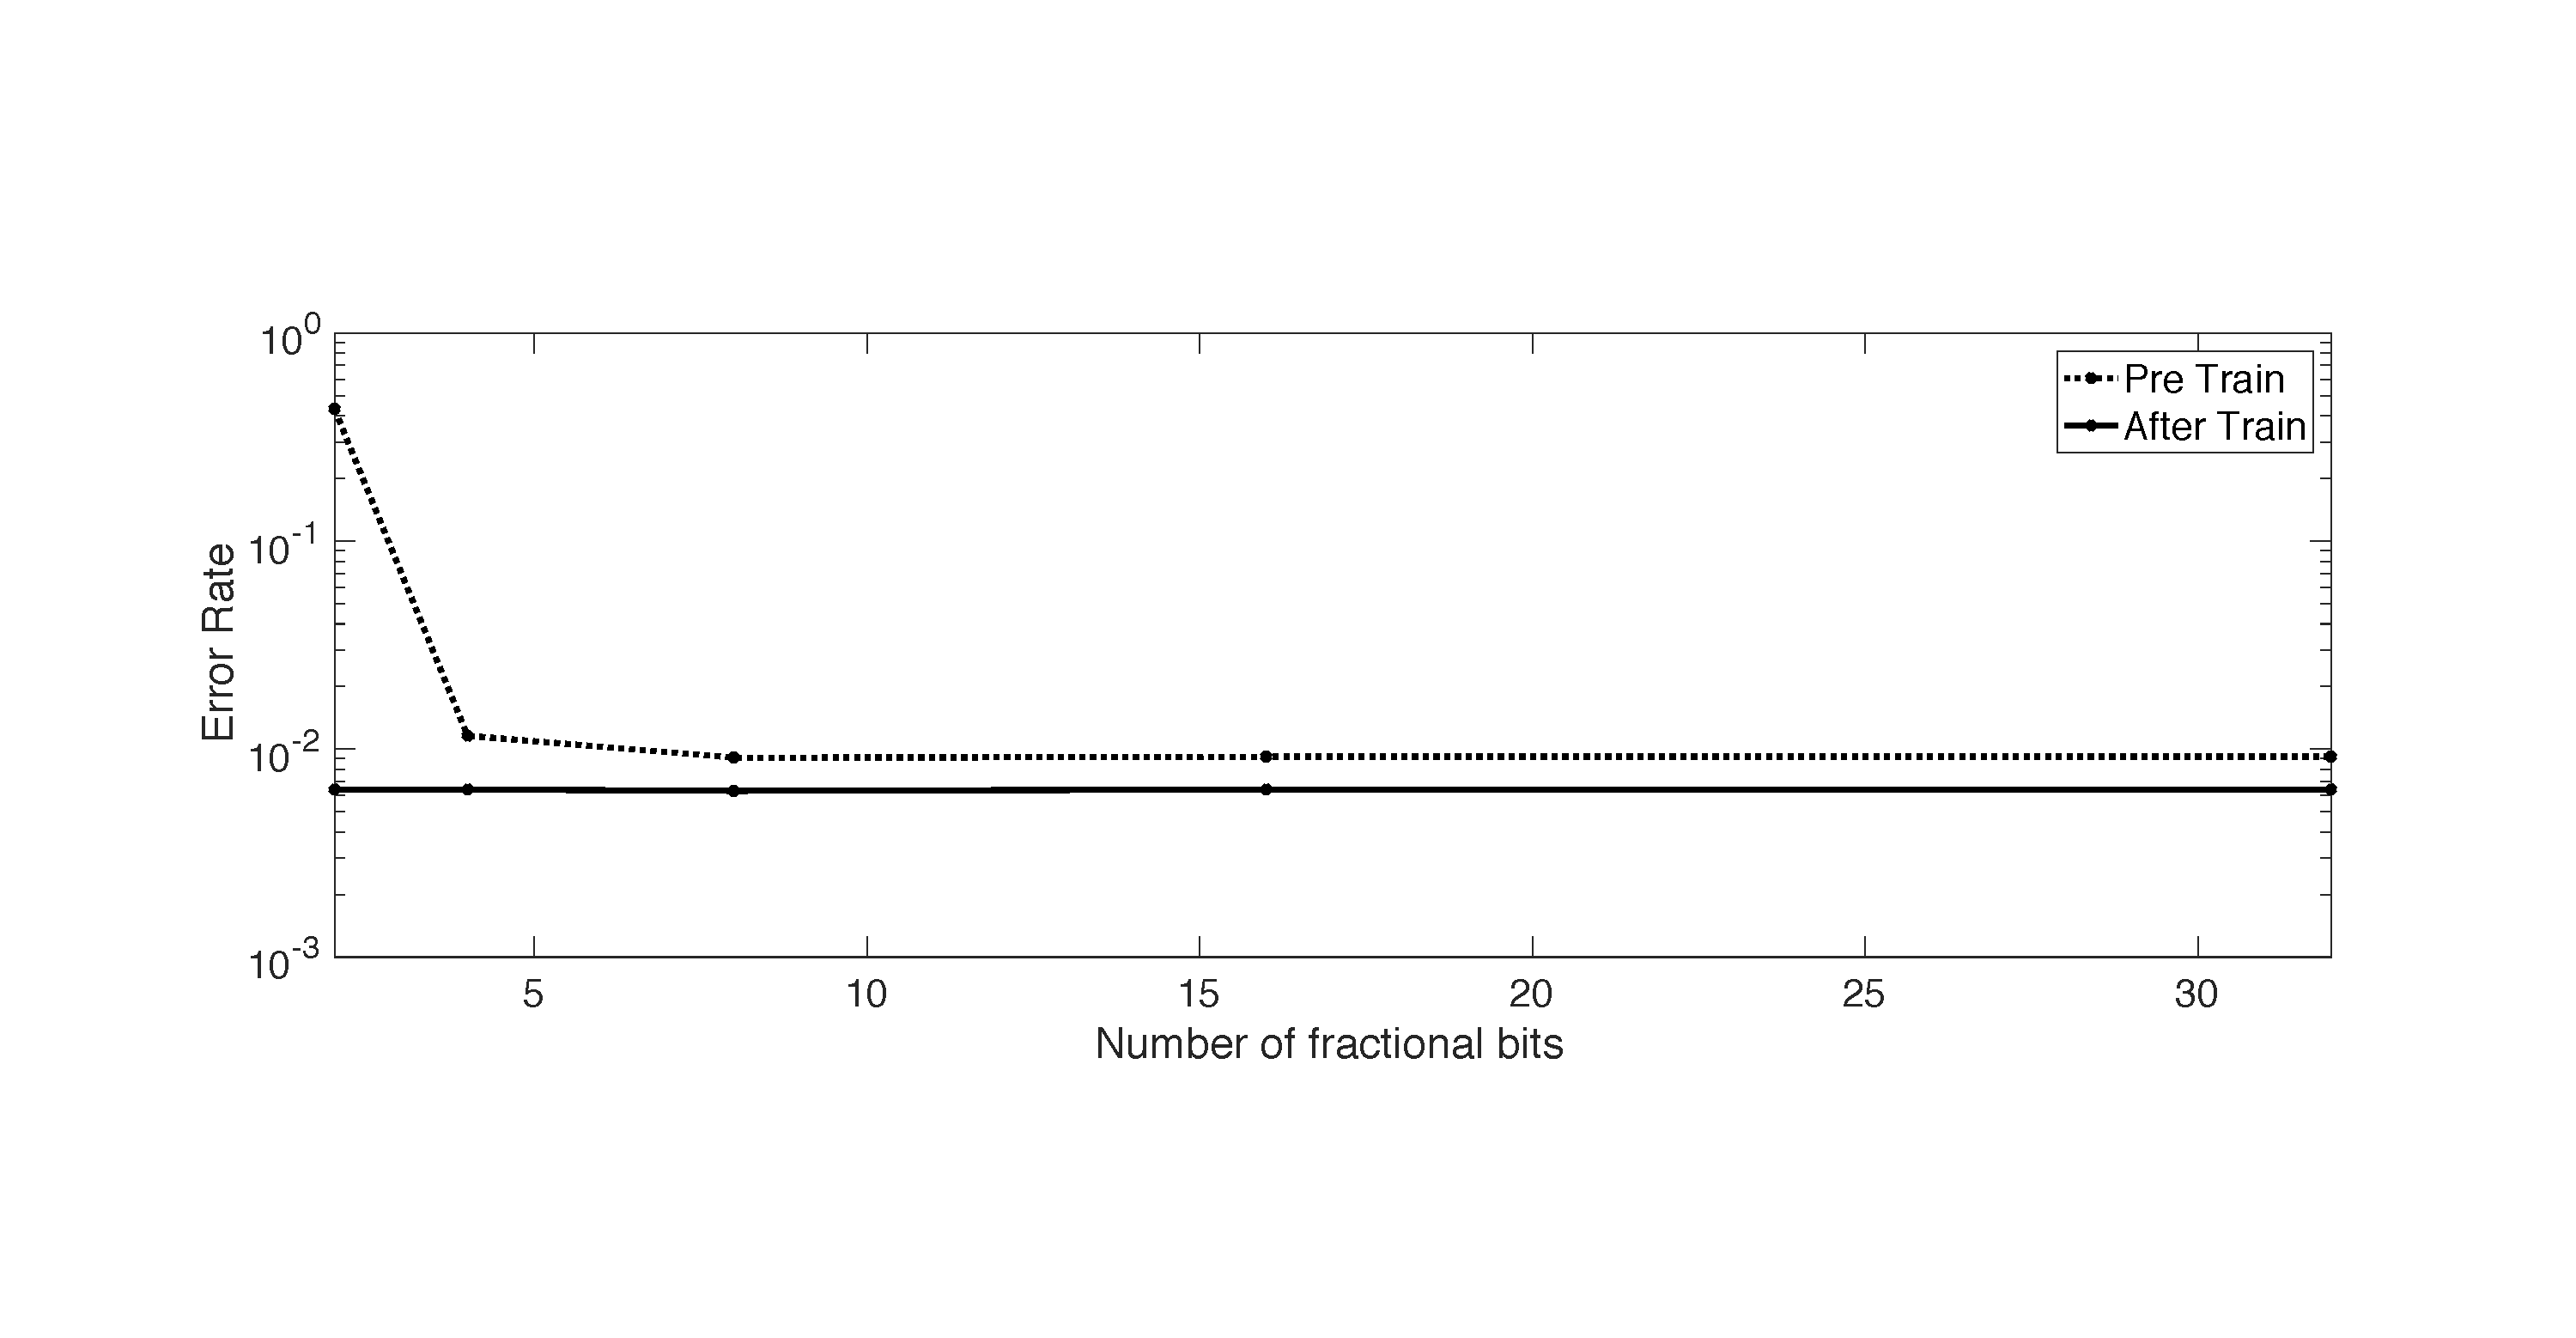
\includegraphics[width=\textwidth]{LeNet5_dynamic_fp.pdf}%
%   \label{fig:LeNetdfp}
%   \caption{Test accuracies for LetNet5 using dynamic fixed-point quantization.}
% \end{figure}
% \begin{figure}[!h]
% \centering
%   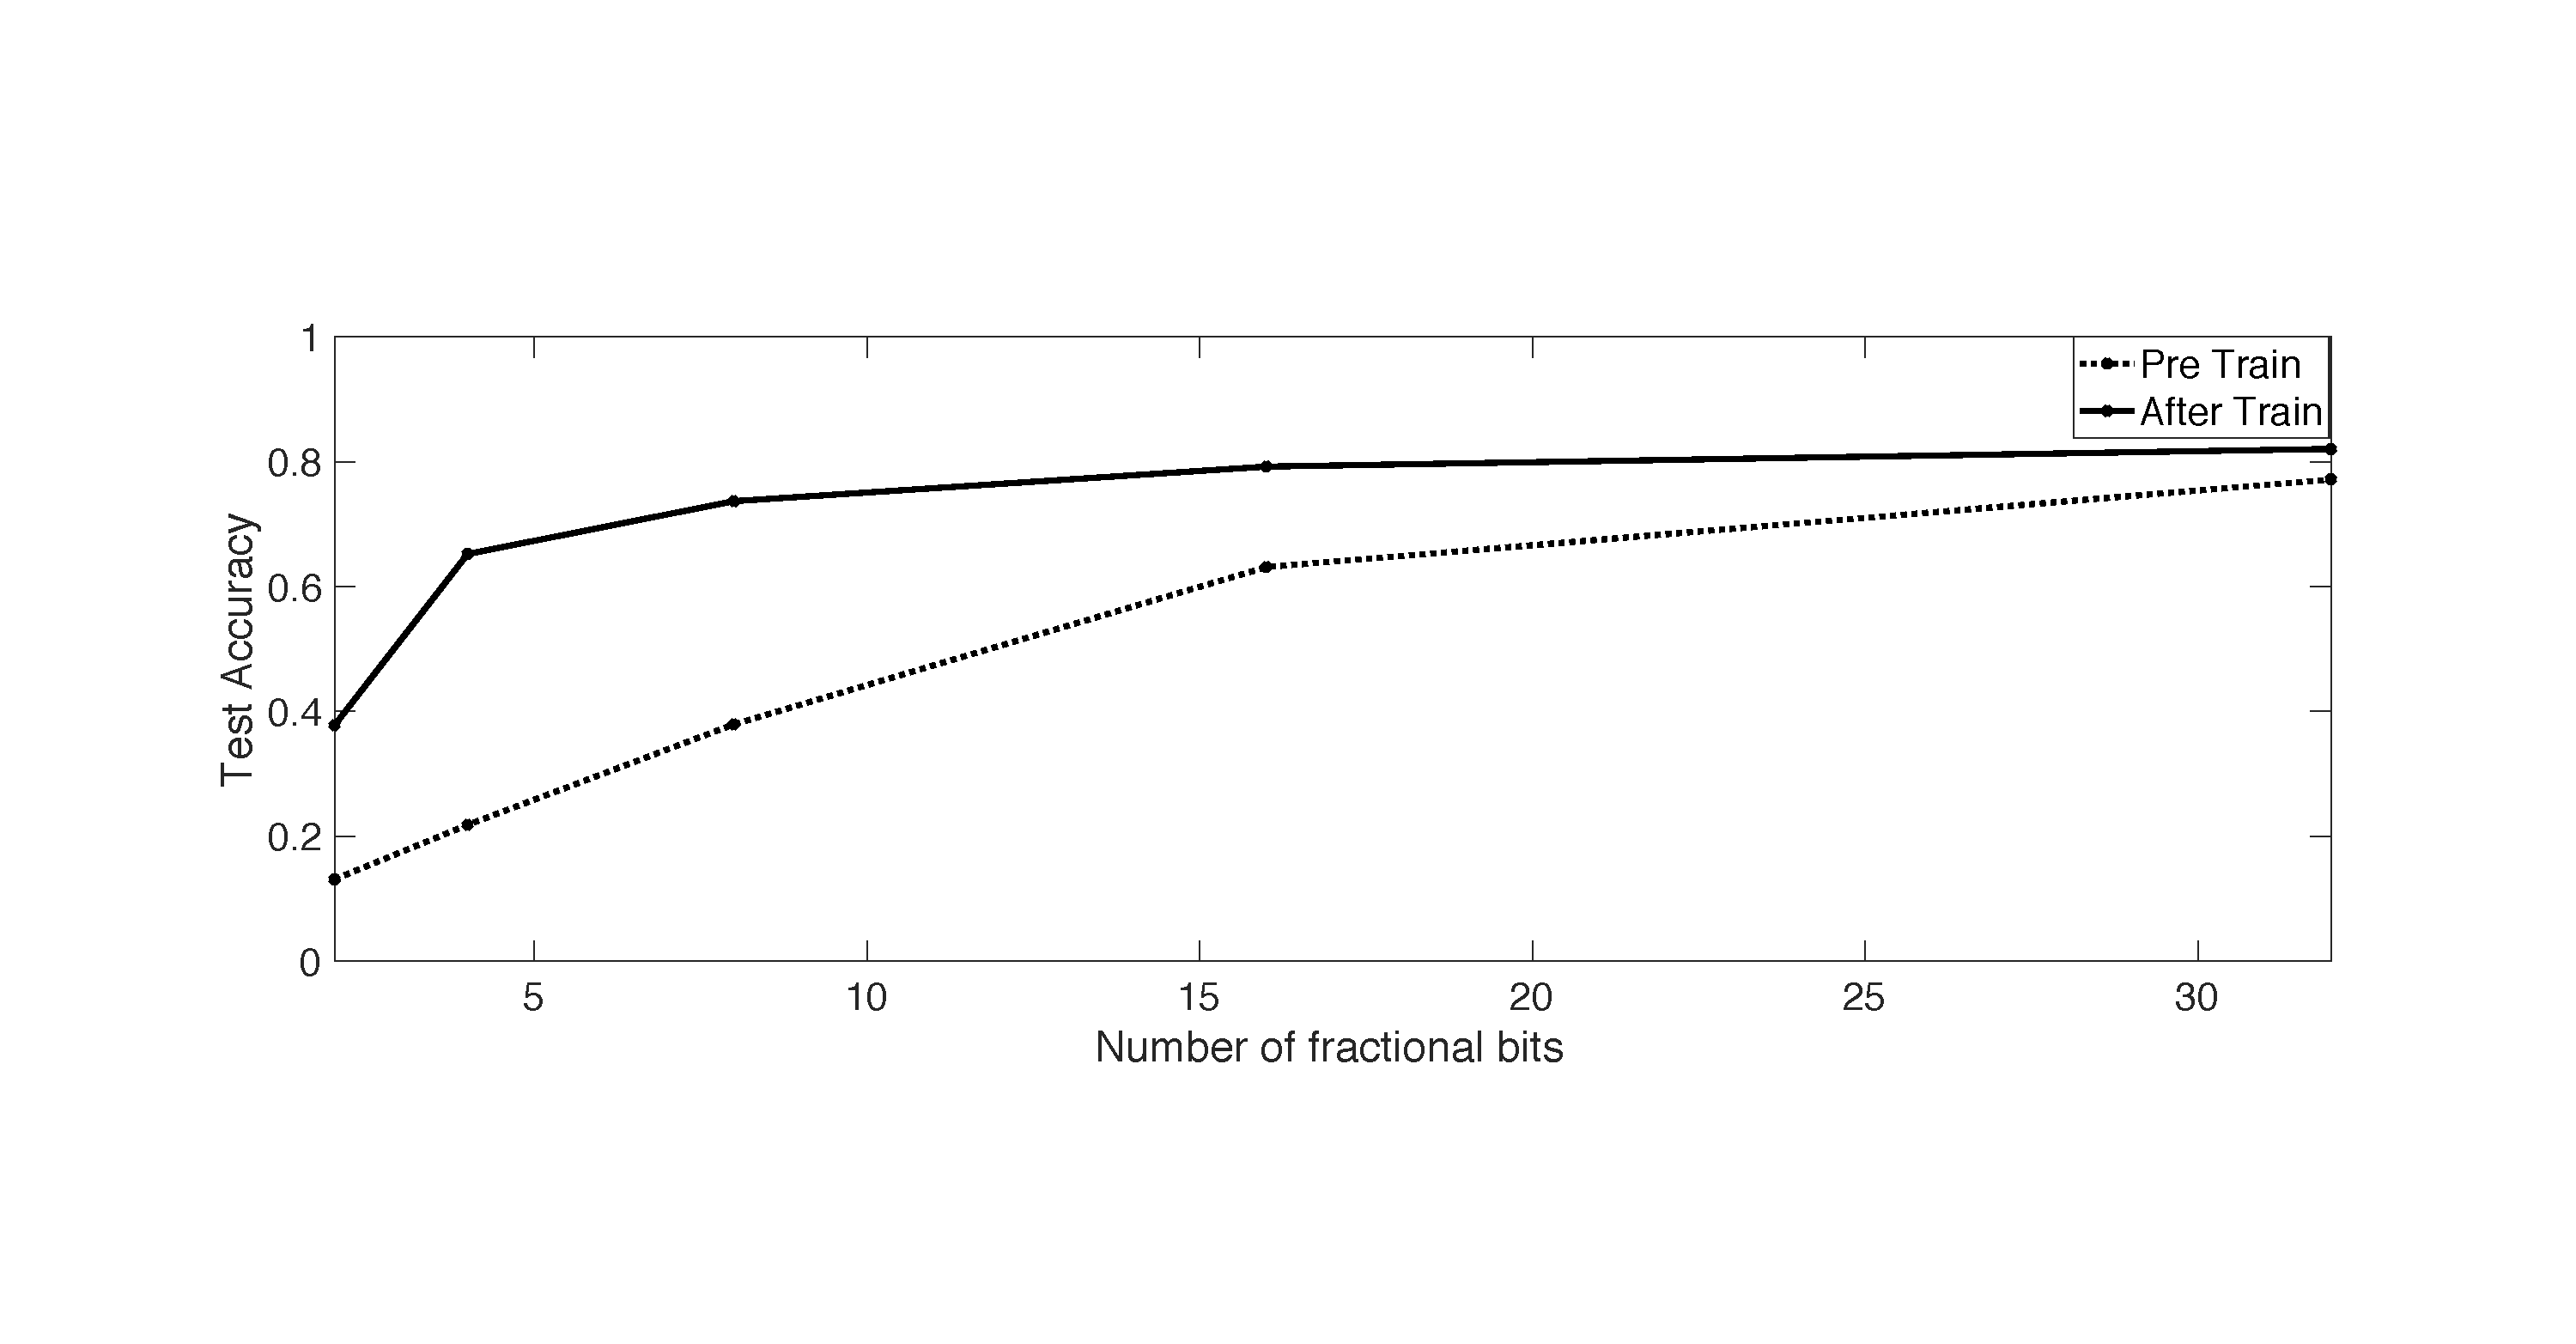
\includegraphics[width=\textwidth]{CifarNet_dfp.pdf}%
%   \label{fig:LeNetdfp}
%   \caption{Test accuracies for CifarNet using dynamic fixed-point quantization.}
% \end{figure}
%
% \begin{figure}[!h]
% \centering
%   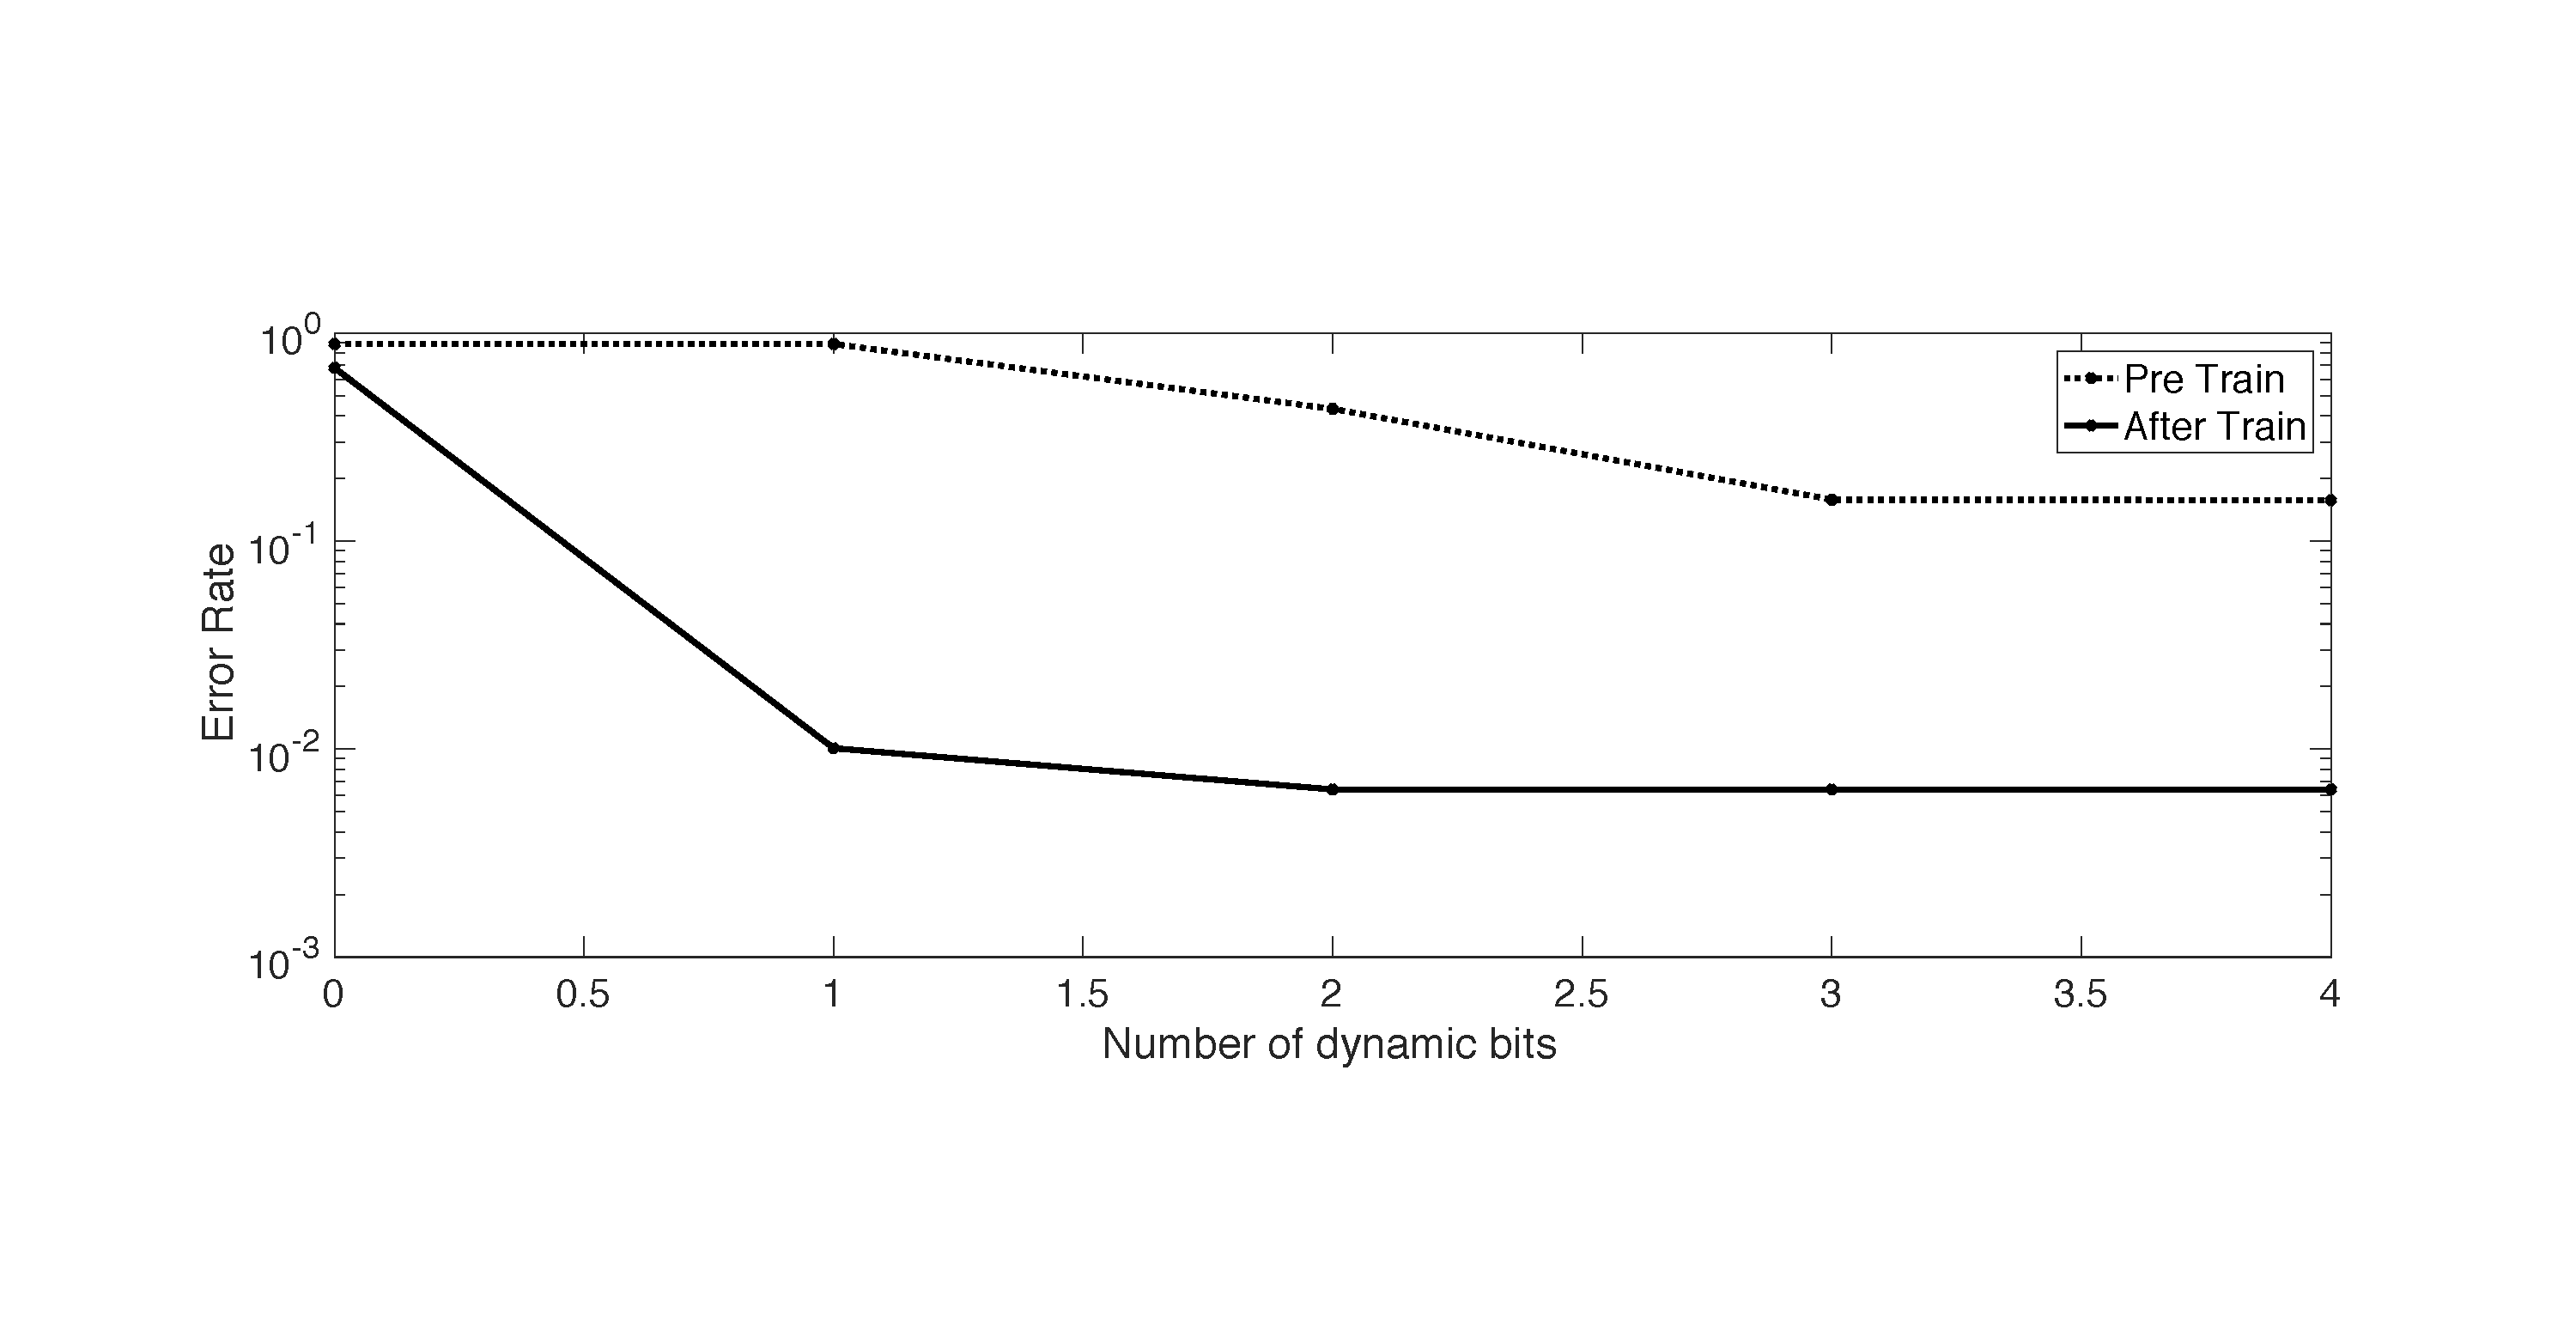
\includegraphics[width=\textwidth]{LeNet5_dynamic_fp_drange.pdf}%
%   \label{fig:LeNetdfp}
%   \caption{Test accuracies for LetNet5 using dynamic fixed-point quantization on various dynamic ranges.}
% \end{figure}
\chapter{Evaluation}
\section{Compression Pipeline}
\textit{Han et al.} proposed a three-stage compression pipeline called
\textit{Deep Compression}.
This work is most comparable to my compression pipeline.
Other research works almost focus only on whether pruning or quantization in an
isolated manner.
In this section, I would like to compare my compression pipeline to \textit{Deep Compression}

As shown in \Cref{fig:deep_compression_flow}, \textit{Han et al.} focused on
reducing the number of parameters first using \textit{Deterministic pruning} iteratively.
This iterative pruning process is combined with retraining to bring back the lost
accuracies.
They then utilized both \textit{Fixed-point quantization} and \textit{Weights sharing}
to minimize the number representation of each individual parameter.
Weights are quantized to limited precisions and encoded using a codebook
to reduce the amount of representations.
Finally, they tried to compress the number representations further using an
encoding scheme \cite{Han15}.

\textit{Deep Compression} is proven successful on many popular neural networks.
To give a fair comparison between my compression pipeline and \textit{Deep Compression},
the encoding stage is not considered for two reasons.
First, encoding schemes normally encode symbols by their occurrences, such an encoding
scheme can be attached to the end of any compression pipelines.
Second, the use of encoding indicates a need for encoder and decoder in hardware,
this might affect energy efficiency of the hardware platform.
\begin{figure}[!h]
  % \begin{tikzpicture}[thick]
  %   \node[draw,box] (a) {Deterministic Pruning};
  %   \node[draw,box,right=1cm of a] (b) {Quantization and Weights Sharing};
  %   \node[draw,box,right=1cm of b] (c) {Huffman Encoding};
  %   \draw[ultra thick,->] (a) -- (b);
  %   \draw[ultra thick,->] (b) -- (c);
  % \end{tikzpicture}

  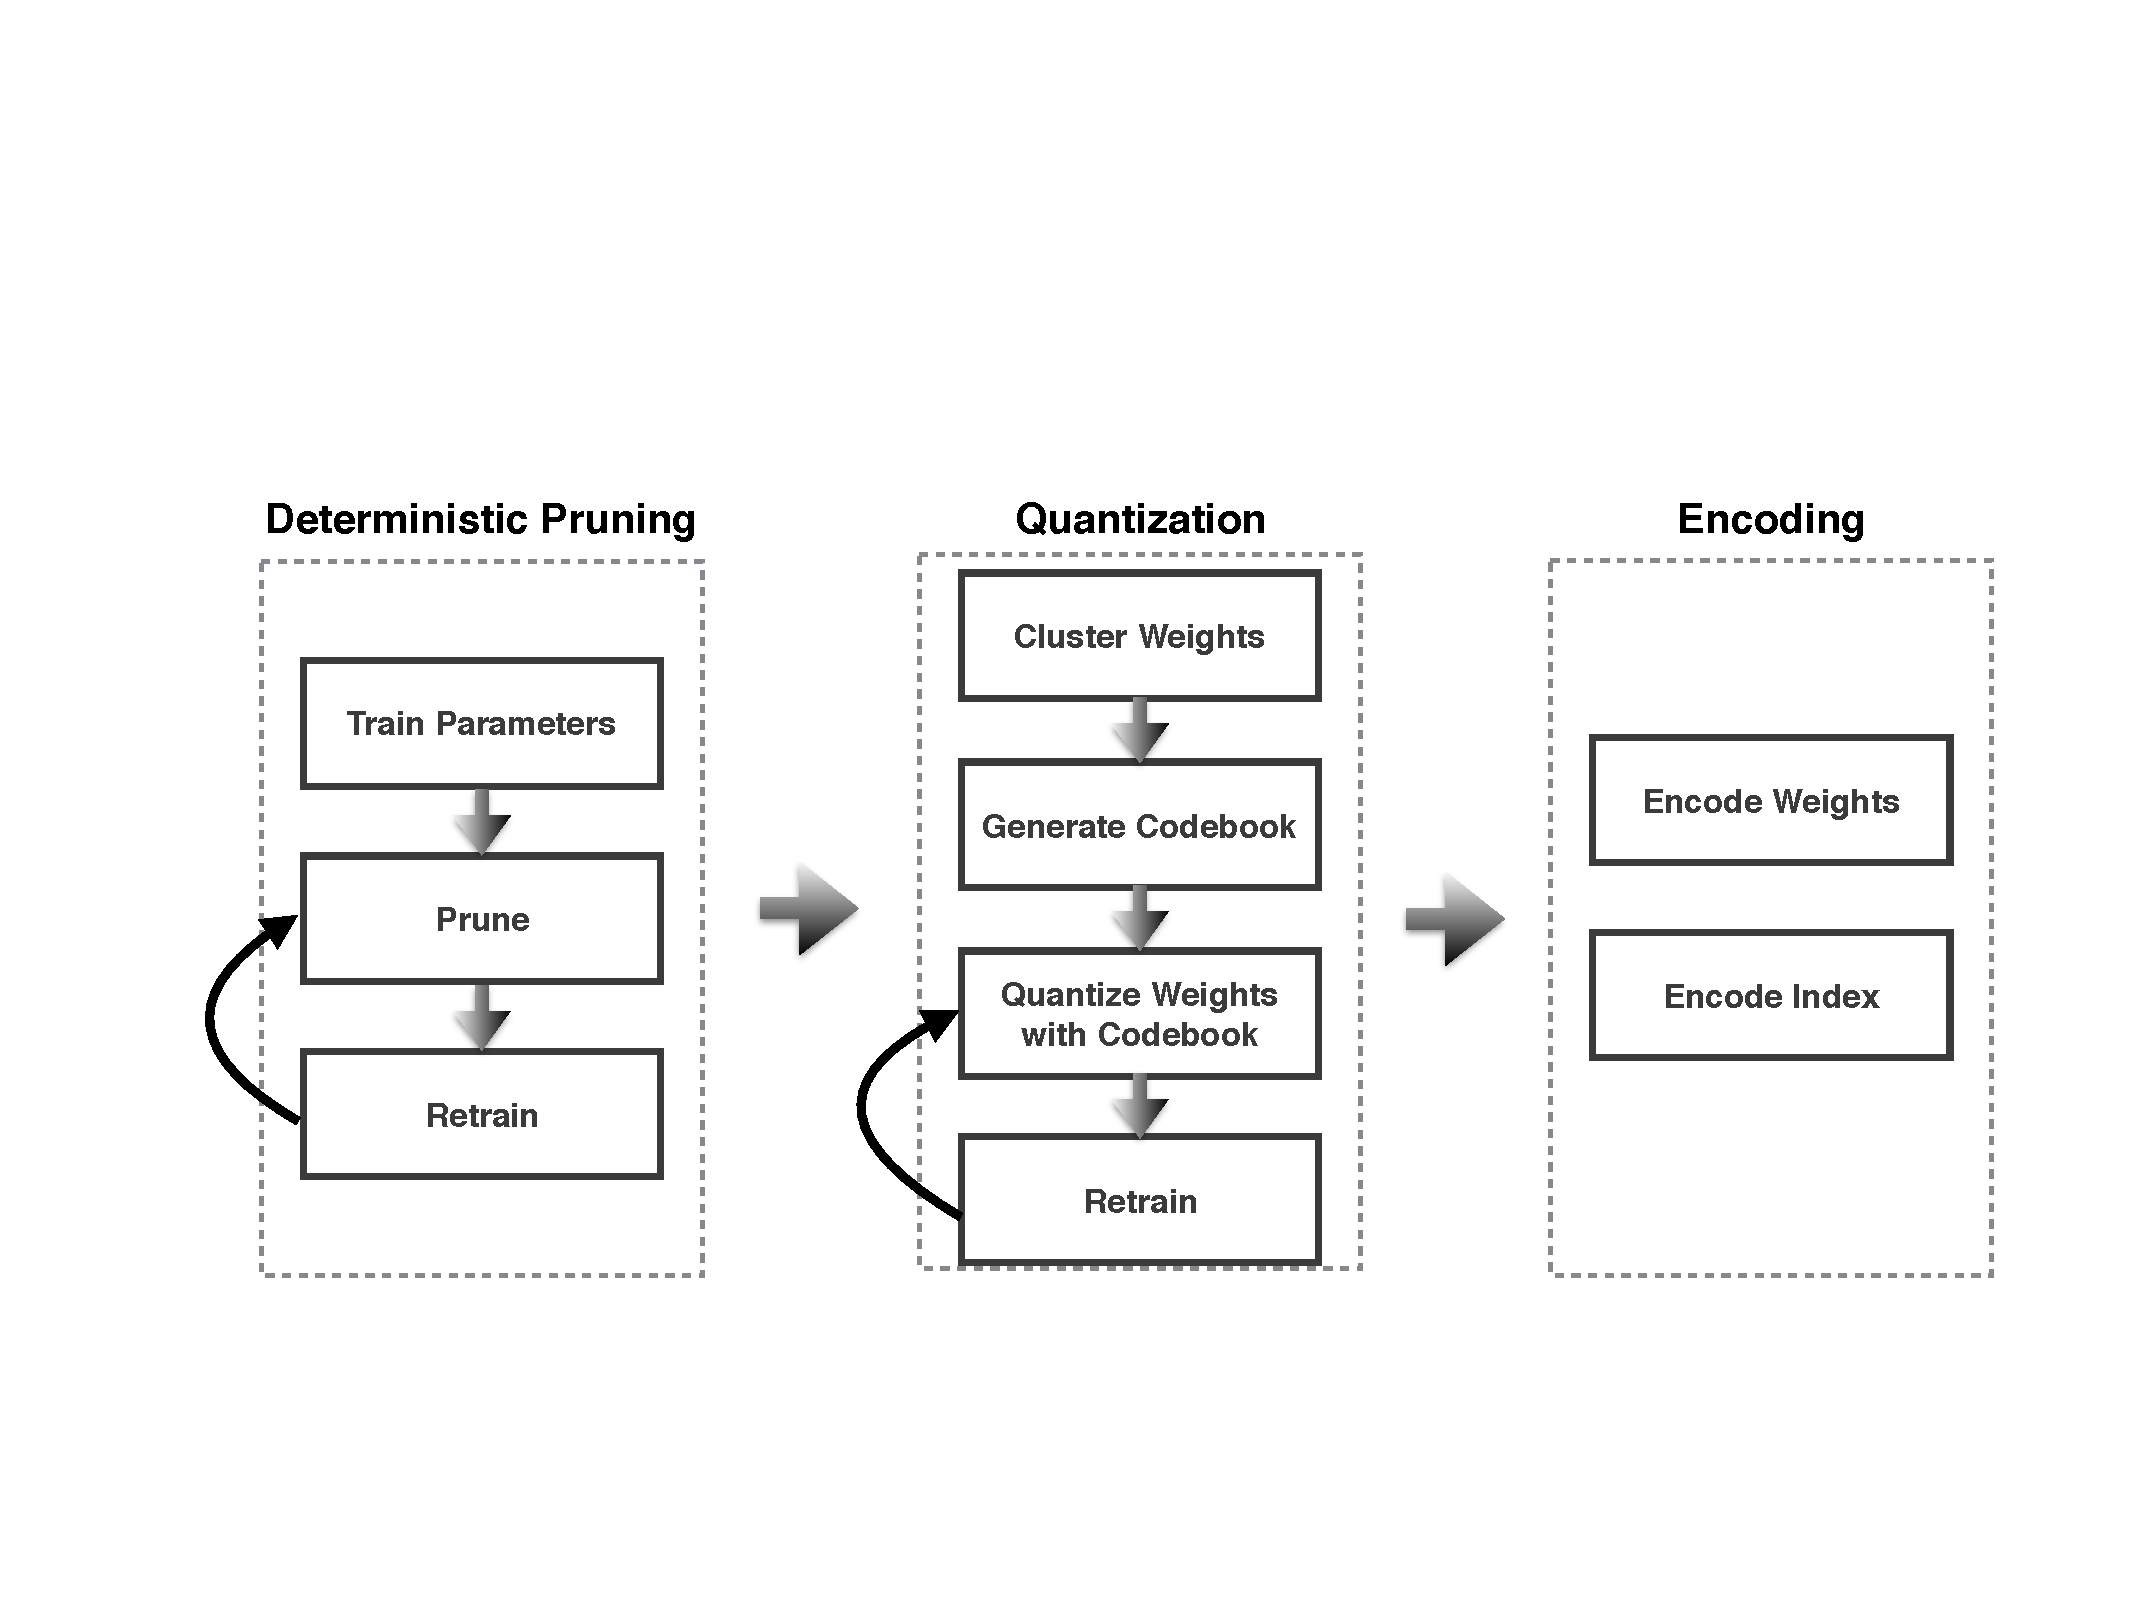
\includegraphics[width=\textwidth]{fig_dc.pdf}
  \caption{Overview of \textit{Deep Compression} \cite{Han15}.}
  \label{fig:deep_compression_flow}
\end{figure}
\begin{figure}[!h]
  % \begin{tikzpicture}[thick]
  %   \node[draw,box] (a) {Dynamic network surgery};
  %   \node[draw,box,right=1cm of a] (b) {L1/L2 Regularizer};
  %   \node[draw,box,right=1cm of b] (c) {Dynamic Fixed Point};
  %   \draw[ultra thick,->] (a) -- (b);
  %   \draw[ultra thick,->] (b) -- (c);
  % \end{tikzpicture}
  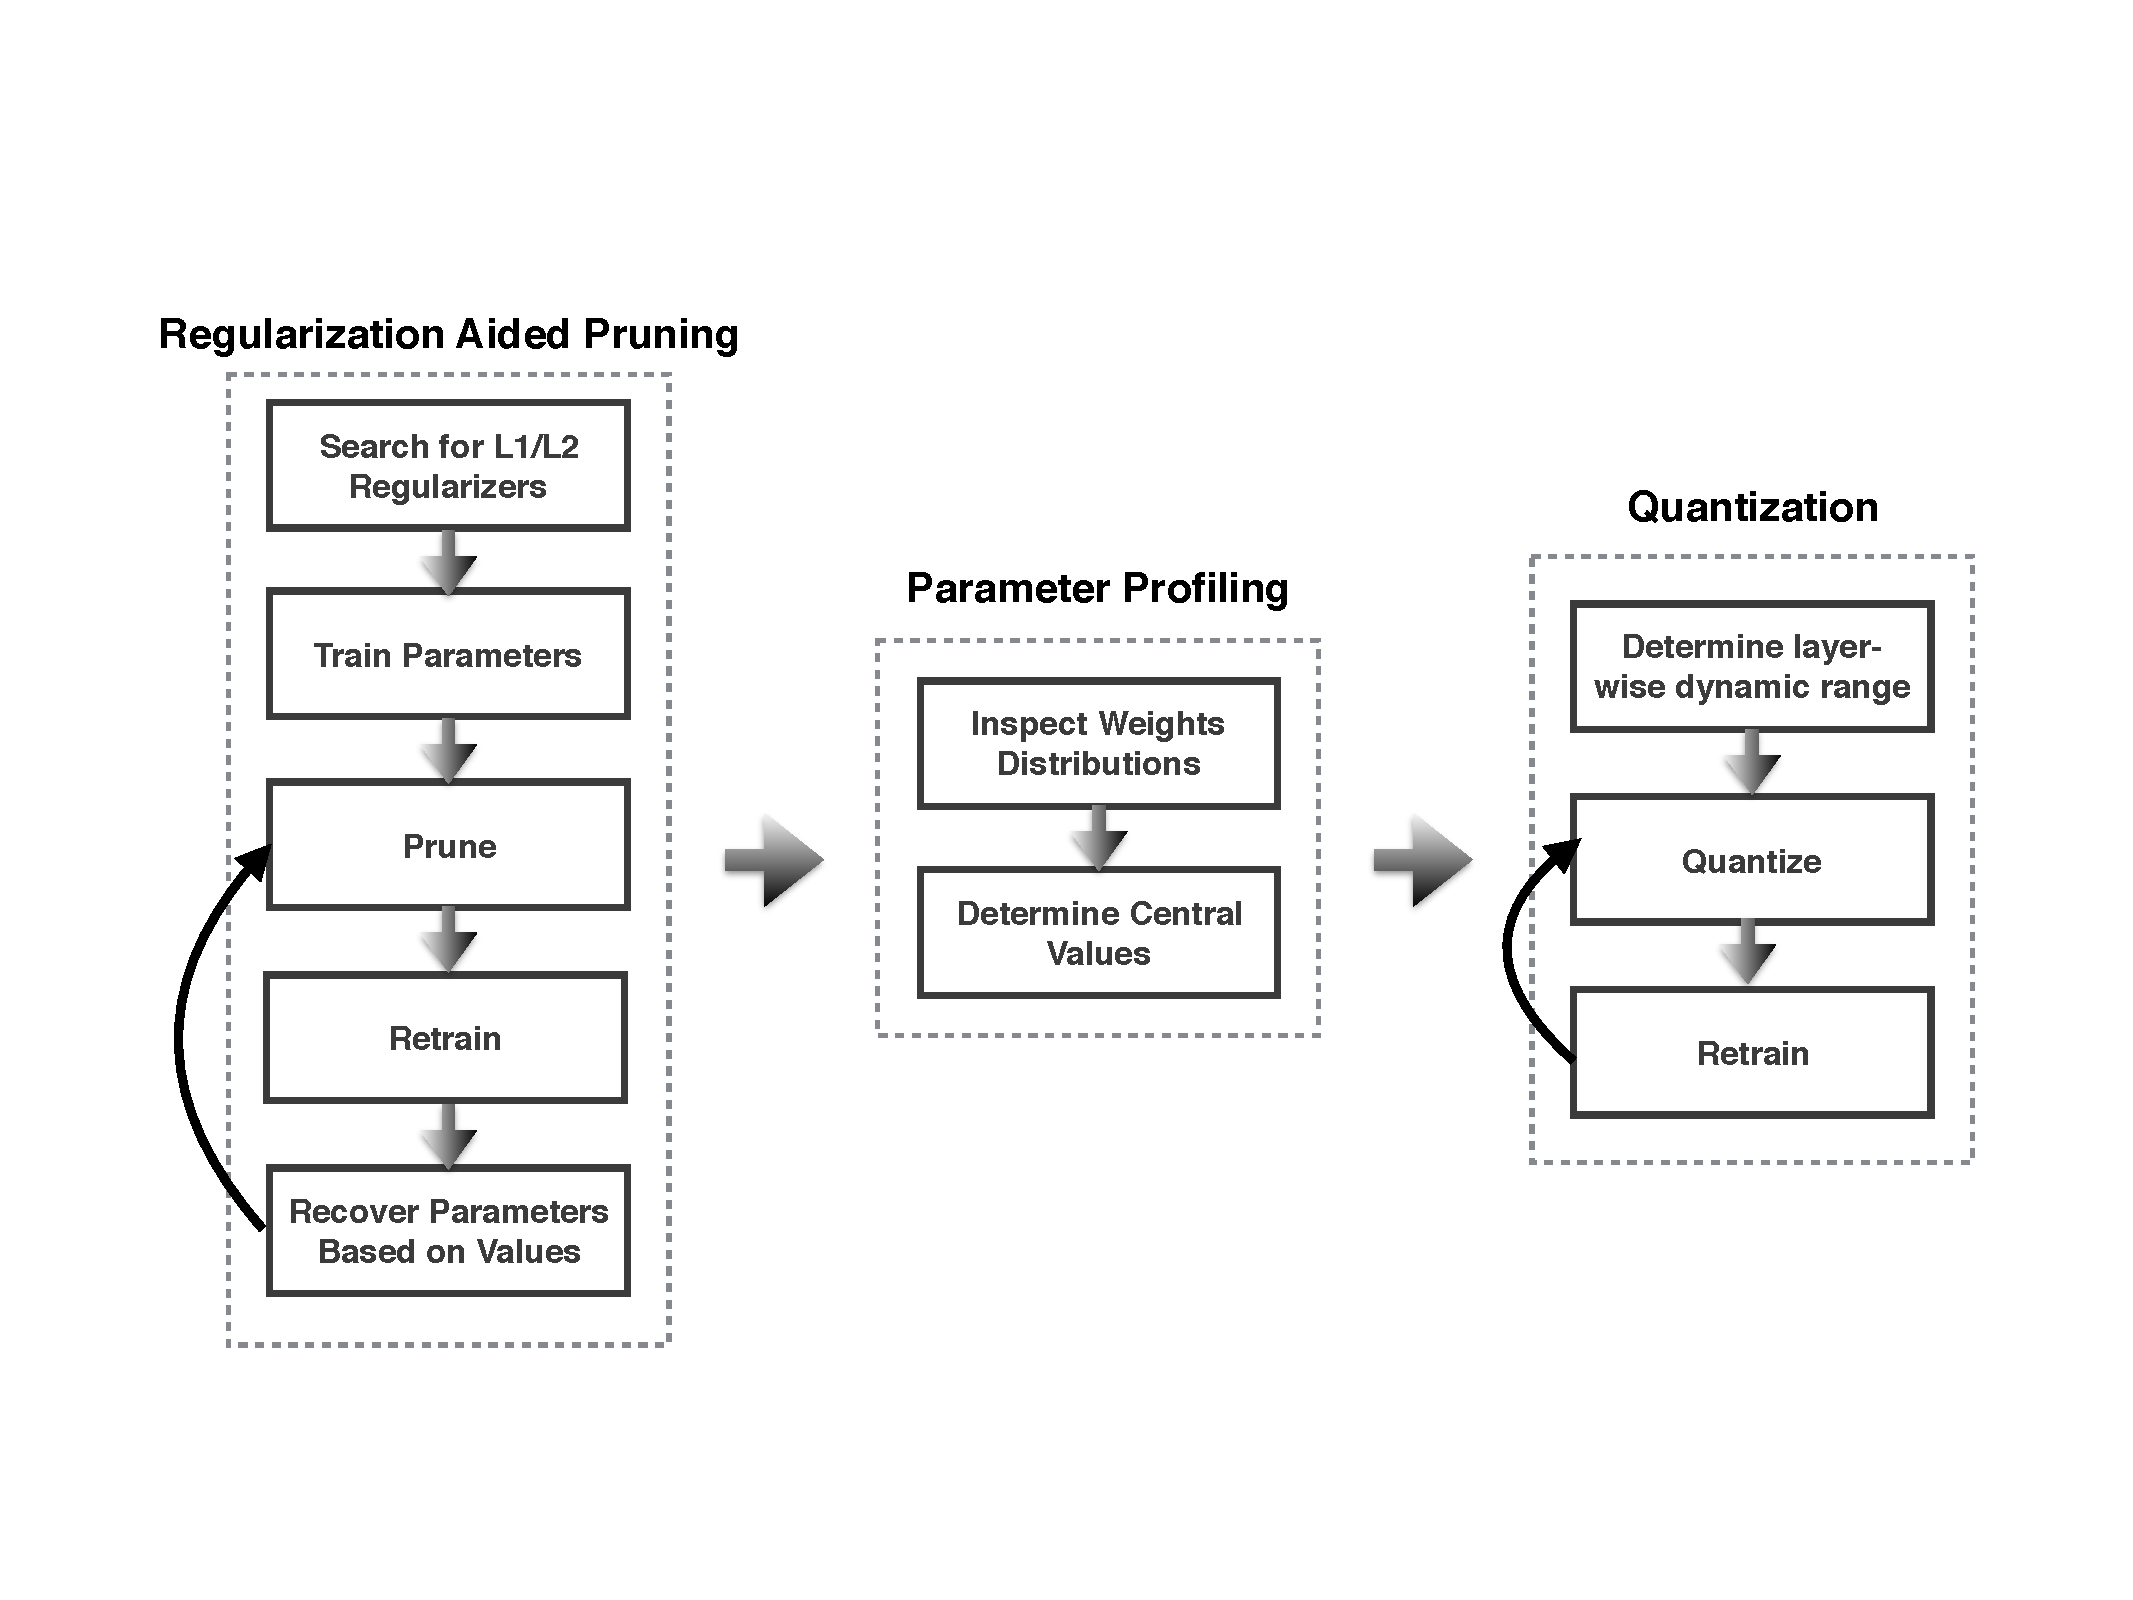
\includegraphics[width=\textwidth]{fig_proposed_flow.pdf}
  \caption{Overview of the proposed compression pipeline.}
  \label{fig:proposed_compression_flow}
\end{figure}

In my implementation, the focus stays on pruning and quantization, an overview
of the complete compression pipeline is shown in \Cref{fig:proposed_compression_flow}.
\textit{Regularization aided pruning} is performed to reduce the number of
parameters in a neural network.
The best hyperparameter combinations for the regularizer come from an exhaustive
search.
The rest of the pruning process is identical to \textit{Dynamic network surgery}, where
pruned weights have a chance to recover.
The second phase is to profile the parameters, this profiling serves quantization
since some important information is extracted from the pre-quantized model and
the central values are determined.
The quantization method used is \textit{Centralized dynamic fixed-point quantization}.
The dynamic ranges are stored in a layer-wise fashion, each quantization is
combined with retraining to recover the test accuracies.

\section{Evaluation of Performance}
To fully understand the performance difference between my proposed compression
pipeline and \textit{Deep Compression}, \Cref{tab:comp_summary} summarizes the
performances of the two compression pipelines on \textit{LeNet5}.

\begin{table}[!h]
  \centering
  \begin{tabular}{lllllll}
    \hline
    Model   &Layer     &Params    &\%(\textit{Han}, P)  &\%(\textit{Han}, P+Q)  &\%P        &\%P+Q 	\\
    \hline
    LeNet5  &cov1     &0.5K       &66\%                 &78.5\%                 &78.9\%     &12.2\%\\
            &cov2     &25K        &12\%                 &6.0\%                  &7.5\%      &1.2\%\\
            &fc1      &400K       &8\%                  &2.7\%                  &0.3\%      &0.047\%\\
            &fc2      &5K         &19\%                 &6.9\%                  &67.1\%     &10.5\%\\
    \hline
            &total (CR)    &431K       &8\%(12x)             &3.05\%(33x)            &1.6\%(63x) &0.25\%(403x)\\
    \hline
            &ER       &-          &$0.8\%$               &$0.8\%$               &$0.64\%$   &$0.64\%$\\
    \hline
  \end{tabular}
  \caption{\textit{LeNet5} compression summary, Pruning and Quantization, CR is the compression
  rate, ER is the error rate. P represnets pruning and Q reporesents quantization.}
  \label{tab:comp_summary}
\end{table}

As shown in \Cref{tab:comp_summary}, putting a \textit{LeNet5} into the proposed
compression pipeline, the neural network obtains a compression rate of $403$x.
This compression rate shows an $12$x increase compared to \textit{Deep Compression}.
In terms of pruning, \textit{Regularization aided pruning} provides a better result,
showing an increase of $5.25$x compared to \textit{Determnisitc pruning}.
The proposed compression pipeline uses \textit{Centralized dynamic fixed-point
arithmetic} and quantized the entire model to 5 bits.

It is also important to note that the use of \textit{Weights sharing} in
\textit{Deep Compression} gives significant energy overhead.
Each weight now is encoded using a codebook.
When neural network inference occurs, each weight fetches the correct value
using the stored index as an address.
This extra weights fetching process is the cost of using \textit{Weights sharing}.
\textit{Yang et al.} suggested one of the major energy consumption in network
inference is data movement \cite{Tien}.
Since \textit{Weights sharing} added this redundant data movement, its energy
consumption should be evaluated more carefully for understanding the trade-off between
energy savings and compression rates.
In contrast, using \textit{Centralized dynamic fixed-point
arithmetic}, the arithmetic operators can be designed specifically for this kind
of arithmetic and thus avoids the weights fetching stage.

\begin{table}[!h]
  \centering
  \begin{tabular}{lllll}
    \hline
    Model   &Layer     &Params     &\%P        &\%P+Q 	\\
    \hline
    CifarNet  &cov1     &4.8K      &55\%     &10.3\%\\
            &cov2     &102.4K    &12\%      &2.3\%\\
            &fc1      &885K      &4\%      &0.75\%\\
            &fc2      &74K       &24\%     &4.5\%\\
            &fc3      &2K        &60\%     &11.2\%\\
    \hline
            &total(CR)    &1068K     &6.5\%(15.4x) &1.2\%(82.2x)\\
    \hline
            &ER       &-         &$18\%$   &$18\%$\\
    \hline
  \end{tabular}
  \caption{\textit{CifarNet} compression summary, Pruning and Quantization, CR is the compression
  rate, ER is the error rate. P represnets pruning and Q reporesents quantization.}
  \label{tab:comp_summary2}
\end{table}
As stated in \Cref{tab:comp_summary2}, pruning offers a compression rate
of $15.4$x. Combinging pruning with quantization, the proposed compression pipeline
offers a compression rate of $82.2$x on \textit{CifarNet} without any loss of
test accuracy.

\section{Evaluation of Compression Techniques}
In my compression pipeline, two main phases are pruning and quantization.
The experimental results of various pruning techniques are summarized in
\Cref{sec:pruning_sum}.
Non-deterministic pruning methods are generally better than deterministic
pruning.
The best performance pruning strategy is \textit{Regularization aided pruning},
however, it might take a significantly larger amount of time depending on how
experienced the designer is in finding the correct regularization parameters.
In contrast, \textit{Dynamic network surgery} also proves to have good compression
rates and avoids the efforts of searching for the regularization hyperparameters.

In terms of quantization, the suitable methods for pruned and unpruned models
are different.
For unpruned models, \textit{Customized floating-point} proves its performance is
comparable to the popular \textit{Dynamic fixed-point} arithmetic, moreover,
it does not restrict any dynamic ranges in the number representation system.
Consider pruned models, an idea of re-centralizing the arithmetic representations
is suggested, and \textit{Centralized dynamic fixed-point} arithmetic achieved the
best performance.




\chapter{Summary and Conclusions}
\section{Conclusion}
In this project, I have investigated a number of pruning and quantization methods
and built a complete compression pipeline based on the methods that have
the best performances.
A number of existing pruning and quantization methods have been explored in this project,
and they are listed below:
\begin{enumerate}
  \item Deterministic pruning
  \item Dynamic network surgery
  \item Fixed-point quantization
  \item Dynamic fixed-point quantization
\end{enumerate}
Inspired by these existing compression techniques,
some novel pruning and quantization methods are also proposed:
\begin{enumerate}
  \item Gradient profiling pruning
  \item Regularization aided pruning
  \item Customized floating-point quantization
  \item Re-centralized quantization
\end{enumerate}

The large range of exploration of compression techniques provided some important
empirical results.
For pruning, as summarized previously in \Cref{sec:pruning_ext_comp} and \Cref{sec:pruning_sum},
it can be concluded that pruning only weights and pruning in a non-deterministic
manner give significantly better compression results.
Regularizations also help improving the compression rates.
The proposed pruning strategy, \textit{Regularization aided pruning}, becomes
the best performance pruning method.
In terms of quantization, the results suggest \textit{Customized floating-point
quantization} achieves best quantization results on unpruned models due to its
ability of tracking near-zero numbers to high precisions.
Later, for pruned neural networks, re-centralization of arithmetics gives significant improvement on
pruned model.
The practical results proved that the preferred arithmetics are different for dense and
sparse network models because of the difference in weights distributions.

At the end, I selected \textit{Regularization aided pruning} and \textit{Centralized dynamic fixed-point
quantization}
for building a complete compression pipeline.
The proposed compression pipeline achieves a better compression results than the
existing compression pipeline (\textit{Deep Compression}).
On the \textit{LeNet5} model, the proposed compression pipeline ($403$x) shows a significant
advance in compression rate compared to \textit{Deep Compression} ($33$x).
On the \textit{CifarNet} model, the proposed compression pipeline achieved a
compression rate of $82.2$x.

\section{Future Works}
Possible future works can be broken down into two parts: pruning and quantization.
One possible future work is to focus on reducing the retraining time in pruning.
Most pruning methods require at least one complete retraining after the pruning
process \cite{Thimm, Li2016}.
Shorten the retraining time can significantly reduce the computation time,
but it might cause a bad compression result.
\textit{Gradient profiling pruning} shows promising results with limited retraining
resources.
It obtains information of the importance of weights during retraining and uses this
information to prune weights in a more selective manner.
However, its performance should be further verified on other networks.
\textit{Regularization aided pruning} is proven useful in achieving high
compression rates.
The amount of time spent on choosing feasible hyperparameters for regularizers
are entirely empirical at this stage.
One possible future work is to automate this process.
It has been empirically observed that the feasible regularization loss (loss caused by regularizers)
is around ten percents of the value of the cost function.
If such a numerical ratio can be confirmed on a large range of networks, it is
easy to automate the hyperparameter definitions by inspecting this numerical ratio
at run-time.
Another potential future work is to explore more efficient regularizers.
Regularizers help pruning because they encourage sparsity during the retraining
phase.
It is therefore logical to consider using regularizers that are better at
encouraging zeros for achieving a better compression.
\textit{Shakeout} is a new regularizer proposed by \textit{Kang et al.} \cite{Kang}.
\textit{Kang et al.} proved \textit{Shakeout} encourages more sparsity than
traditional $l_1$ and $l_2$ norms \cite{Kang}.
It is possible to use \textit{Shakeout} as a regularizer for \textit{Regularization adided pruning}
in future developments.

With respect to quantization, I have demonstrated that \textit{Customized floating-point}
can be more efficient than the popular \textit{Dynamic fixed-point} method when
the neural network model is dense.
It is noted that \textit{Dynamic fixed-point} arithmetic fails to recover
test accuracies if the trained network is sensitive to reduced dynamic ranges.
A theoretical proof and more throughout experimentations should carry on
in this direction to prove whether this is a general phenomenon.
Some novel arithmetics, such as logarithmic arithmetics, are catching attentions
recently \cite{tann2017hardware} because they can compute multiplications
in a power-efficient manner.
Part of the future works is to propose energy consumption models for the
proposed arithmetic operators in this project.
These energy estimations could be helpful for exploring possible hardware
accelerator architectures.

In this project, pruning and quantization are treated as individual stages and
retraining takes place in each of these stages.
One interesting future work is to combine pruning, quantization and
retraining all in one stage.
Previously, a number of research works have tried to combine pruning with
retraining into one process and thus eliminates the need of pruning iteratively
\cite{Hassibi, DBLP:journals/corr/MolchanovTKAK16}.
The strategy is to add the number of zeros of weights masks into the cost function so that the
network encourages more values to be pruned away.
It is interesting to see whether there is a chance to fit quantization into this
method, for instance, the bit-width might be considered as a metric in the cost
function and a lower bit-width is preferred.

Another important future work is to apply the proposed compression pipeline to
a larger number of neural networks.
Networks, like \textit{AlexNet} \cite{Krizhevsky}, \textit{VGGNet} \cite{DBLP:journals/corr/SimonyanZ14a}
and \textit{InceptionNet} \cite{szegedy2015going}, should be tested on the
proposed compression pipeline.
\appendix
\singlespacing

\bibliographystyle{unsrt}
\bibliography{dissertation}

\end{document}
